\documentclass[openright,final,fmstyle]{utnfrrotesis}
\usepackage[utf8]{inputenc}
\usepackage[spanish]{babel}
\usepackage[authoryear,datebegin,nonamereplace,sort&compress]{flexbib}
\usepackage{titlesec}
\usepackage{amsmath}
\usepackage{paralist} % it provides the inparaenum environment
\usepackage{pgfgantt}
\usepackage{enumerate}
\usepackage[inline]{enumitem}
\usepackage{fancyvrb}
%\usepackage{import}
\graphicspath{{imagenes/}} % Necesario para importar las figuras en PDF.
% (with an optional formatting specification in square brackets): To change the styles of the counter,
% tokens A, a, I, i, and 1 can be used in the optional argument to produce the counter with one of the styles
% \Alph, \alph, \Roman, \roman and \arabic. For example:
%
% \begin{inparaenum}[(i)]
%
% produces the labels (i), (ii), (iii) ...

%%%%%%%%%%%%%%%%%%%%%%%%%%%%%%%%%%%%%%%%%%%%%%%%%%%%%%%%%%%%%%%%%%%%%%%%%%%%%%%%%%%%%%%%%%%%%%%%%%%%%%%%
%%% paquete para comillas
%%%%%%%%%%%%%%%%%%%%%%%%%%%%%%%%%%%%%%%%%%%%%%%%%%%%%%%%%%%%%%%%%%%%%%%%%%%%%%%%%%%%%%%%%%%%%%%%%%%%%%%%
\usepackage{quotmark}

%%%%%%%%%%%%%%%%%%%%%%%%%%%%%%%%%%%%%%%%%%%%%%%%%%%%%%%%%%%%%%%%%%%%%%%%%%%%%%%%%%%%%%%%%%%%%%%%%%%%%%%%
%%% para guionado
%%%%%%%%%%%%%%%%%%%%%%%%%%%%%%%%%%%%%%%%%%%%%%%%%%%%%%%%%%%%%%%%%%%%%%%%%%%%%%%%%%%%%%%%%%%%%%%%%%%%%%%%
\usepackage{hyphenat}
\usepackage{booktabs}
\usepackage{bm}
%\usepackage{bera} % optional: just to have a nice mono-spaced font
\usepackage{listings}
\usepackage{xcolor}
\usepackage{colortbl}
\usepackage{multicol}
\usepackage{supertabular}
\usepackage{multirow}
\usepackage[english,vlined,linesnumbered]{algorithm2e}
\usepackage{pdflscape}
\usepackage{fullpage,graphicx}
\usepackage{rotating}
\usepackage[hidelinks]{hyperref}
\usepackage{graphicx}
\usepackage{verbatim}
\usepackage{pgfplots}
\usepackage{pgfplotstable}
\usepackage{filecontents}
\usepackage{tabularx,ragged2e,booktabs,caption}

\newcolumntype{L}{>{\RaggedRight\arraybackslash}X}

\hypersetup{
	pdftitle={Tesis de Maestría en Ingeniería en Sistemas de Información},
	pdfauthor={Ing. Federico Tesone},
	pdfsubject={Desarrollo de una medida de similaridad para Sistemas de Recomendación en sitios de Community Question Answering. Análisis desde un enfoque Big Data y usando un método de ensamble de clustering},
	pdfkeywords={},
	bookmarksnumbered=true,
	bookmarksopen=true,
	bookmarksopenlevel=1,
	colorlinks=false,
	pdfstartview=Fit,
	allcolors=blue
}

\usepackage{nowidow}
\widowpenalty=5000
\clubpenalty=10000

\SetKwIF{If}{ElseIf}{Else}{si}{entonces}{sin\'o, si}{de lo contrario}{fin si}
\SetKwInput{KwIn}{Entrada}%
\SetKwInput{KwOut}{Salida}%
\SetKwInput{KwData}{Datos}%
\SetKwInput{KwResult}{Resultado}%
\SetKw{KwTo}{a}%
\SetKw{KwRet}{devolver}%
\SetKw{Return}{devolver}%
\SetKwBlock{Begin}{inicio}{fin}%
\SetKwRepeat{Repeat}{repetir}{hasta que}%
\SetKwFor{ForEach}{para cada}{hacer}{fin para cada}
\SetKwFor{While}{mientras}{hacer}{fin mientras}
\SetKwFor{For}{para}{hacer}{fin para}%

\setcounter{secnumdepth}{4}
\setcounter{tocdepth}{4}

%%%%%%%%%%%%%%%%%%%%%%%%%%%%%%%%%%%%%%%%%%%%%%%%%%%%%%%%%%%%%%%%%%%%%%%%%%%%%%%%%%%%%%%%%%%%%%%%%%%%%%%%
% para remediar el problema de babel de abreviaciones de teclado para la virgulilla
%%%%%%%%%%%%%%%%%%%%%%%%%%%%%%%%%%%%%%%%%%%%%%%%%%%%%%%%%%%%%%%%%%%%%%%%%%%%%%%%%%%%%%%%%%%%%%%%%%%%%%%%
\addto\shorthandsspanish{\spanishdeactivate{~}}

%para los nombres a lo largo del documento
\newcommand{\gss}{$\gamma$-AM}
\newcommand{\disc}{percentil}
\newcommand{\Disc}{Percentil}
\newcommand{\Sim}{\text{Sim}}
\newcommand{\tfill}{1mm}
\newcommand{\tffill}{-10mm}
\newcommand{\tftfill}{-6mm}
\newcommand{\fffill}{-6mm}
\newcommand{\bfill}{-10mm}
\newcommand{\clusteryea}{8}
\newcommand{\clusterara}{9}
\newcommand{\geneexampleyea}{POP2}
\newcommand{\geneexampleara}{AT2G19450}
\newcommand{\classico}{Rhee \emph{et al.} approach \cite{rhee2008use}}
\newcommand{\classic}{Rhee \emph{et al.} approach}
\newcommand{\classi}{Rhee \emph{et al.} \cite{rhee2008use}}
\newcommand{\arafull}{\emph{Arabidopsis thaliana}}
\newcommand{\ara}{\emph{A. thaliana}}
\newcommand{\yeafull}{\emph{Saccharomyces cerevisiae}}
\newcommand{\yea}{\emph{S. cerevisiae}}
\newcommand{\km}{$k$-medias}

\newcommand{\given}{\Big\vert}

\usepackage[a4paper,footskip=.5in]{geometry}

%subsubsub
\titleformat{\paragraph}
{\normalfont\normalsize\bfseries}{\theparagraph}{1em}{}
\titlespacing*{\paragraph}{0pt}{3.25ex plus 1ex minus .2ex}{1.5ex plus .2ex}

%para quitar de a una línea en algorithm2e
\makeatletter
\newcommand{\nosemic}{\renewcommand{\@endalgocfline}{\relax}}% Drop semi-colon ;
\newcommand{\dosemic}{\renewcommand{\@endalgocfline}{\algocf@endline}}% Reinstate semi-colon ;
\newcommand{\pushline}{\Indp}% Indent
\newcommand{\popline}{\Indm\dosemic}% Undent
\let\oldnl\nl% Store \nl in \oldnl
\newcommand{\nonl}{\renewcommand{\nl}{\let\nl\oldnl}}% Remove line number for one line
\makeatother

\title{Desarrollo de una medida de similaridad para Sistemas de Recomendación en sitios de Community Question Answering. Análisis desde un enfoque Big Data y usando un método de ensamble de clustering}
\author{Ing. Federico Tesone \vspace{-6mm} }
\degree{Maestría en Ingeniería en Sistemas de Información}
\advisor{Dr.} {Guillermo Leale}
\coadvisor{Dra.} {Soledad Ayala}
\institution{Universidad Tecnológica Nacional}
\faculty{Facultad Regional Rosario}

\renewcommand\thesection{\arabic{section}}
\interfootnotelinepenalty=10000 %  Para que las footnote no se pasen a la otra pagina.

% To write JSON files
\colorlet{punct}{red!60!black}
\definecolor{background}{HTML}{FFFFFF}
\definecolor{delim}{RGB}{20,105,176}
\colorlet{numb}{magenta!60!black}

%%%%% LANGUAGES AND SNIPPETS
\renewcommand{\lstlistingname}{Fragmento de código} % Redefinicion de la palabra "Listing" para caption de snippet the codigo.

% JSON
\lstdefinelanguage{json}{
	basicstyle=\footnotesize\ttfamily,
	showstringspaces=false,
	breaklines=true,
	tabsize=2,
	backgroundcolor=\color{background},
	literate=
	*{0}{{{\color{numb}0}}}{1}
	{1}{{{\color{numb}1}}}{1}
	{2}{{{\color{numb}2}}}{1}
	{3}{{{\color{numb}3}}}{1}
	{4}{{{\color{numb}4}}}{1}
	{5}{{{\color{numb}5}}}{1}
	{6}{{{\color{numb}6}}}{1}
	{7}{{{\color{numb}7}}}{1}
	{8}{{{\color{numb}8}}}{1}
	{9}{{{\color{numb}9}}}{1}
	{:}{{{\color{punct}{:}}}}{1}
	{,}{{{\color{punct}{,}}}}{1}
	{\{}{{{\color{delim}{\{}}}}{1}
	{\}}{{{\color{delim}{\}}}}}{1}
	{[}{{{\color{delim}{[}}}}{1}
	{]}{{{\color{delim}{]}}}}{1},
}

% PYTHON

% Default fixed font does not support bold face
\DeclareFixedFont{\ttb}{T1}{txtt}{bx}{n}{12} % for bold
\DeclareFixedFont{\ttm}{T1}{txtt}{m}{n}{12}  % for normal

% Custom colors
\usepackage{color}
\definecolor{deepblue}{rgb}{0,0,0.5}
\definecolor{deepred}{rgb}{0.6,0,0}
\definecolor{deepgreen}{rgb}{0,0.5,0}

% Python style for highlighting
\newcommand\pythonstyle{\lstset{
		language=Python,
		morekeywords={self},              % Add keywords here
		keywordstyle=\footnotesize\color{deepblue},
		emph={MyClass,__init__},          % Custom highlighting
		emphstyle=\footnotesize\color{deepred},    % Custom highlighting style
		stringstyle=\color{deepgreen},
		frame=tb,                         % Any extra options here
		showstringspaces=false,
  		basicstyle=\footnotesize,
		numbers=left,
		stepnumber=1
}}


% Python environment
\lstnewenvironment{python}[1][]
{
	\pythonstyle
	\lstset{#1}
}
{}

% Python for external files
\newcommand\pythonexternal[2][]{{
		\pythonstyle
		\lstinputlisting[#1]{#2}}}

% Python for inline
\newcommand\pythoninline[1]{{\pythonstyle\lstinline!#1!}}

%%%%%%% R Language
\lstset{commentstyle=\color{red},keywordstyle=\scriptsize\color{black},showstringspaces=false}
\lstnewenvironment{rc}[1][]{\lstset{keywordstyle=\scriptsize,language=R}}{}
\newcommand{\ri}[1]{\lstinline{#1}}  %% Short for 'R inline'

\lstset{keywordstyle=\scriptsize,language=R}             % Set R to default language

\usepackage{etoolbox}
\makeatletter
\patchcmd{\@verbatim}
{\verbatim@font}
{\verbatim@font\small}
{}{}
\makeatother

\renewcommand\tabularxcolumn[1]{m{#1}}% for vertical centering text in X column

\begin{document}
	\maketitle

	\newgeometry{left=4.06cm,top=2.54cm,right=2.54cm,bottom=2.54cm}

	\hfill \textit{A mi persona favorita.}

	\abstract

Los \textit{Sistemas de Recomendación} (Recommender Systems o RS) tienen la tarea de recomendar ítems a los usuarios de un sitio o aplicación. Los mismos pueden ser aplicados a sitios de preguntas y respuestas colaborativas, llamados \textit{Community Question Answering} (CQA por sus siglas en inglés) y las preguntas que realizan los usuarios de la aplicación pueden considerarse como los ítems a recomendar. En este trabajo, son de interés las preguntas pendientes de ser respondidas, ya que la tarea de recomendar otras preguntas similares que hayan sido formuladas por otros usuarios y tengan la respuesta deseada, puede ser realizada por un RS, minimizando así el tiempo en que un usuario puede encontrar lo que estaba buscando.

\bigskip Un buen RS debería utilizar una medida de \textit{similaridad} confiable entre preguntas, por lo cual proponemos crear una nueva medida combinada de distancia para textos a través de un método de ensamble de clustering basado en acumulación de evidencias, utilizando una arquitectura Big Data. Para este fin, dispondremos de un conjunto de datos de pares de preguntas reales, extraídos del sitio web Quora. Se realizará un análisis comparativo entre el método de ensamble de clustering y las medidas de similaridad utilizadas como punto de partida del mismo.

\bigskip Este tipo de enfoque es necesario para trabajar con grandes conjuntos de datos y así recuperar, analizar y procesar los mismos con precisión, variabilidad y velocidad, con el propósito de encontrar una medida de similaridad que pueda presentarse como una alternativa a las actuales en términos de mejorar la experiencia del usuario en sitios de CQA, mejorar las medidas de rendimiento y reducir las probabilidades de error en la búsqueda de preguntas similares.

\bigskip

\noindent\textbf{Palabras clave:} Community Question Answering, Recommender Systems, Big Data, Clustering, Clustering Ensemble, Evidence Accumulation, Text Similarity.

	\tableofcontents % Tabla de contenidos
	\sloppy % Indica a LaTex que debe minimizar el corte de las palabras para pasar de una línea a otra.
	% \mainmatter % para reiniciar numeración.

	\listoftables
	\listoffigures
    \acknowledgements

	\pagestyle{plain} % Paginas sin encabezado, pero con numero de pagina.

	\chapter*{Capítulo 1. \textbf{Introducción}}\label{ch:introduccion}
\addcontentsline{toc}{chapter}{Capitulo 1. Introducción}

\section*{}
\addtocounter{section}{1}
\setcounter{subsection}{0}

\subsection{Área temática}
Los sitios de \textit{Community Question Answering} (CQA) brindan servicios que permiten a los usuarios formular y contestar preguntas sobre temas de cualquier índole. Miles de nuevas preguntas son subidas diariamente en sitios de CQA como Yahoo! Answers\footnote{Yahoo! Answers: \url{https://answers.yahoo.com/}. Último acceso: Julio 2021.}, Stackexchange\footnote{Stackexchange: \url{https://stackexchange.com/}. Último acceso: Julio 2021.}, Stackoverflow\footnote{Stackoverflow: \url{https://stackoverflow.com/}. Último acceso: Julio 2021.}, o Quora\footnote{Quora: \url{https://www.quora.com/}. Último acceso: Julio 2021.}. Estos son portales muy populares donde los usuarios suben diariamente una cantidad importante de preguntas de varios dominios para obtener respuestas de otros usuarios de la comunidad \citep{anuyah2017can}. Del análisis de sitios de CQA, puede observarse que muchas de las preguntas no están respondidas correctamente o no tienen respuestas específicas, ya que, en estas comunidades, hay típicamente un pequeño número de expertos entre la gran población de usuarios \citep{yang2013cqarank}. Por lo tanto, cuando un usuario realiza una pregunta, es de interés buscar si esa misma interrogación ha sido formulada por otro usuario con anterioridad y para verificar que tenga la respuesta buscada. Con esto, el usuario podría leer las respuestas a dicha pregunta sin tener que esperar que la misma sea respondida. Esto no siempre es una tarea fácil, ya que podría darse la situación en la que la pregunta sí exista previamente en el sitio y haya sido respondida y, sin embargo, esté formulada de una manera completamente diferente en el sentido léxico. Por esta razón, una correspondencia exacta (o casi exacta) no es aplicable. Consideremos el siguiente ejemplo, a partir del análisis de dos preguntas cuya respuesta final es la misma: \textit{¿Cómo elijo una revista para publicar mi artículo?} y \textit{¿Dónde publico mi artículo?}\footnote{Traducción de las preguntas “How do I choose a journal to publish my paper?, Where do I publish my paper?” extraídas desde el conjunto de datos de Quora que se utilizará en el presente trabajo de tesis \url{https://quoradata.quora.com/First-Quora-Dataset-Release-Question-Pairs}. Último acceso: Julio 2021.}. Entre estas dos interrogaciones, existe apenas una superposición de palabras, sin tener en cuenta los \textit{stopwords}\footnote{En informática, se llama stopword a palabras que se filtran antes o después del procesamiento de datos del lenguaje natural \citep{leskovec2014mining}.}. Sin embargo, ambas preguntas tienen la misma respuesta, que referirá a revistas o sitios donde publicar un artículo científico.

\bigskip Con el fin de comparar dos preguntas, se establece entonces una medida de similaridad que se puede considerar como máxima cuando son idénticas y que es inversamente proporcional a las diferencias entre ellas \citep{lin1998information}. Pero teniendo en cuenta que una medida de similaridad de texto entre preguntas basada en características léxicas no las detectaría como preguntas iguales. Esto deja en evidencia la necesidad de utilizar enfoques que, además, consideren características semánticas.

\bigskip A partir de lo expuesto anteriormente, puede decirse que la tarea de encontrar preguntas similares en sitios de CQA puede ser llevada a cabo por un Sistema de Recomendación. Los Sistemas de Recomendación (Recommender Systems o RS) son herramientas de software y técnicas que proveen sugerencias de ítems, bajo el supuesto de que es posible que los usuarios tengan la intención de utilizar dichos ítems \citep{ricci2011introduction}. Las sugerencias relacionan una variedad de procesos de toma de decisiones, como por ejemplo qué artículos comprar o qué música escuchar. El término general usado para denotar lo que los RS recomiendan a los usuarios es el vocablo “\textit{Ítem}”. Los ítems son objetos que pueden estar caracterizados por su valor o utilidad. El valor de un ítem puede ser positivo si el ítem es útil para el usuario y negativo si no es apropiado. En este último caso, el usuario tomaría una mala decisión al seleccionarlo. A partir de la dinámica que se construye en los RS, las recomendaciones al usuario pueden ser personalizadas o no personalizadas. Las primeras, se basan en los comportamientos del usuario o en grupos de usuarios para encontrar sugerencias adecuadas a sus preferencias; las segundas, efectúan recomendaciones que son inherentes a los ítems que el RS sugerirá. Cada una de estas estrategias de recomendación se elabora a partir de los diferentes conocimientos y datos recopilados por el sitio o el sistema donde el RS esté aplicado. Algunos ejemplos de tales aplicaciones incluyen la recomendación de libros, películas, o ítems de compra de productos y/o servicios \citep{adomavicius2005toward}. En particular, para los sitios de CQA, los algoritmos de recomendación se aplican principalmente a elementos de texto. Este trabajo se centrará en ese tipo de recomendaciones, que pueden estar clasificadas dentro de RS basados en contenido de texto no personalizados, ya que las mismas están basadas únicamente en la estructura sintáctica y semántica de las preguntas existentes en los sitios de CQA. Los usuarios pueden navegar esas recomendaciones. Luego, pueden aceptarlas o no y, además, proveer inmediatamente o en un paso posterior, una retroalimentación explícita o implícita.

\bigskip A consecuencia de lo expuesto anteriormente, y sumado a que se dispone de un gran conjunto de datos, se diseñó e implementó una propuesta de arquitectura para utilizar Big Data con el fin de crear una medida de similaridad de texto que alimente a un RS especializado en la tarea de encontrar preguntas similares en sitios de CQA basado en análisis de contenido de texto. Este tipo de enfoque es necesario para procesar una gran cantidad de datos y, de esta manera, optimizar el procesamiento de los mismos, logrando velocidad y con la ventaja de poder aprovechar toda la variabilidad que provee un conjunto de datos de gran volumen. Luego de obtener esta nueva medida de similaridad, se realizará un análisis comparativo de la misma contra las medidas subyacentes utilizadas como entrada del método en cuestión, utilizando la arquitectura en Big Data propuesta.

\subsection{Tema específico}
Con el fin de dejar en claro el alcance de este trabajo, se toma como punto de partida el trabajo de investigación de la Universidad Tecnológica Nacional, Facultad Regional Rosario: “Comparative Analysis on Text Distance Measures Applied to Community Question Answering Data” \citep{gonzalez2017comparative}, el cual se centra en el Paso 1 de la secuencia de pasos (o \textit{pipeline}) que se describe en la Figura \ref{fig:pipeline}.
\bigskip
\begin{figure}[h!]
	\centering
	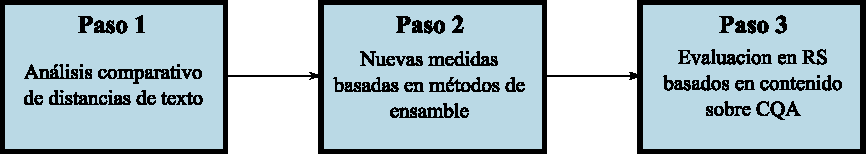
\includegraphics[width=0.9\linewidth]{5_introduccion/imagenes/pipeline}
	\caption{Pipeline para un RS basado en contenido de CQA y en una nueva medida de similaridad.}
	\label{fig:pipeline}
\end{figure}

Este proceso descrito en tres pasos, tiene como objetivo construir un RS basado en una medida novedosa de similaridad de texto. En el Paso 1 se realiza un análisis comparativo desarrollado a partir de medidas basadas en distancia; en el Paso 2, se crea una nueva medida construyendo una matriz de similaridad basada en ensamble de clustering, como una de las propuestas en los métodos \textit{Algoritmo de Particionamiento de Similitud basado en Cluster} (Cluster-based Similarity Partitioning Algorithm o CSPA) \citep{strehl33knowledge} y \textit{Clustering de Acumulación de Evidencias} (Evidence Accumulation Clustering o EAC) \citep{fred2005combining}. El método EAC, que será descrito en detalle más adelante, intenta mejorar la calidad de salida para una representación de similaridad basada en texto; por último, en el Paso 3 se debe aplicar la matriz de similaridad obtenida en el Paso 2 en un RS basado en contenido, con el fin de evaluar su eficacia en sitios de CQA.

\bigskip Si tomáramos el conjunto completo de datos Quora (404301 pares de preguntas, es decir, 808602 preguntas totales), y quisiéramos generar una sola matriz de distancias cruzando par a par todas las preguntas entre sí, estaríamos calculando $\frac{n(n+1)}{2} = 326919001503$ distancias, donde $n = 808602$ y el resultado es la cantidad de elementos en la triangular superior de la matriz cuadrada donde las preguntas corresponden a la vez a las filas y a las columnas. El ejemplo anterior sirve para tomar dimensión del volumen de datos que es necesario manejar con este enfoque basado en ensamble de clustering. Esta matriz considera sólo una de las técnicas de distancia de texto del estado del arte, por lo cual si deseamos combinar varias técnicas mediante un método de ensamble, deberíamos generar al menos una matriz por cada una de ellas, y luego usar las mismas para aplicar EAC. Por lo anterior, estaríamos generando un número total de cálculos considerablemente mayor al que puede procesar una computadora clásica, en un tiempo aceptable. Es necesario además tener en cuenta que las distancias pueden llegar a considerar características diversas entre sí, como morfología, sintaxis y semántica de los textos, lo cual añade complejidad y variedad al volumen considerado. Esta situación plantea la necesidad de considerar una arquitectura Big Data, conjuntamente con optimización de código y técnicas de ejecución paralela entre un gran número de tareas de procesamiento. Con respecto al espacio de almacenamiento, debe notarse que las matrices requieren doble precisión para la representación interna de cada uno de sus elementos (distancias), es decir 750 KB cuando están almacenados en un archivo, por lo cual, si consideramos la matriz ejemplificada anteriormente, necesitaríamos aproximadamente 12 TB para almacenarla, y sería es necesario un esquema de almacenamiento optimizado para la implementación de este método. Con respecto a la velocidad de procesamiento, pruebas preliminares en las técnicas del estado del arte, realizadas con un procesador potente, brindan una estimación de alrededor de 3 años para completar el procesamiento. Con el problema planteado de esta forma, es indispensable aplicar un enfoque de Big Data para satisfacer los requerimientos de volumen, variedad y velocidad que requiere el contexto de análisis, de tal forma de brindar resultados veraces, y de esa forma cumplir con las premisas de las “V” del Big Data\footnote{Las “V” del Big Data refieren a Volumen, Variedad y Velocidad. También se consideran los conceptos de Valor y Veracidad con respecto al resultado de la aplicación del enfoque Big Data \citep{gandomi2015beyond}.}.

\bigskip Este trabajo de tesis apunta entonces a construir una medida de similaridad novedosa desde un enfoque Big Data, tal como se describe en el Paso 2 del pipeline, para luego compararla con las técnicas existentes. Para tal fin, se crea un nuevo software basado en una arquitectura y patrones de Big Data, tomando como punto de partida el desarrollo del estado del arte a partir del trabajo mencionado.

\subsection{Objetivo general}
El presente trabajo de investigación tiene como objetivo construir una arquitectura Big Data que incluye la posibilidad de ser aplicada a grandes conjuntos de datos en el ámbito de CQA y, a partir de esta arquitectura, implementar y evaluar nuevas medidas de similaridad entre textos que puedan ser utilizadas en sistemas de recomendación.

\subsection{Objetivos específicos}
Se detallan a continuación, los objetivos específicos que son necesarios para lograr el objetivo principal.
\begin{itemize}
	\item Diseñar y desarrollar una arquitectura Big Data para cálculo de similaridad en grandes matrices, que requerirá nuevas estrategias para recolectar, procesar y manejar grandes volúmenes de datos.
	\item Identificar medidas de similaridad de texto existentes y un método efectivo de aplicación de las mismas en grandes volúmenes de datos.
	\item Proponer una nueva medida que permita integrar las medidas de similaridad del estado del arte mediante una arquitectura de software basada en Big Data y que sea extensible a otras medidas existentes en el estado del arte.
	\item Evaluar el comportamiento de una medida de similaridad de texto del estado del arte respecto al manejo del volumen, variedad, velocidad y veracidad inherentes a grandes volúmenes de datos, en particular en el ámbito de CQA.
	\item Brindar conclusiones, pautas y recomendaciones para trabajar con medidas de comparación de textos en grandes volúmenes de datos utilizando arquitecturas basadas en Big Data y su aplicación en sistemas de recomendación.
\end{itemize}
	\chapter*{Capítulo 2. \textbf{Fundamentación}}\label{ch:fundamentacion}
\addcontentsline{toc}{chapter}{Capitulo 2. Fundamentación}

\section*{}
\addtocounter{section}{1}
\setcounter{subsection}{0}

\subsection{Motivación de la tesis}
 La calidad de un RS tiene una relación directa con los datos de entrada que se han generado para alimentarlo. Con el fin de generar una entrada basada en medidas de similaridad, es necesaria la comparación de preguntas formuladas en sitios de CQA usando técnicas de análisis de texto. Un problema importante inherente al análisis de texto, con el fin de cuantificar relaciones entre distintos fragmentos o documentos, es encontrar la medida apropiada de representación \citep{gonzalez2017comparative}. Algunas medidas de similaridad resultantes de algoritmos de recomendación en análisis de texto son obtenidas mediante algoritmos puramente sintácticos, léxicos, tales como: Term Frequency \citep{salton5mcgill}, Term Frequency/Inverse Document Frequency \citep{baeza1999modern}, basados en ventanas como FastText \citep{joulin2016fasttext} o Word2Vec \citep{mikolov2013efficient}, o semánticos, como Semantic Distance \citep{li2006sentence}. Los algoritmos puramente sintácticos como Term Frequency y Term Frequency/Inverse Document Frequency tienen conocidos problemas, tales como ser invariantes respecto al orden de las palabras o ser sensibles a stopwords, por lo cual, necesitan un gran trabajo de pre-procesamiento. Adicionalmente, no tienen en cuenta la semántica de las palabras y sus relaciones. FastText y Word2Vec están fuertemente afectados en el orden en el cual aparecen las palabras. Semantic Distance, por su lado, según el trabajo tomado como estado del arte, tampoco alcanza medidas de rendimiento apropiadas para un RS en un sitio de CQA, por ejemplo posee un pobre desempeño en términos de eficiencia debido a su complejidad inherente.

\bigskip Los resultados experimentales de medidas de rendimiento obtenidas en el trabajo que se toma como punto de partida de esta tesis, arrojan entre un \(66.85\%\) y un \(67.97\%\) de exactitud (entre un \(32.03\%\) y un \(33.15\%\) de error) usando cada uno de los algoritmos de recomendación descritos anteriormente. Estos valores son considerados prometedores, ya que las medidas de rendimiento son consistentes en todos los algoritmos seleccionados, lo que denota que la complejidad inherente del conjunto de datos no afecta significativamente el rendimiento de cada uno de ellos. Además, los resultados de prueba no varían significativamente con respecto a los resultados de validación. Dicho esto, una de las motivaciones de este trabajo de tesis es la creación de un método novedoso que combine medidas de similaridad existentes, que puede además aplicarse como entrada para un RS con el fin de ser implementado en sitios de CQA. Conjuntamente con esta motivación, se propone una arquitectura de software que soporte el procesamiento del método propuesto de una forma eficiente y escalable. Para tal fin, se crearon matrices de distancias (o similaridad), usando cada una de las preguntas de un conjunto de datos que se tomó como objeto de estudio, para luego combinarlas usando métodos de ensamble de clustering. La propuesta de esta combinación surge a raíz del supuesto de que, como existen múltiples algoritmos de clustering, es difícil identificar uno solo de estos algoritmos que pueda manejar todos los tipos de formas y tamaños de cluster, e incluso decidir qué algoritmo sería el mejor para un conjunto de datos en particular.

\bigskip En \citep{fred2005combining}, los autores introducen el concepto de Clustering de Acumulación de Evidencias (EAC), que mapea las particiones de datos individuales en un ensamble de clustering dentro de una nueva medida de similaridad entre elementos, resumiendo la estructura entre elementos percibido a partir de esos clusters. La partición de datos final es obtenida aplicando el método de clustering \textit{single-linkage} a la nueva matriz de similaridad. El resultado de este método muestra que la combinación de algoritmos de clustering “débiles”, tales como el \textit{k-means}, podrían conducir a una mejor identificación de los clusters subyacentes verdaderos, teniendo en cuenta formas, tamaños y densidades arbitrarias. Por lo cual, teniendo en cuenta diferentes particiones creadas con el método de ensamble desde los mismos datos originales, objetos de textos similares probablemente pertenecerán al mismo cluster.

\bigskip El desarrollo de matrices de similaridad para la aplicación del EAC que se utilizarán en este trabajo como entrada de RS, claramente implica manipular un gran volumen de datos complejos y realizar un elevado número de cálculos en tiempo real, ya que nos estamos refiriendo a conjuntos de datos cuyo tamaño supera la capacidad de las herramientas tradicionales de bases de datos en las tareas de recopilar, almacenar, gestionar y analizar la información \citep{de2016mineria}. Esto implica, en principio, considerar una \textit{matriz de co-asociación} entre elementos realizando varias series de corridas y aplicación de clustering. Cada una de esas series está basada en una de las medidas de similaridad analizadas en este trabajo. El resultado será un valor adimensional e insesgado que puede mejorar la representación para la estructura subyacente de relaciones de texto. El volumen de datos ejemplificado en las secciones anteriores, deja expuesta la necesidad de investigar y desarrollar el tema aquí propuesto con un enfoque distinto al tradicional. Esto implica realizar un muestreo aleatorio de pares de preguntas dentro de una arquitectura que permita generar la mayor cantidad posible de subconjuntos de datos extraídos aleatoriamente. Además, posibilitará que cada uno de ellos sea lo más grande posible para aprovechar toda la \textit{variedad} de los datos. Mientras más se aproveche la variedad de los datos (más subconjuntos de datos y de mayor tamaño), se afectará negativamente en el tiempo de procesamiento, razones por las cuales se hace necesaria una arquitectura e infraestructura preparada para tal desafío, con una velocidad que haga posible obtener resultados en un período de tiempo razonablemente corto. Un enfoque Big Data es imprescindible para este tipo de procesamiento de datos. No solo si se desea hacer referencia a la gran cantidad y complejidad de los datos, sino también a las herramientas utilizadas para procesarlos y las posibilidades de extraer conocimiento útil a partir del análisis de los mismos. Estos procesos y herramientas son el eje central de la definición original de Big Data de la consultora Gartner (2012), la cual hace foco en los procesos para manipular activos de gran volumen y variedad con una gran velocidad. Por lo cual, si bien Big Data se refiere a estos activos, demanda formas innovadoras y efectivas de procesarlos que habiliten tomas de decisiones y automatización de procesos.

\bigskip Por todos estos motivos, se propone la elaboración de una arquitectura que soporte un nuevo método, que genere una entrada de datos correctamente estructurada para RS y que pueda ser utilizada en sitios de CQA de una forma eficiente y eficaz, además del análisis comparativo de dicho método con otros métodos seleccionados del estado del arte.

\subsection{Importancia científico-tecnológica}
Con respecto a los sitios de CQA en particular, la importancia de este trabajo radica en la posibilidad de ofrecer herramientas para construir un RS que, desde el punto de vista del usuario, sirva tanto para reducir el tiempo promedio en que se encuentra una respuesta como para mejorar la experiencia del sitio. En este sentido, en la mayoría de los casos no será necesario escribir múltiples versiones de la misma pregunta y los lectores podrán encontrar rápidamente la respuesta que están buscando. Por otro lado, se podría evitar, si se desea, que se creen preguntas duplicadas, lo que significaría un aumento considerable en la calidad y cantidad de la base de conocimiento del sitio, construyendo una relación biunívoca entre una pregunta y su correspondiente respuesta. Además, se logrará optimizar el tamaño de la base de datos, la integridad de la información, mejorar la velocidad en búsquedas e incrementar la satisfacción y fidelidad del usuario \citep{ricci2011introduction}.

\bigskip Por otro lado, con respecto a RS en general, en este trabajo se transitan desafíos que tienen que ver con la extracción, transformación y carga de datos, y con la aplicación de distintos modelos y algoritmos de comparación de texto y búsqueda de información para Sistemas de Recomendación. Además, se explorarán diferentes soluciones posibles en cuanto a la arquitectura y diseño de un RS en tiempo real, que servirán para futuras investigaciones y como bibliografía para desarrolladores e investigadores del área.

\bigskip Adicionalmente, como extensión futura de este trabajo, el resultado de la presente investigación también puede ser utilizado para sitios que son fuente de consulta para diversos investigadores dentro del ámbito de la Universidad Tecnológica Nacional, Facultad Regional Rosario, tales como bibliotecas virtuales o foros de consulta para investigaciones científicos-tecnológicos que incluyan I+D+i. Esto permitiría no solo conocer los intereses de otros investigadores y en qué términos formularon sus interrogaciones, sino también conocer quién o quiénes elaboraron las respuestas a dichas preguntas y a qué campo disciplinar pertenecen.


\subsection{Formación de recursos humanos}
El presente trabajo de tesis, en relación a la formación de recursos humanos, tiene los siguientes objetivos:
\begin{itemize}
	\item Capacitar a un grupo de estudiantes de la UTN FRRo, en el Departamento Ingeniería en Sistemas de Información, con elementos para la investigación y desarrollo en aplicaciones Big Data.
	\item Realizar grupalmente conocimiento científico, con base teórica sustentable y ejemplos empíricos de aplicaciones funcionales, para presentar en congresos tales como AGRANDA\footnote{AGRANDA: Simposio Argentino de GRANdes DAtos.}, CONAIISI\footnote{CONAIISI: Congreso Nacional de Ingeniería Informática - Sistemas de Información.}, o RecSys\footnote{RecSys: The ACM Conference Series on Recommender Systems.}; o bien eventos relacionados con Ingeniería en Sistemas de Información.
	\item Elaborar material de estudio relacionado con la temática de la minería de datos para materias de grado, tales como la electiva Minería de Datos, en quinto año de la carrera de Ingeniería en Sistemas de Información en UTN FRRo, y/o posgrado, tales como la Maestría y Especialización en Ingeniería en Sistemas de Información de dicha Facultad.
	\item Lograr que los estudiantes puedan entender cómo está formado en la actualidad el estado del arte sobre el presente tema y que esto sirva de base para futuras investigaciones en UTN FRRo, ya sean proyectos de investigación, tesis de maestría o de doctorado, mediante su difusión al cuerpo de docentes, alumnos y graduados con vínculo al Departamento Ingeniería en Sistemas de Información de la UTN FRRo.
	\item Desarrollar insumos para el armado de cursos tanto de formación académica como abiertos a la comunidad relacionados con Big Data o análisis de texto.
\end{itemize}

\subsection{Importancia socio-económica}
El tema posee una importancia social y económica que permitirá construir contactos y alianzas -económicas, académicas y de naturaleza mixta- con instituciones nacionales y extranjeras. En otras palabras, a nivel social podría utilizarse para actividades de investigación y en los diferentes niveles educativos, según se adecúen tanto las explicaciones y el vocabulario utilizado, como las actividades y los diversos usos. La búsqueda de información en bibliotecas digitales y virtuales, en bases de datos científicos, repositorios digitales, foros especializados de temáticas específicas y diversas o plataformas educativas, son algunos de los sitios donde los RS pueden ser utilizados y aplicados para determinadas actividades cognitivas. Además, el tema puede ser complementado en un futuro con otras líneas de investigación, tales como políticas educativas para la alfabetización mediática, análisis y datos online, fuentes abiertas o la relación entre tecnología y democracia. Estas líneas, de prioridad en la agenda de ciencia y tecnología de países del primer mundo, están siendo desarrolladas entre academia, instituciones de gubernamentales y policy-makers, de manera interdisciplinaria y con el objetivo de mejorar las herramientas que poseen los ciudadanos en relación a la cultura digital y sus mecanismos de funcionamiento estrictamente técnicos y los aspectos culturales que la atraviesan.

\bigskip Por otro lado, en el marco económico, los resultados de la presente investigación posibilitarán continuar con futuras indagaciones referidas a la temática y diseñar/construir nuevas herramientas de software adecuadas en función de ciertos usos y usuarios específicos, especialmente en contextos de Big Data. Estas acciones permitirían llevar adelante: nuevos proyectos de investigación interdisciplinarios y con subsidios de naturaleza mixta (público-privada), formación de formadores, pequeños emprendimientos para estudiantes avanzados y/o la postulación a becas de formación (nacionales e internacionales).




	\chapter*{Marco teórico}\label{ch:marcoteorico}
\addcontentsline{toc}{chapter}{Capitulo 3. Marco teórico}

\section*{}
\addtocounter{section}{1}
\setcounter{subsection}{0}

En este capítulo, se explicarán los conceptos utilizados en el presente trabajo de tesis, estructurados en cinco grandes aristas: sitios de CQA, Sistemas de Recomendación, Big Data, medidas de similaridad y Clustering. Todos estos conceptos se combinarán para luego, en el siguiente capítulo, abordar el problema de investigacion.

\subsection{Sitios de CQA}
Los servicios de Community Question Answering CQA, son un tipo especial de servicios de \textit{Question Answering} (QA), los cuales permiten a los usuarios registrados responder a preguntas formuladas por otras personas. Los mismos atrajeron a un número creciente de usuarios en los últimos años \citep{li2010routing}. Una pregunta formulada en Quora, y respondida por su fundador y CEO, Adam D'Angelo, revela que el sitio recibe más de 200 millones de visitantes únicos mensualmente (información actualizada a Junio de 2017), lo que denota la popularidad de este tipo de portales\footnote{Pregunta formulada en el sitio Quora “How many people use Quora?”: \url{https://www.quora.com/How-many-people-use-Quora-3}. Último acceso: Febrero 2021.}. Desde la creación de este tipo de servicios, se han aplicado diferentes técnicas de software para que los usuarios encuentren respuestas a sus preguntas en el menor tiempo posible y aprovechar al máximo el valor de las bases de conocimiento, por ejemplo, un framework para predecir la calidad de las respuestas con características no textuales \citep{jeon2006framework}, incorporar información de legibilidad en el proceso de recomendación \citep{anuyah2017can}, encontrar a los expertos apropiados \citep{li2010routing}, o recomendar la mejor respuesta a una pregunta dada, entre otros. Sin embargo, el mecanismo existente en el cual se responden las preguntas en los sitios de CQA todavía no alcanza a satisfacer las expectativas de los usuarios por varias razones: \begin{enumerate*} [label=(\roman*)] \item baja probabilidad de encontrar al experto: una nueva pregunta, en muchos casos, puede no encontrar a la persona con la habilidad de responder de manera correcta, resultando en respuestas tardías y que distan de ser óptimas; \item respuestas de baja calidad: los sitios de CQA suelen contener respuestas de baja calidad, maliciosas y spam. Estas suelen recibir baja calificación de los miembros de la comunidad; \item preguntas archivadas y poco consultadas: muchas preguntas de los usuarios son similares.\end{enumerate*} Antes de formular una pregunta, un usuario podría beneficiarse de buscar ya formuladas, y por consiguiente, sus respuestas \citep{yang2013cqarank}.

\subsection{Sistemas de recomendación}
\subsubsection{Contexto Histórico}
Es muy frecuente tener que tomar decisiones sin la suficiente experiencia personal sobre las alternativas disponibles. En la vida cotidiana, confiamos en recomendaciones de otras personas ya sea de boca en boca o cartas de recomendación, reseñas de libros y películas o encuestas generales. Los sistemas de recomendación asisten este proceso natural en el ámbito de los sistemas de información \citep{resnick1997recommender}. El primer RS, Tapestry \citep{goldberg1992using}, fue un sistema experimental de correo electrónico destinado a resolver el problema de manejar grandes cantidades de emails filtrando según cuán interesantes son los documentos, utilizando un enfoque basado en el contenido de los mismos y también filtros colaborativos, lo que después se denominaría RS no personalizados y personalizados por Ricci, Rokach y Shapira en el año 2011. Se ha trabajado mucho en mejorar y desarrollar nuevos enfoques con respecto a RS en los últimos años, y el interés en esta área sigue vigente debido a la abundancia de aplicaciones prácticas en las cuales es necesario ayudar a los usuarios a lidiar con la sobrecarga de información\footnote{El concepto de sobrecarga de información, del inglés information overload, hace referencia a cuando los usuarios reciben demasiada información, por lo cual, la precisión en sus decisiones empieza a decrecer \citep{eppler2004concept}.} y proveer recomendaciones personalizadas, contenidos y servicios. Sin embargo, a pesar de todos estos avances, la generación actual de RS todavía requiere mejoras para que los métodos de recomendación sean más efectivos y aplicables a una gama más amplia de sistemas y/o sitios. Aunque las raíces de los RS se remontan a trabajos en ciencia cognitiva \citep{rich1979user}, teoría de aproximación \citep{powell1981approximation}, recuperación de información \citep{salton1989automatic}, ciencias de las predicciones \citep{armstrong2001principles}, ciencias de la gestión \citep{murthi2003role} y también al modelado de la elección de consumidor en marketing \citep{lilien1992marketing}, los RS recién surgen como un área de investigación independiente en la década de 1990, cuando los investigadores comenzaron a centrarse en problemas de recomendación que se basan específicamente en \textit{calificaciones} \citep{adomavicius2005toward}. En su formulación más común, el problema de recomendación se reduce a estimar calificaciones para los ítems que no han sido vistos por un usuario.

\subsubsection{Funciones de un Sistema de Recomendación}
Como se mencionó anteriormente, un RS es un conjunto de herramientas de software que sugiere items a un usuario, que posiblemente utilizará. Haciendo énfasis particularmente en RS comercial, probablemente la función más importante es incrementar el número de ítems vendidos, lo cual es posible porque el RS ofrecerá los ítems sobre los cuales el usuario tiene más probabilidades de querer o necesitar. Esto implica, aumentar el ratio de conversión, es decir, la cantidad de ventas que es posible efectuar sobre un ítem sobre del total de oportunidades que un usuario selecciona el mismo. Por ejemplo, en un sitio de delivery de comida online, cuantas veces un usuario realiza un pedido en un restaurante en particular, sobre el total de veces que observó el menú del mismo. Indudablemente, la conversión va a ser mayor si el usuario recibe recomendaciones de restaurantes que están más cercanos a su gusto personal. Otra función de un RS comercial muy relacionada a la anterior es vender productos más diversos, ya que sería muy difícil para un usuario encontrarlos sin una recomendación precisa.

\bigskip Desde el punto de vista del usuario, un conjunto de recomendaciones precisas y relevantes aumentarán su satisfacción y fidelidad. El usuario disfrutará usar un sistema donde cada ítem o característica que utiliza está diseñada teniendo en cuenta sus intereses. Aumentar la fidelidad del usuario con el sitio, significa que habrá mucha más interacción y, por lo tanto, el modelo de recomendación se volverá más refinado; pudiendo utilizar este conocimiento para mejorar otros sistemas relacionados, como control de stock o publicidad \citep{ricci2011introduction}.

\subsubsection{Técnicas de Recomendación}
Para implementar su función principal, un RS debe \textit{predecir} si vale la pena recomendar un ítem en particular. Para esto, este sistema debe ser capaz de predecir la utilidad de algunos de los ítems, o al menos poder comparar la utilizad entre algunos de ellos, y entonces decidir qué ítems recomendar basándose en esta comparación. Para realizar estas comparaciones, los RS basan sus estrategias de recomendaciones en 6 técnicas básicas \citep{ricci2011introduction}:

\paragraph{Basados en contenido}
Los RS basados en contenido intentan recomendar ítems similares a los que el usuario eligió anteriormente. Como su nombre lo indica, el proceso básico llevado a cabo por estos RS consiste en hacer coincidir atributos del perfil de usuario que posean preferencias e intereses en la búsqueda actual, con los atributos del ítem que se va a recomendar \citep{lops2011content}. Este tipo de RSs es especialmente útil cuando se conocen características de los ítems a recomendar pero no se conocen características del usuario, en otras palabras, estos sistemas intentan recomendar ítems similares a los que el usuario ha elegido anteriormente.

\bigskip Uno de los limitantes conocidos de estos RS es que son limitados a recomendar ítems del mismo tipo al que el usuario está solicitando. Por ejemplo, no sería posible recomendar música, utilizando videos ya que el perfil de contenido es distinto. Para solucionar esto, muchos de los RS basados en contenido están utilizando algoritmos híbridos con otro tipo de técnicas de recomendación.

\paragraph{Filtrado Colaborativo}
El \textit{Filtrado Colaborativo} (Collaborative Filtering en inglés o CF) es el proceso de filtrado o evaluación de ítems usando las opiniones de los demás \citep{schafer2007collaborative}. El Filtrado Colaborativo es el enfoque original y el más simple de todas las técnicas de recomendación, y el más utilizado. Se basa en recomendar al usuario activo, los ítems que otros usuarios con gustos similares eligieron en el pasado.

\paragraph{Demográficos}
La mayoría de los RS utilizan enfoques basados en conocimiento o en contenido, esto implica que se necesita la suficiente información o un conocimiento adicional para poder llevar a cabo las recomendaciones. Los RS demográficos hacen recomendaciones basadas en clases demográficas, la ventaja es que la información histórica no es necesaria. Por ejemplo, una aplicación podría ser utilizar información demográfica para predecir el rating de distintos turistas a atracciones, basándose en enfoques predictivos de Machine Learning \citep{wang2012applicability}. Las técnicas demográficas forman correlaciones “personas-a-personas”, como los sistemas colaborativos, pero utilizando distinta naturaleza de los datos, en este caso, el perfil demográfico del usuario.

\paragraph{Basados en conocimiento}
Los RS \textit{basados en conocimiento} (Knowledge-based en inglés), usan el conocimiento acerca de los usuarios e ítems a recomendar para generar la recomendación, razonando acerca de que items satisfacen los requerimientos del usuario \citep{burke2000knowledge}.

\bigskip Los RS de filtrado colaborativo, al utilizar datos de otros usuarios, deben ser inicializados con un conjunto de datos considerablemente grande, ya que un sistema con una base de datos pequeña es improbable que sea útil. Además, la precisión del sistema es muy sensible al número de ítems asociados con un usuario dado \citep{shardanand1995social}. Esto conlleva a un problema de inicialización: hasta que no exista un número considerable de usuarios cuyas elecciones y hábitos sean conocidos, el sistema no será útil para un nuevo usuario.  Lo mismo sucede para los RS que toman enfoques de Machine Learning. Típicamente, este tipo de sistemas se convierten en buenos clasificadores una vez que han aprendido desde una gran base de datos. Los RSs basados en conocimientos evitan estas desventajas. No existe un problema de inicialización, ya que las recomendaciones no dependen de un conjunto de datos grande. Para estos RSs no es necesario recolectar información acerca de un usuario en particular porque las recomendaciones que realizan son exclusivamente basadas en las elecciones de un usuario en particular. Estas características no solo hacen a este tipo de RS muy valioso en sí mismo, sino también como complemento de otros RS que utilicen distintas técnicas.

\paragraph{Basados en comunidades}
Un \textit{RS basado en comunidades} (community-based en inglés) hace uso del método “boca a boca” digital para construir una comunidad de individuos que comparten opiniones personales y experiencias relacionadas con sus recomendaciones de ítems. Estos sistemas, presentan y agregan opiniones generadas por los usuarios en un formato organizado, las cuales son consultadas a la hora de tomar decisiones (por ejemplo, comprar un producto) \citep{chen2009community}. La evidencia sugiere que las personas están más inclinadas para seguir una sugerencia de sus amigos que una sugerencia similar que viene desde una persona anónima \citep{sinha2001comparing}. Este tipo de RS toma importancia cuando se tiene en cuenta la creciente popularidad de las redes sociales abiertas, tal que estos sistemas también son conocidos como \textit{Sistemas de Recomendación Sociales}.

\paragraph{Sistemas Híbridos}
Una variedad de técnicas fueron propuestas como base de los sistemas de recomendaciones. Cada una de ellas, tienen desventajas conocidas, como el ya mencionado problema de inicialización de los sistemas colaborativos y basados en contenido. Un \textit{RS Híbrido} combina múltiples técnicas de recomendación para encontrar sinergia entre las mismas. Por ejemplo, un sistema basado en conocimiento puede compensar el problema de inicialización de los sistemas colaborativos, para nuevos perfiles de usuario; así como también, el componente colaborativo puede utilizar sus habilidades estadísticas para encontrar pares de usuarios que compartan preferencias no esperadas, las cuales no podrían haber sido predichas por habilidades basadas en conocimiento \citep{burke2007hybrid}.
\subsection{Big Data}
\subsubsection{Contexto Histórico}
Al igual que todos los términos que surgen a partir de avances tecnológicos, no existe un consenso claro de cómo definir \textit{Big Data}. \cite{manyika2011big} definen este concepto como los conjuntos de datos cuyo tamaño está más allá de la habilidad de las herramientas software de base de datos para capturar, almacenar, gestionar y analizar. Nótese que esta definición no define un tamaño mínimo del conjunto de datos, sino que asume que la tecnología avanza constantemente como así también las herramientas, por lo cual, la definición se "mueve" con el tiempo. Por otro lado, también es interesante tomar otra arista en la definición de este concepto: la consultora Gartner en su sitio web\footnote{Concepto de Big Data en el glosario de Gartner: \url{https://www.gartner.com/en/information-technology/glossary/big-data}. Último acceso: Febrero 2021.} lo define como "Big Data son activos de información caracterizados por su alto volumen, velocidad y variedad que demandan formas innovadoras y rentables de procesamiento de información para mejorar la compresión y la toma de decisiones", haciendo énfasis en la multiplicidad de características del concepto de Big Data.

\bigskip El comienzo de sobrecarga de información, recientemente mencionado, data del año 1880, cuando el censo de los Estados Unidos tarda 8 años en tabularse. Ante esta situación Herman Hollerith inventó la máquina tabuladora eléctrica basada en tarjetas perforadas\footnote{Herman Hollerith, US Census Boureau: \url{https://www.census.gov/history/www/census_then_now/notable_alumni/herman_hollerith.html}. Último acceso: Febrero 2021.}. El censo en 1890 fue un éxito rotundo e, incluso, la máquina diseñada fue utilizada para los censos de Canadá, Noruega y Austria al año siguiente. En el año 1941, los científicos empiezan a utilizar el término “explosión de la información”, que fuera citado en el periódico The Lawton Constitution\footnote{The Lawton Constitution: \url{http://www.swoknews.com/}.  Último acceso: Febrero 2021.}, haciendo alusión a la dificultad de administrar toda la información disponible. Gradualmente, se identificaron avances concretos en materia de procesamiento de datos y criptografía, motivados particularmente por los sucesos bélicos de la época. Un ejemplo es el dispositivo llamado Colossus \citep{copeland2004colossus} que buscaba e interceptaba mensajes a una tasa de miles de caracteres por segundo. Unos años más tarde, en 1951, el concepto de \textit{memoria virtual} es introducido por el físico alemán Fritz-Rudolf Güntsch, como una idea que trataba el almacenamiento finito como infinito.

\bigskip A partir de la década del 80’, los avances tecnológicos, especialmente en sistemas MRP (planificación de recursos de fabricación), permitieron nuevas formas de organizar, almacenar y generar datos. En este sentido, IBM se destaca y define una arquitectura para los informes y análisis de negocio (EBIS)\footnote{Acrónimo para EMEA (Europe, Middle East and Africa) Business Information System.}, que se convierte en la base del almacenamiento de datos en forma centralizada para usuarios finales \citep{devlin1988architecture}; es decir, el \textit{data warehousing}. Hacia finales de los 80’, Tim Berners-Lee, inventa la \textit{World Wide Web} \citep{berners1992world}, invento que implicaría el impacto más grande hasta la actualidad con respecto a la generación, identificación, almacenamiento y análisis de grandes volúmenes de datos de diversa naturaleza.

\bigskip El inicio de los años 90’ marcan un antes y un después en lo relativo al tratamiento y almacenamiento de datos. El crecimiento tecnológico fue explosivo, tal es así que el almacenamiento digital empieza a ser más conveniente y rentable que el papel para almacenar datos \citep{morris2003evolution}. Es en 1990 cuando surgen las plataformas de \textit{Business Intelligence} (BI) y los rediseños de software al estilo \textit{Enterprise Resource Planning} (ERP). En este contexto, \cite{cox1997application} afirman que el crecimiento de la cantidad de datos que debe manejar un sistema de información empieza a ser un problema en materia de almacenamiento y visualización de los datos, situación que denominaron como “el problema del Big Data”. Así, 1997 es un año clave, en el que se realizan un gran porcentaje de estudios y publicaciones que se enfocan en averiguar cuánta información hay disponible a nivel mundial y su crecimiento\footnote{Michael Lesk publica \textit{“How much information is there in the world?”} (1997): \url{http://www.lesk.com/mlesk/ksg97/ksg.html}. Último acceso: Febrero 2021.} y, en consecuencia, se estima que el crecimiento de Internet es aproximadamente del 100\% anual y que superaría el tráfico de voz para el año 2002 \citep{coffman1998size}.

\bigskip En el año 2001, se introduce el concepto de \textit{Las 3 V’s: Volumen, Velocidad y Variabilidad de los datos} \citep{laney20013d}, fundantes sobre la temática y que sería mundialmente aceptado una década más tarde. Por otro lado, también en 2001, aparece el concepto de \textit{Software como un Servicio} (SaaS) \citep{hoch2001software}, un modelo disruptivo de servicios centralizados y acceso a los mismos mediante clientes finos (típicamente exploradores web), dando la posibilidad del escalamiento horizontal de sistemas de información y la generación de estándares de comunicación. Esta situación provocó que empresas como Oracle\footnote{Oracle: \url{https://www.oracle.com}. Último acceso: Febrero 2021.}, SAP\footnote{SAP: \url{https://www.sap.com}. Último acceso: Febrero 2021.} y Peoplesoft\footnote{Peoplesoft: adquirida por Oracle en Enero de 2005.} empiecen a centrarse en el uso de servicios web, permitiendo así la generación de datos en forma masiva por usuarios finales. Así, en 2006, nace Apache Hadoop\footnote{Apache Hadoop: http://hadoop.apache.org/. Último acceso: Febrero 2021.}, una solución de código abierto que permite el procesamiento en paralelo y distribuido de enormes cantidades de datos en forma escalable. Posteriormente, en 2008, se empieza a pensar al Big Data como la mayor innovación en informática en la última década, ya que ha transformado la forma en que los motores de búsqueda acceden a la información, las actividades de las compañías, las investigaciones científicas, la medicina, y las operaciones de defensa e inteligencia de los países, entre otras tantas actividades. Más aún, se ha comenzado a ver su potencial para recopilar y organizar datos en todos los ámbitos de la vida cotidiana \citep{bryant2008big}, tales como redes sociales, estadísticas deportivas, o avances médicos y genéticos.

\subsubsection{Map-Reduce}
Map-reduce es un modelo de programación popular para el procesamiento de grandes cantidades de datos mediante computación distribuida \citep{condie2010mapreduce}.  En pocas palabras, se especifica una función map que procesa pares clave-valor para generar un conjunto de pares clave-valor intermedios, y una función reduce que combina todos los valores intermedios asociados con la misma clave \citep{dean2008mapreduce}.
En lenguajes de programación funcionales así como también lenguajes de alto nivel modernos, es posible escribir expresiones de estilo lambda, en las cuales es posible paralelizar y ejecutar programas en clusters distribuidos sin la necesidad de tener en cuenta los detalles de partición de datos y subprocesamiento.
\bigskip En este trabajo se utilizará el framework Apache Spark\footnote{Sitio web oficial de Apache Spark: \url{https://spark.apache.org/}. Último acceso: Febrero 2021.}, debido a su poder de procesamiento distribuido, su arquitectura basada en datos y su compatibilidad con las librerías necesarias en este trabajo.

\paragraph{Arquitectura Hadoop}
La librería de software Apache Hadoop es un framework que posibilita el procesamiento de grandes conjuntos de datos entre clusters de computadoras usando modelos de programación simples. Para posibilitar esto, Hadoop se basa en una arquitectura de archivos propia, llamada HDFS\footnote{Siglas en inglés para Hadoop Distributed File System.} (Sistema de Archivos Distribuido Hadoop). En la mayoría de los procesos basados en Hadoop, HDFS es utilizado para almacenar la entrada del paso \textit{map} y la salida del paso \textit{reduce}, pero no los resultados intermedios, ya que ellos se almacenan en el sistema de archivo de cada uno de los nodos \citep{condie2010mapreduce}. Según el sitio oficial\footnote{Arquitectura HDFS: https://hadoop.apache.org/docs/stable/hadoop-project-dist/hadoop-hdfs/HdfsDesign.html. Último acceso: Febrero 2021.}, HSFS es altamente tolerante a fallos y es diseñado para ser ejecutado en computadoras de bajo costo. Además, HDFS provee gran productividad accediendo a los datos de una aplicación y es posible usarlo en grandes conjuntos de datos.

\bigskip HDFS tiene una arquitectura maestro-nodo\footnote{Del inglés, master-node architecture.}. Un cluster HDFS (conjunto de nodos maestro-nodos) consiste en un \textit{NameNode}, que es un servidor maestro que maneja el espacio de nombres del sistema de archivos y regula el acceso a archivos. Además, hay un número de \textit{DataNodes}, usualmente uno por cada nodo en el cluster, que maneja el almacenamiento de datos en archivos. Internamente, un archivo es dividido en uno o más bloques, y esos bloques son almacenados en DataNodes. Por otro lado, el NameNode ejecuta operaciones tales como abrir, cerrar, y renombrar archivos y directorios.
\bigskip
\begin{figure}[h!]
	\centering
	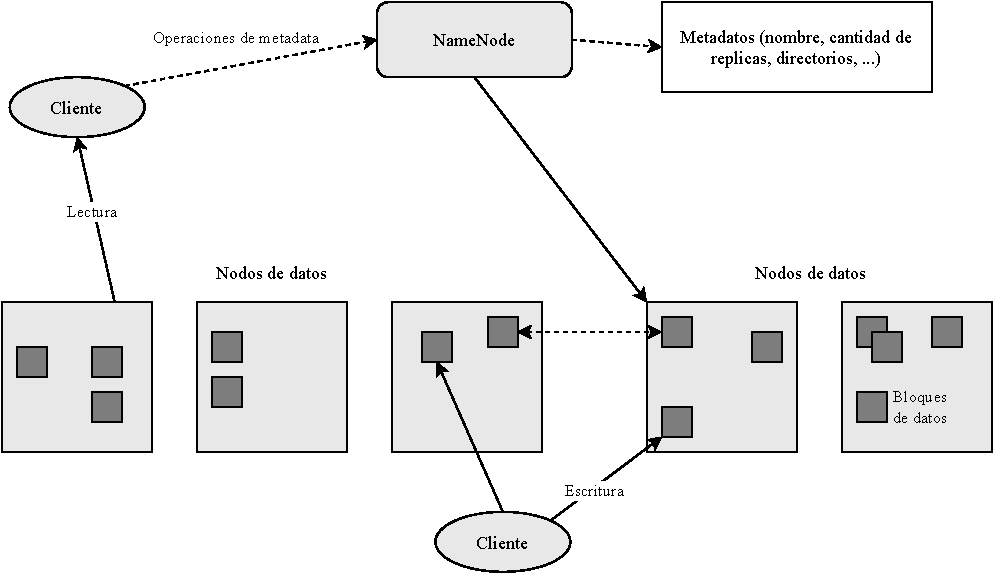
\includegraphics[width=0.9\linewidth]{7_marco_teorico/imagenes/arquitectura_hdfs}
	\caption{Arquitectura HDFS.}
	\label{fig:arquitectura_hdfs}
\end{figure}

\bigskip Tanto el NameNode como el DataNode son piezas de software diseñadas para correr, típicamente, en sistemas operativos GNU/Linux. Además, como HDFS está construido utilizando el lenguaje de programación Java, puede ser desplegado en un rango amplio de máquinas.

\paragraph{Apache Spark}
Apache Spark es una plataforma de código abierto escrita en Scala\footnote{Sitio oficial del lenguaje de programación Scala: https://www.scala-lang.org/. Último acceso: Febrero 2021.}, para procesamiento de datos a gran escala y preparado para tareas de Machine Learning iterativas \citep{meng2016mllib}. En alto nivel, una aplicación Spark consiste en un programa “driver” que ejecuta la función “main” y varias operaciones en paralelo en un cluster de computadoras\footnote{Red de computadoras de alta velocidad que se comportan como si fuesen un único servidor. No confundir con la definición de “cluster” en algoritmos de clustering.}.

\bigskip El paralelismo en un cluster de computadoras realizado por Spark se basa en particiones de datos, por ejemplo, si se desea procesar un conjunto de datos de un millón de registros y se cuenta con un cluster de 4 nodos (sin contar el nodo principal), cada uno de ellos procesará 250.000 registros. Para conseguir esto de una forma que pueda ser entendible para un desarrollador, la plataforma cuenta con una abstracción de datos llamada RDD o \textit{Resilient Distributed Dataset} (o conjunto de datos distribuido resiliente), la cual es una colección de datos particionados a través de los nodos de cluster que pueden operar en paralelo. Los RDDs son creados desde un archivo HDFS o una colección Scala existente en el programa driver. También es posible almacenarlos en memoria, permitiendo que estas colecciones sean reusadas eficientemente entre operaciones paralelas.

\bigskip Los RDDs permiten dos tipos de operaciones: \textit{transformaciones}, las cuales crean un conjunto de datos desde uno existente, y \textit{acciones} u \textit{operaciones terminales}, que devuelven un valor al programa driver luego de ejecutar una cierta cantidad de cómputos en el conjunto de datos. Estas operaciones se condicen con el modelo de programación map-reduce en el cual se basa Hadoop. Por ejemplo, map es una transformación que opera en cada uno de los elementos del conjunto de datos y devuelve un nuevo RDD representando los resultados. Por otro lado, reduce es una operación que agrega todos los elementos de un conjunto de datos usando alguna función y devolviendo un resultado final.

\bigskip Todas las transformaciones son \textit{lazy}, esto es, secuencias de acciones imperativas las cuales son retrasadas hasta que el resultado es requerido \citep{launchbury1993lazy}, es decir, las transformaciones aplicadas a un conjunto de datos son recordadas hasta que es necesario devolver un resultado final al programa driver. Además, es posible almacenar un RDD en memoria (o disco rígido) logrando así mantener elementos disponibles en un cluster para un acceso rápido en caso de que una transformación sea requerida más de una vez.
\subsection{Medidas de distancia de texto}
\subsubsection{Conceptos básicos}
\paragraph{Information retrieval}
\textit{Information retrieval} (IR) se define como encontrar material (generalmente documentos) de una naturaleza desestructurada (generalmente texto) que satisfaga una necesidad de información de grandes colecciones (generalmente almacenadas en computadoras) \citep{schutze2008introduction}.

\bigskip El IR utiliza técnicas probabilísticas, pero también, en los últimos años, investigadores se han centrado en técnicas basadas en conocimiento. Estas últimas, han hecho una significante contribución al IR “inteligente”. Más recientemente, la investigación se ha volcado a nuevas técnicas de aprendizaje inductivo basadas en \textit{inteligencia artificial} (IA), las cuales incluyen redes neuronales, aprendizaje simbólico y algoritmos genéticos \citep{chen1995machine}. Cuando hablamos de aprendizaje, nos referimos a un fenómeno multifacético. Los procesos de aprendizaje incluyen la adquisición de un nuevo conocimiento declarativo, la organización del nuevo conocimiento, representaciones efectivas, y un descubrimiento de nuevos hechos y teorías a través de la observación y la experimentación. Desde el nacimiento de la era de las computadoras, estas capacidades han querido ser implantadas en las mismas. El estudio y el modelado en computadoras del proceso de aprendizaje en múltiples manifestaciones constituyen el propósito principal del Machine Learning \citep{mitchell2013artificial}.

\bigskip Los Sistemas de Recomendación a los cuales se hace foco en este trabajo, aplican técnicas que no son más que conceptos derivados de IR y algunos de ML. Técnicas probabilísticas y determinísticas son utilizadas para extraer información relevante desde diferentes orígenes de datos, así como también generar información valiosa a partir de ellos. Para este último propósito, se han desarrollado métodos basados en el aprendizaje inductivo que demostraron ser muy efectivos y, en algunos casos, fueron útiles para modelos simples y aplicables que permiten desarrollar RSs eficaces y escalables.

\paragraph{Unidad de documento}
Una \textit{unidad de documento}, es una secuencia de caracteres de longitud fija con las cuales se va a trabajar. Estas secuencias de caracteres pueden estar codificadas por uno o varios bytes o esquemas de codificación multibyte, como UTF-8 o varios estándares específicos de algún país o compañía. Una vez que la codificación esté determinada, se debe decodificar la secuencia de bytes a una secuencia de caracteres.

\paragraph{Stopwords}
En informática, se llama stopword a una palabra que se filtra antes o después del procesamiento de datos del lenguaje natural \citep{leskovec2014mining}. Generalmente, este tipo de palabras son extremadamente comunes, y podrían tener poco valor en el momento de seleccionar documentos que coincidan con las necesidades de un usuario \citep{schutze2008introduction}.

\bigskip Entonces, es necesario seleccionar una lista de stopwords, que serán filtradas en el procesamiento de las unidades de documento. Estas listas son llamadas \textit{stop lists}. La estrategia general para el armado de stop lists, es ordenar los términos por \textit{collection frequency}, es decir, el número total de veces que aparece un término en la colección de documentos. Una vez hecho esto, es necesario tomar los términos más frecuentes, a veces filtrados a mano según su contenido semántico relativo al dominio de los documentos que están siendo indexados.

\paragraph{Tokenización}
Dado una secuencia de caracteres y una unidad de documento definida, la \textit{tokenización} es la tarea de dividirla en distintas piezas, llamadas \textit{tokens} y, quizás en el mismo momento, desechar ciertos caracteres (como signos de puntuación). Un ejemplo de tokenización de una secuencia de caracteres en idioma inglés, podría ser:

\begin{verbatim}
Input: Friends, Romans, Countrymen, lend me your ears;
Output: [Friends] [Romans] [Countrymen] [lend] [me] [your] [ears]
\end{verbatim}

Estos tokens, son frecuentemente confundidos con palabras, pero es importante hacer la distinción entre \textit{token}, \textit{tipo}, y \textit{término}, para comprender la diferencia. Un token es una instancia de una secuencia de caracteres en un documento en particular que están agrupados juntos como una unidad semántica útil para procesamiento. Un tipo es la clase de todos los tokens que contienen la misma secuencia de caracteres. Un \textit{término} es un tipo, que es incluido en un diccionario de un sistema de IR. Por ejemplo, si un documento a ser indexado es “to sleep perchance to dream”, existen 5 tokens, pero solo 4 tipos (ya que hay dos instancias del token “to”). Sin embargo, si “to” es desechada por ser un stopword, habrá entonces 3 términos: “sleep”, “perchance” y “dream”.

\paragraph{Similaridad}\label{paragraph:similaridad}
Es de interés poder cuantificar la relación entre los objetos de texto. Existen distintas maneras de medir esa relación. En general se habla de medidas de proximidad \citep{xu2008clustering}. Las medidas de proximidad son una generalización para las medidas de similaridad y disimilaridad. En este trabajo utilizaremos medidas de similaridad comúnmente encontradas en la literatura \citep{resnik1995using, lin1998information, gomaa2013survey, harispe2015semantic}. Debido al propósito de este trabajo, es de interés, en particular, la similaridad semántica en taxonomías \citep{resnik1995using}, que se basa en el contenido de información de las unidades documentales.

\bigskip Las medidas basadas en contenido de información de una unidad de documento (o concepto) en una taxonomía, utilizan el siguiente enfoque.  Se define \(p(t)\) como la probabilidad de un concepto \(t\), formalizando:
\[p(t)=\frac{freq(t)}{N}\]
donde \(freq(t)\) es la frecuencia que aparece un concepto, teniendo en cuenta el concepto en sí y todos sus antecesores; y \(N\) la cantidad total de conceptos en el corpus. De esta forma, el nodo raíz tendrá \(p(t) = 0\), mientras los nodos hojas, tendrán valores cercanos a 1. Se define el contenido de información \(I(t) = 0\) como:
\[I(t)=-\log p(t)\]

Aplicando el logaritmo negativo a \(p(t) = 0\) se logra que los nodos hoja, siendo conceptos muy específicos, contengan mucha información, y que los nodos más genéricos que se encuentran cerca de la raíz posean un contenido de información que, por lo contrario, tienda a cero.

\bigskip \cite{resnik1995using} define, en un conjunto de conceptos \(C\) en una taxonomía \textit{es-un} que permite herencia múltiple, que la similaridad entre dos conceptos es la medida en que ellos comparten información en común, indicado, en este tipo de taxonomías, por el nodo inmediato de más alto nivel que los subsume a ambos, el \textit{subsumidor mínimo} (minimum subsumer o ms por sus siglas en inglés).

\bigskip Considerando dos términos \(t_i\) y \(t_j\), y a \(S(t_i, t_j)\) al conjunto de ancestros comunes de \(t_i\) y \(t_j\), se define al subsumidor mínimo, \(ms(t_i, t_j)\), como al término de \(S(t_i, t_j)\) que contiene el máximo contenido de información:
\[\max_{t \in s(t_i,t_j)} I(t) = I(ms(t_i,t_j))\]

La medida de similaridad de \cite{resnik1995using} \(S_R\), es entonces, el contenido de información del subsumidor mínimo de dos términos:
\[S_R = I(ms(t_i,t_j))\]

El enfoque anterior, posee la siguiente particularidad: no tiene en cuenta la similaridad de los nodos con respecto a su subsumidor mínimo. Es intuitivo pensar que dos conceptos abstractos (nodos ubicados en posiciones más cercanas al subsumidor mínimo) son más parecidos entre sí que dos conceptos específicos (más alejados del subsumidor mínimo) \citep{lin1998information}. Para solucionar esto, \cite{lin1998information} tiene en cuenta dos aspectos para calcular la similaridad entre dos conceptos en este tipo de taxonomías: \begin{enumerate*} [label=(\roman*)] \item La cantidad de información; y \item La ubicación relativa entre los nodos hijos respecto al subsumidor mínimo.\end{enumerate*} Definida como la similaridad de \cite{resnik1995using}.

\bigskip La medida de Lin es:
\[S_L(t_i, t_j)=\frac{2S_R(t_i,t_j)}{I(t_i)+I(t_j)}\]

El resultado de esta medida, estará normalizada en el rango \([0, 1]\) y obtiene que nodos más generales, con menor cantidad de información, sean más similares entre sí, que dos nodos específicos (ya que la cantidad de información de los mismos aumentará el denominador de la ecuación, disminuyendo el resultado final). Se ha demostrado que esta definición de similaridad produce una correlación ligeramente mayor con los juicios humanos.

\paragraph{Medidas de proximidad}
Proximidad es la generalización de similaridad y disimilaridad. La función disimilaridad, también conocida como función de distancia, en un conjunto de datos X, es definida para satisfacer las siguientes condiciones. Las condiciones mencionadas, son las utilizadas por \cite{xu2008clustering} y de relevancia en el presente trabajo:

\begin{enumerate}
	\item Simetría,
	\[D(x_i,x_j)=D(x_j,x_i);\]

	\item Positividad,
	\[D(x_i,x_j) \geq 0 \quad \forall x_i,x_j;\]
\end{enumerate}

De forma, análoga la función de similaridad es definida satisfaciendo las condiciones:
\begin{enumerate}
	\item Simetría,
	\[S(x_i,x_j)=S(x_j,x_i);\]

	\item Positividad,
	\[0 \leq S(x_i,x_j) \leq 1, \quad \forall x_i,x_j\]
\end{enumerate}

Si bien el término matemático de distancia exige una serie de supuestos rigurosos \citep{xu2008clustering}, en este trabajo utilizaremos la noción de distancia y de disimilaridad en forma indistinta, y nos basaremos en las medidas de proximidad habitualmente utilizadas para comparación de texto. Por lo tanto, para transformar una medida de similaridad \(S(x_i,x_j)\) en una de distancia \(D(xi,xj)\) que cumpla \(0 \leq D(x_i,x_j) \leq 1\), haremos la normalización de la misma en el intervalo \([0,1]\) y luego aplicaremos el cálculo \(D(x_i,x_j) = 1 - S(x_i,x_j)\) y recíprocamente \citep{leale2013novel}.

\paragraph{Modelo de espacio vectorial}
En el modelo de espacio vectorial, un texto es representado como un vector de términos. Si las palabras son elegidas como términos, entonces cada palabra del vocabulario sería una dimensión independiente en el espacio vectorial \citep{singhal2001modern}. Todo texto puede ser representado por un vector en este espacio dimensional. Si un término pertenece a un documento, este obtiene un valor distinto de cero en el vector, junto con la dimensión correspondiente al término. Como un documento contiene un conjunto limitado de términos (el vocabulario puede contener millones de términos), muchos de los vectores pueden ser muy dispersos. La mayoría de los sistemas basados en vectores trabajan en el cuadrante positivo, es decir, a ningún término se le asigna un valor negativo.

\bigskip Para asignar un valor numérico a un documento en una consulta, el modelo mide la similaridad entre el vector ingresado en ella y el vector del documento al cual se quiere consultar. La similaridad entre dos vectores no es inherente al modelo. Típicamente, el ángulo entre los dos vectores es usado como medida de divergencia entre los mismos, y el coseno del ángulo es usado como similaridad numérica, ya que el coseno tiene la propiedad de ser tener resultado 1 cuando los vectores son idénticos y 0 cuando los vectores son ortogonales (explicado en detalle más adelante). Como una alternativa, el producto escalar entre dos vectores, es también usado como medida de similaridad. Si todos los vectores están forzados a tener longitud 1, es decir, vectores unitarios, entonces el coseno del ángulo entre los vectores, tiene el mismo resultado que el producto escalar.

\bigskip Formalizando, si \(\overrightarrow{D}\) es el vector del documento y \(\overrightarrow{Q}\) es el vector de la consulta, la similaridad entre \(\overrightarrow{D}\) y \(\overrightarrow{Q}\) es representada como:
\[S(\vec{D},\vec{Q})=\sum_{ti \in Q,D}^{ }{W_{t_{iQ}}.W_{t_{iD}}}\]

donde \(W_{t_{i \overrightarrow{Q}}}\) es el valor de la componente número \(i\) del vector \(\overrightarrow{Q}\) y \(W_{t_{i \overrightarrow{D}}}\) es el valor de la componente número \(i\) del vector \(\overrightarrow{D}\), también definido como el peso del término \(i\) en el documento \(D\). Cualquier término no presente en la consulta o en el documento tendrá valor cero en \(W_{t_{i \overrightarrow{Q}}}\) o \(W_{t_{i \overrightarrow{D}}}\), por lo cual es posible hacer la sumatoria solo de los términos en común entre la consulta y el documento.

\paragraph{Distancia del coseno}
La \textit{distancia del coseno} puede ser la que se aplica en mayor frecuencia en términos de similaridad en IR \citep{korenius2007principal}. Al aplicar la distancia del coseno se obtiene un resultado que se encuentra en el rango \([-1, 1]\). El valor \(-1\) significa que los vectores tienen la misma dirección, pero sentidos opuestos. El valor \(1\), por lo contrario, significa que el ángulo comprendido entre los vectores es cero.

\bigskip Particularmente en IR, es de interés el intervalo \([0, 1]\) ya que todos los componentes de un vector que representa a un documento, son no negativos. De esta interpretación, se deriva la definición de la distancia del coseno, restando la medida del coseno de su máximo valor:
\[d_c(\vec{D}_i, \vec{D}_j) = 1 - cos(\vec{D}_i, \vec{D}_j) = 1 - \frac{{\vec{D}_i}'\vec{D}_j}{\sqrt{{\vec{D}_i}'\vec{D}_i}\sqrt{{\vec{D}_j}'\vec{D}_j}}\]

donde \(i \leq i,j \leq n\). Los símbolos \(\overrightarrow{D_i}\) y \(\overrightarrow{D_j}\) son documentos en forma de vectores y \(d_c\) es la distancia entre ellos.

\bigskip Para simplificar, y teniendo en cuenta que estamos hablando de documentos en forma de vectores, la distancia del coseno se puede derivar de la fórmula del \textit{producto escalar} (producto punto). Siendo \(\overrightarrow{D_i}\) y \(\overrightarrow{D_j}\) dos documentos en forma de vectores, se define el producto escalar entre ellos, como:
\[\vec{D}_i.\vec{D}_j = \left \| \vec{D}_i \right \|.\left \| \vec{D}_j \right \|.cos(\theta)\]

siendo \(\left \|\overrightarrow{D_i}\right \|\) y \(\left \|\overrightarrow{D_j}\right \|\) los módulos de los vectores \(\overrightarrow{D_i}\) y \(\overrightarrow{D_j}\) respectivamente, y $\theta$ el ángulo formado entre ellos. Entonces:
\[cos(\theta) = \frac{\vec{D}_i.\vec{D}_j}{\left \| \vec{D}_i \right \|.\left \| \vec{D}_j \right \|}=\frac{\sum_{i=1}^{n}{{d_i}_i{d_j}_i}}{\sqrt{\sum_{i=1}^{n}{{d_i}_i^{2}}}\sqrt{\sum_{i=1}^{n}{{d_j}_i^{2}}}}\]

Donde \(d_i\) y \(d_j\) son los componentes de los vectores \(\overrightarrow{D_i}\) y \(\overrightarrow{D_j}\) respectivamente.

\subsubsection{Term Frequency}
También conocido en la literatura como \textit{Bag of words} (bolsa de palabras) o simplemente, de sus iniciales, bow. \textit{Term Frequency}, o TF; es una técnica donde el orden exacto de los términos es ignorado, pero se basa en el número de ocurrencia de cada uno de ellos \citep{christopher2008introduction} en un documento. Los términos anteriormente mencionados como referencia a esta técnica, se van a usar indistintamente en este documento.

\bigskip Si comparamos las frases en inglés \textit{“Mary is quicker than John”} y \textit{“John is quicker than Mary”}, desde esta perspectiva (ignorando el orden), son idénticas. Esto conlleva a ciertos problemas desde el punto de vista semántico, ya que, si bien el número de ocurrencia de términos es el mismo, el significado de las frases es opuesto. Las palabras son contadas en una \textit{bolsa}, lo cual difiere de la definición matemática de \textit{conjunto}, que no considera los elementos repetidos. Cada palabra corresponde a una dimensión en el espacio de datos resultante y cada documento corresponde a un vector compuesto por valores no negativos en cada dimensión \citep{huang2008similarity}. Con los documentos representados como vectores, se mide el grado de similaridad de dos documentos como la correlación entre los vectores correspondientes, que puede ser cuantificada como el coseno del ángulo entre ellos. Entonces, es posible obtener la distancia entre dos documentos en forma de vectores \(\overrightarrow{D_1}\) y \(\overrightarrow{D_2}\) aplicando:
\[d(\vec{D}_1, \vec{D}_2) = 1 - \frac{\vec{D}_1 \vec{D}_2}{\left \| \vec{D}_1 \right\| \left \| \vec{D}_2 \right\|}\]

\subsubsection{Term Frequency/Inverse Document Frequency}
Hasta ahora, no se ha mencionado que implicancia tiene la frecuencia de cada término en uno o varios documentos de una colección. Se define \textit{document frequency} \(df_t\) como el número de documentos en una colección que contienen el término \(t\), en contraste con TF que indica que tan frecuentemente aparece un término en un documento dado. El propósito de este indicador, es discriminar a nivel documento para asignar un peso a cada uno de los términos existentes en la colección de documentos \citep{christopher2008introduction}, para lo cual se define \textit{inverse document frequency}, o IDF; un indicador basado en la cantidad de documentos que contienen (o son indexados por) un término en cuestión \citep{robertson2004understanding}. La intuición se basa en que si un término de búsqueda se encuentra en muchos documentos, no es un buen discriminador, y se le debe asignar menor peso que a un término que se encuentra en pocos documentos.

\bigskip Este método, conocido como \textit{Term Frequency/Inverse Document Frequency} (TF-IDF), está basado en multiplicar la medida IDF con la medida TF. Asumiendo que existen \(N\) documentos en una colección, y un término \(t_i\) aparece en \(n_i\) documentos (\(df_t\)), entonces la medida IDF propuesta es \citep{sparck1972statistical}:
\[idf(t_i) = \log{\frac{N}{n_i}}\]

Palabras con alto valor TF-IDF implican una fuerte relación con el documento en el cual aparecen, es decir, que TF-IDF mide la relevancia de un término en un documento dado. Estas palabras, que son comunes solo en un documento o en un pequeño grupo de ellos, tienden a tener un valor TF-IDF más grande que palabras comunes como artículos y preposiciones \citep{ramos2003using}.

\bigskip El procedimiento formal para implementar TF-IDF tiene algunas diferencias menores entre diferentes aplicaciones, pero básicamente consiste como se indica a continuación. Siendo \(t_i\) un término que se encuentra en un documento \(d_j\), se calcula:
\[tfidf(t_i, d_j) = tf(t_i, d_j) \cdot idf(t_j)\]
\[tfidf(t_i, d_j) = tf(t_i, d_j) \cdot \log{\frac{N}{n_j}}\]

Esta fórmula deriva en distintos valores que puede tomar el resultado final. Teniendo en cuenta cada uno de los parámetros involucrados, se van a analizar algunas variaciones. Consideremos en principio que \(N \cong n_j\), es decir que el término \(t_i\) aparece en casi todos los documentos. Esto implica que \(1 <  \log(\frac{N}{n_j}) < c \) para un \(c\) con un valor pequeño y el valor de TF-IDF será menor que el valor de IDF, pero aún positivo (ya que \(0 \leq tf(t_i,d_j) \leq 1\)). Esto implica que el término \(t_i\) es relativamente común entre todos los documentos pero aún posee cierta importancia sobre \(N\). Este puede ser el caso de palabras muy comunes en documentos, como pronombres o preposiciones, las cuales no tienen ningún significado relevante por sí mismas, y recibirán un valor TF-IDF muy bajo. Finalmente, supongamos que el valor TF es alto, y \(n_j\) es un número pequeño. Entonces \(\log(\frac{N}{n_j})\) será bastante grande y así también lo será el valor total TF-IDF. Este último caso es en el cual estamos interesados, ya que las palabras con alto TF-IDF implica que son importantes en \(n_j\) pero no son comunes en la totalidad de los documentos. Este término \(t_i\) se dice que tiene un gran \textit{poder discriminatorio}.

\bigskip TF-IDF es un algoritmo eficiente y simple para medir el peso que tiene una palabra en una consulta para un conjunto de documentos que son relevantes para esa consulta. Además, TF-IDF es simple de codificar, sentando las bases para algoritmos más complicados y sistemas de IR. Más allá de esas fortalezas, TF-IDF tiene sus limitaciones. En cuanto a sinónimos, no hace ninguna relación entre palabras. Es decir, que no considerará documentos en los cuales la palabra no se encuentra pero si se encuentra un sinónimo de la misma, ya que las palabras son tomadas como conceptos totalmente diferentes. El mismo problema ocurre cuando se trata de plurales o una variación del tiempo verbal de una palabra, por ejemplo, “país” y “países” serán categorizadas separadas, en lugar de categorizarlas como una sola palabra y calcular un valor TF-IDF más bajo.

\subsubsection{Word2Vec}
\textit{Word2Vec} (W2V) presenta dos modelos basados en redes neuronales para computar representaciones de palabras como vectores continuos en grandes conjuntos de datos. La calidad de la representación es medida como similaridad \citep{mikolov2013efficient}. La forma de representar los vectores está basada en su contexto, el cual es usado para optimizar la representación del vector, es decir, palabras con significado similar son representadas con vectores que están más cerca unos de otros. Esto indica que, por primera vez en las medidas analizadas en el estado del arte de este trabajo, W2V toma un enfoque semántico.

\paragraph{Motivación de Word2Vec}
Muchos sistemas de \textit{procesamiento de lenguaje natural} (NLP por sus siglas en inglés correspondientes a Natural Language Processing), tratan a las palabras o unidades atómicas y no tienen noción de similaridad entre las palabras. Este tipo de sistemas son limitados para varias tareas, ya que no proporcionan información sobre las relaciones que pueden existir entre las distintas entidades. Con el progreso del Machine Learning en los últimos años, ha sido posible entrenar modelos más complejos con grandes conjuntos de datos, y en ellos se observa un rendimiento mejor que en los modelos más simples. Probablemente, el concepto más exitoso es la \textit{representación distribuida de palabras}. En estos modelos, fue descubierto que la similaridad entre palabras va más allá que simples regularidades sintácticas, por el contrario es posible realizar operaciones algebraicas entre representaciones vectoriales de palabras, tal como:

\begin{verbatim}
vector("Rey") - vector("Hombre") + vector("mujer") = vector("Reina")
\end{verbatim}

Los vectores adhieren muy bien a nuestra intuición, por ejemplo, palabras que son sinónimos tienden a tener vectores similares en términos de la distancia del coseno, mientras que antónimos, tienden a tener vectores disímiles. Por lo cual, el objetivo es maximizar la precisión de estas operaciones entre vectores mediante un arquitecturas de modelos que preserven regularidades lineales entre palabras así como también minimizar la complejidad computacional. Estos vectores son útiles por dos razones principales \citep{mccormick2016word2vec}:

\begin{enumerate}
	\item Se puede medir la similaridad semántica entre dos palabras calculando la distancia del coseno entre los vectores correspondientes.
	\item Es posible usar los vectores en distintas tareas de NLP, tales como clasificación de documentos o análisis de sentimientos.
\end{enumerate}

\bigskip Las arquitecturas propuestas por W2V se basan en dos modelos, \textit{Skip-Gram} y \textit{CBOW} (Continuous Bag of Words). Ambos modelos son simples redes neuronales con una capa oculta, y los vectores son resultados de propagación hacia atrás y \textit{descenso de gradiente estocástico} (SDG por sus siglas en inglés correspondientes a Stochastic Gradient Descent). La Figura \ref{fig:cbowskipgram} muestra la diferencia entre ambos modelos, los dos utilizando una capa oculta: a la izquierda, CBOW utiliza un conjunto de palabras y predice la palabra actual \(w(t)\); a la derecha, Skip-gram predice palabras vecinas a partir de una palabra \(w(t)\). El detalle de cada uno de los métodos es descrito a continuación.

\begin{figure}[h!]
	\centering
	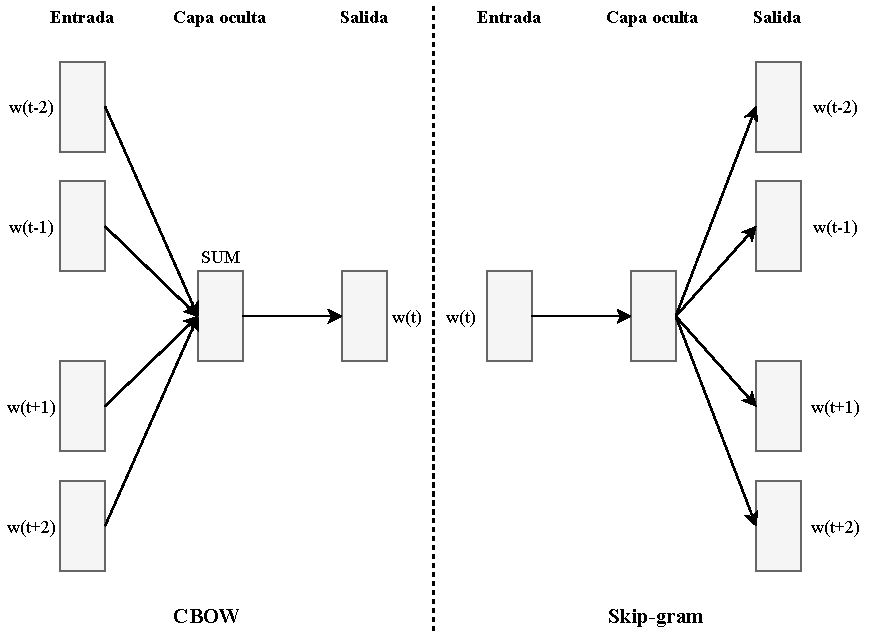
\includegraphics[width=0.7\linewidth]{7_marco_teorico/imagenes/cbow_skipgram.pdf}
	\caption{La arquitectura CBOW predice la palabra actual basándose en el contexto, mientras que la arquitectura Skip-gram predice palabras vecinas, dada una palabra como entrada \citep{mikolov2013efficient}.}
	\label{fig:cbowskipgram}
\end{figure}

\paragraph{Modelo Skip-Gram}
El modelo Skip-gram se basa en lo siguiente: dado un conjunto de frases (llamado \textit{corpus}) el modelo analiza las palabras de cada sentencia y utiliza cada palabra para predecir las palabras que serán vecinas, esta técnica se basa en la \textit{propagación hacia atrás}. La entrada para este modelo es una sola palabra \(w_I\) y la salida, su contexto \(\{w_{0,1},..., w_{0,C}\}\) definido por una ventana de tamaño \(C\). Una potencial instancia de entrenamiento podría ser la palabra “auto” como entrada y las palabras \{"Manejé","mi","hacia","la","tienda"\} las salidas. El objetivo es, mediante el entrenamiento, generar los pesos de la capa oculta de la red neuronal y usarlos como los vectores que representarán las palabras. Mediante la palabra que es usada como entrada, el modelo busca palabras “vecinas” pertenecientes a su contexto y elige una de forma aleatoria. La red neuronal dará como resultado la probabilidad de cada palabra en nuestro vocabulario de ser \textit{palabra vecina}. El concepto de palabra vecina, viene dado por el tamaño de ventana que hayamos elegido, si el tamaño de ventana es 5, significa que son tomadas en cuenta 5 palabras adelante y 5 palabras atrás (10 en total) \citep{skipgrammodel}.

\bigskip La entrada de la red neuronal será una palabra representada como \textit{one-hot vector}, un vector con tantas posiciones como tamaño tenga el vocabulario; esto es, si tenemos un vocabulario de 10000 palabras, el vector tendrá el valor 1 en la posición donde se encuentre la palabra representada, y 0 en las 9999 restantes. La salida de la red neuronal, es otro vector con las mismas 10000 posiciones, que en cada posición contiene las probabilidades de que cada una de las palabras sean vecinas de la palabra representada en la entrada. Las probabilidades son calculadas de la siguiente forma. Dado un one-hot vector \(x\) de tamaño \(V\) (cantidad de palabras del vocabulario) correspondiente a la palabra de entrada, y un conjunto de redes neuronales de la capa oculta de tamaño \(N\). Dado una ventana de tamaño \(C\), tendrémos \(\{y_1,...,y_C\}\) vectores one-hot correspondientes a las palabras de salida en la instancia de entrenamiento. La matriz \(W=V \times N\) es la matriz de pesos entre la capa de entrada y la capa oculta, cuya fila \(i^{th}\) representa los pesos correspondientes a la palabra \(i^{th}\) del vocabulario. Esta matriz \(W\) contiene entonces, la codificación como vector de cada una de las palabras del vocabulario (como filas), las cuales serán entrenadas mediante la red neuronal. El siguiente ejemplo ilustra, cómo la matriz \(W\) multiplicada por el vector de entrada, resulta en el vector que la representa.
\[\begin{bmatrix}0 & 0 & 0 & 1 & 0 \end{bmatrix} \times  \begin{bmatrix}12 & 14 & 2 \\ 6 & 19 & 74 \\ 22 & 33 & 96 \\ 36 & 85 & 2 \\ 95 & 1 & 56 \end{bmatrix} = \begin{bmatrix} 36 & 85 & 2 \end{bmatrix}\]

Se puede ver, cómo el vector resultado de tamaño \(1 \times N\) es la 4 fila de la matriz \(W\), ya que la palabra de entrada es un vector one-hot con el valor \(1\) en el cuarto elemento.

\bigskip Una vez obtenido el vector de salida, éste es usado como entrada para la capa de salida de la red neuronal, usando un clasificador de regresión Softmax \citep{morin2005hierarchical}, el cual es una generalización de la regresión logística para el caso en que se quieren manejar múltiples clases\footnote{Tutorial en profundidad de regresión Softmax \url{http://ufldl.stanford.edu/tutorial/supervised/SoftmaxRegression},  Último acceso: Febrero 2021.}. Cada una de las \(V\) neuronas de la capa de salida, producirá un valor entre \(0\) y \(1\). Además, la suma de todos estos valores, será \(1\), es decir, una distribución de probabilidades. Específicamente, cada neurona de salida tiene un vector de pesos correspondiente a cada una de las palabras del vocabulario, que se multiplica con el vector que proviene de la capa oculta y se aplica una función Softmax. El resultado es la probabilidad de que aleatoriamente se seleccione la palabra de entrada y sea vecina a cada una de las palabras representadas por los vectores en las neuronas de salida.

\paragraph{Modelo Continuous Bag of Works (CBOW)}
Es similar al modelo Skip-gram pero con las salidas y las entradas invertidas: dado un conjunto de palabras que definen un contexto, CBOW predice la palabra actual. La capa de entrada consiste en \(C\) palabras del contexto, codificadas como vectores one-hot, es decir un conjunto \( \{x_1,..., x_C\}\) cada uno de dimensión \(V\). La capa oculta es un vector \(h\) de tamaño \(N\). Finalmente, la salida es una palabra \(y\) también codificada como un vector one-hot. Los vectores de entrada son conectados con la capa oculta por una matriz \(W=V \times N\), y esta capa oculta a su vez es conectada con la capa de salida vía otra matriz \(W'=V \times N\) \citep{cbowmodel}.

\bigskip La salida de la capa oculta \(h\) de la red neuronal es el promedio de los vectores de entrada, ponderados por la matriz \(W\).
\[h = \frac{1}{C}W \cdot (\sum_{i=1}^{C}{x_i})\]
Este cómputo es una de las diferencias principales con el modelo Skip-gram. Luego, se calculan las entradas de cada nodo de la capa de salida.
\[u_j = {v'_{w_j}}^{T} \cdot h\]
donde \(v'_{w_j}\) es la \(j^{th}\) columna de la matriz \(W'\). Y finalmente se calcula el resultado de la capa de salida. Dicha salida \(y_j\) es obtenida pasando la entrada \(u_j\) por la función Softmax.
\[y_j=p(w_{y_j}|w_1,...,w_C)=\frac{exp(u_j))}{\sum_{V}^{j=1}exp(u_j')}\]

\bigskip Entonces, la capa de salida es una palabra \(y_j\) codificada como un vector one-hot de dimensión \(V\).

\subsubsection{FastText}
Fastext\footnote{Sitio de FastText \url{https://fasttext.cc}. Último acceso: Febrero 2021.} es una librería open-source que permite generar representaciones de texto y clasificadores de texto. Está basada en una técnica representación continua de palabras, que tiene en cuenta la morfología\footnote{Parte de la lingüística que estudia las reglas que rigen la flexión, la composición y la derivación de las palabras. Por ejemplo, las distintas conjugaciones de los verbos en español.} de las mismas \citep{bojanowski2017enriching}.
El modelo de FastText está basado en el modelo Skip-gram, donde cada palabra es representada como una bolsa de caracteres \(n-gramas\). Y a cada uno de los n-gramas, se le asignará un vector, que luego, sumados, representarán cada palabra. Dos características muy importantes son, \begin{enumerate*} [label=(\roman*)] \item el método es muy rápido, permitiendo entrenar grandes conjuntos de datos; y \item permite calcular representación de palabras que no aparecen en el conjunto de entrenamiento.  \end{enumerate*}

\bigskip Repasando el modelo Skip-gram, introducido por \cite{mikolov2013efficient}, dado un vocabulario \(V\), donde una palabra es identificada por su índice \(w \in \{1,... , V\}\) , el objetivos es aprender la representación vectorial de cada palabra \(w\). Dado un documento grande representado como una secuencia de palabras \(w_1, ..., w_t\), el objetivo del modelo Skip-gram es que las representaciones de las palabras sean entrenadas para \textit{predecir bien} otras palabras que aparecen en el contexto, es decir, minimizar la siguiente probabilidad logarítmica:
\[\sum_{t=1}^{T}\sum_{c \in C_t}^{T}{\log p(w_c | w_t)}\]
donde el contexto \(C_t\) es el conjunto de índices de palabras que están alrededor de \(w_t\).

\paragraph{Modelo sub-palabra}
Usando una representación en forma de vector para cada palabra, se ignora la estructura interna de las mismas. El modelo sub-palabra, propone una función de scoring \(s\), con el objetivo de tener en cuenta esta información.
Cada palabra \(w\) es representada como una bolsa de n-gramas. Se agregan los símbolos ``\(<\)'' y ``\(>\)'' para delimitar el principio y el final de cada palabra. También, se incluye la palabra en sí misma como otro n-grama. Por ejemplo, la palabra ``where'' y con un \(n = 3\) (longitud de la sub-palabras, en este caso sería, tri-gramas), obtenemos:

\begin{center}\ttfamily\sbox{0}{a}%
	\begin{minipage}{45\wd0}% 45 characters here
		\begin{verbatim}
		'<wh', 'whe', 'her', 'ere', 're>' y '<where>'
		\end{verbatim}
	\end{minipage}
\end{center}

Cabe aclarar que los símbolos ``\(<\)'' y ``\(>\)'' también son considerados como caracteres a la hora de construir los n-gramas. Por ejemplo, ``\(<wh\)'' es un trigrama con un delimitador de inicio de palabra.

\bigskip Dado un diccionario de n-gramas de tamaño \(G\) y una palabra \(w\), el conjunto de n-gramas que aparecen en \(w\) es \(G_w \in \{1,..., G\}\). Se asocia un vector \(z_g\) a cada n-grama \(g\). Se representa una palabra, como la suma de todas las representaciones vectoriales de sus n-gramas. Entonces, la función scoring, es:
\[s(w,c) = \sum_{g \in G_w}^{}{}z_g^T v_c\]

Este modelo, permite compartir las representaciones entre las palabras y, también, aprender una representación confiable de palabras extrañas o poco frecuentes.

\subsubsection{Semantic Distance}
La \textit{distancia semántica} usada en este trabajo está basada en redes semánticas y estadísticas de corpus \citep{li2006sentence}. El método en cuestión está basado en el cálculo de similaridad entre textos de distancia corta, que tiene en cuenta la información semántica y la información del orden de las palabras implicadas en las frases involucradas. La información semántica de las frases es obtenida desde una base de datos léxica y \textit{estadísticas de corpus}\footnote{El estudio de los aspectos estadísticos de los textos se ha centrado tradicionalmente en el análisis de la frecuencia de los elementos y fenómenos que se encuentran en ellos, especialmente en lo referido al componente léxico.}. El uso de una base de datos léxica posibilita modelar el sentido común humano y las estadísticas de corpus adaptar el método a diferentes dominios.

\bigskip Uno de los puntos dominantes por el cual este método es particularmente efectivo para calcular similaridad entre frases cortas se basa en que, tradicionalmente los métodos basados en palabras comunes funcionan bien solo para textos largos, para los cuales existe una alta posibilidad de que una palabra se encuentre en los documentos en comparación. En cambio, para textos cortos, la coocurrencia de palabras entre ellos es muy rara o nula. Esto se debe a la flexibilidad de los lenguajes de expresar mismos significados usando diferentes frases en términos de estructura y palabras.

\paragraph{El método}
\begin{figure}[h!]
	\centering
	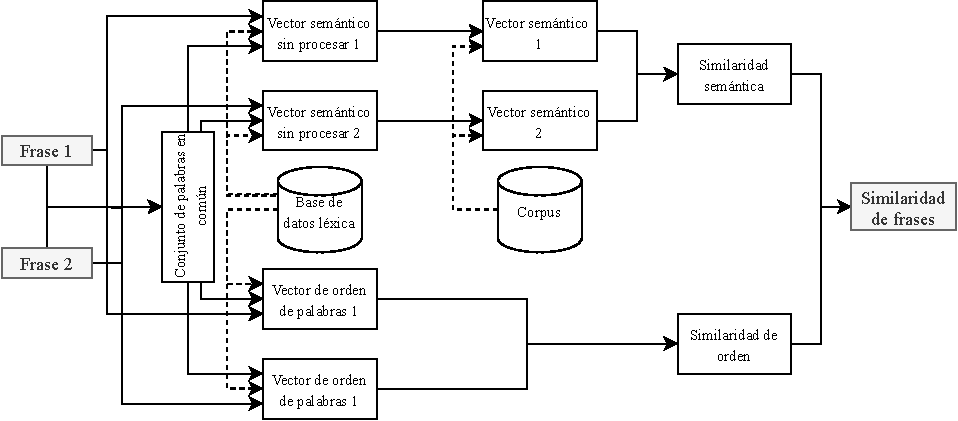
\includegraphics[width=0.9\linewidth]{7_marco_teorico/imagenes/similaridad_sematinca_metodo}
	\caption{Diagrama de cálculo de similaridad semántica.}
	\label{fig:similaridadsematincametodo}
\end{figure}

El procedimiento de cálculo de similaridad entre dos frases, como se muestra en la Figura \ref{fig:similaridadsematincametodo}, utiliza un conjunto de palabras en común usando todas las palabras distintas en el par de frases (en lugar de usar un conjunto fijo como vocabulario). De cada una de las frases, un vector semántico sin procesar es derivado, utilizando la base de datos léxica. También, un vector de orden de palabras es generado a partir de cada frase utilizando la base de datos. Como cada palabra en una frase, contribuye de forma diferente al significado de la misma, la importancia de cada una de ellas es ponderada utilizando información de contenido derivado del corpus. Combinando la información de corpus con los vectores semánticos sin procesar, se obtienen nuevos vectores semánticos los cuales servirán para calcular la \textit{similaridad semántica}. Una \textit{similaridad de orden} es calculada usando los dos vectores de orden previamente generados. Finalmente, la similaridad entre frases es calculada combinando la similaridad semántica y la similaridad de orden.

\paragraph{Similaridad semántica entre palabras}
Las bases de conocimiento tienden a representar el sentido común humano con una estructura jerárquica para un dominio específico o para un lenguaje en general. Existen varios proyectos lingüísticos disponibles en la web, tales como WordNet \citep{miller1995wordnet}, Spatial Date Transfer Standard de la USGS\footnote{United States Geological Survey. https://www.usgs.gov/. Último acceso: Febrero 2021.}, y Gene Ontology\footnote{Gene Ontology. http://geneontology.org/. Último acceso: Febrero 2021.}. Esta estructura jerárquica, se puede modelar como una taxonomía de conceptos.

\bigskip Dadas dos palabras \(w_1\) y \(w_2\), es necesario encontrar la similaridad \(S(w_1,w_2)\) entre ellas. Esto es posible analizando la base de datos léxica (en este caso WordNet si se cuenta con palabras en el idioma inglés) de la siguiente forma: Las palabras están organizadas como conjuntos de sinónimos (llamados \textit{synsets}), con relaciones semánticas a otros synsets. Un método directo para calcular la similaridad es encontrar el camino más corto que conecta dos palabras. Por ejemplo, si tomamos la estructura detallada en la Figura \ref{fig:taxonomiasemantica}, la cual muestra un esquema de base de datos semántica en forma jerárquica que tiene como raíz al synset ``entidad'', el camino más corto para conectar ``niño'' y ``niña'' sería ``niño-persona masculina-humano-persona femenina-niña'', y tiene una longitud de \(4\). El synset ``persona, humano'', en este caso, es llamado \textit{subsumidor mínimo de palabras}, tal como se menciona en la sección \ref{paragraph:similaridad}, ya que sirve de anclaje entre los dos conceptos para los cuales se quiere calcular la distancia semántica.

\begin{figure}[h!]
	\centering
	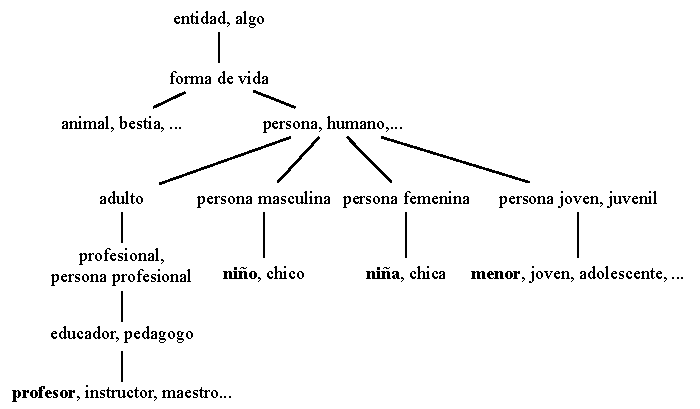
\includegraphics[width=0.9\linewidth]{7_marco_teorico/imagenes/taxonomia_semantica}
	\caption{Base de datos semántica de forma jerárquica.}
	\label{fig:taxonomiasemantica}
\end{figure}

También, se puede ver que la distancia entre ``niño'' y ``profesor'' es 6, mientras la distancia entre ``niño'' y ``animal'' es 4, lo cual es contra intuitivo e indica que el proceso es mejorable agregando más información de estas estructuras jerárquicas. Es evidente que los synsets pertenecientes a capas altas de la estructura tienen conceptos semánticos más generales y menos similaridad entre ellos, y en capas inferiores, sucede lo contrario, conceptos más particulares y similares. Lo anterior sugiere tomar en cuenta la profundidad en jerarquía. Para resumir, la similaridad entre palabras es determinada, no solo por el camino más corto entre ellas, sino también por la profundidad jerárquica, es decir:
\[S(w_1,w_2)=f(l,h)\]

donde \(l\) es el camino más corto entre \(w_1\) y \(w_2\), y \(h\) es la profundidad del subsumer de las mismas en la jerarquía de la red semántica.

\paragraph{Similaridad semántica entre frases}
Contrariamente a métodos clásicos que usan vocabularios con miles de palabras precompiladas, este método semántico usa únicamente vectores semánticos formados por las frases en comparación. Un conjunto de palabras comunes \(T\) es formado por la unión de las dos frases en comparación, luego, un vector semántico léxico es derivado. Cada entrada del vector corresponde a una palabra del conjunto de palabras comunes, lo cual indica que la dimensión del vector es igual al número de palabras del conjunto. El valor de una entrada del vector semántico es calculado de la siguiente forma:
\begin{itemize}
	\item \textbf{Caso 1}.  Si \(w_i\) aparece en la frase, \(s_i\) es 1.
	\item \textbf{Caso 2}. Si \(w_i\)  no está contenida en \(T_1\), una similaridad semántica es calculada entre \(w_1\) y cada palabra en \(T_1\) utilizando el método de la sección anterior.
\end{itemize}

Luego, es necesario ponderar cada una de las palabras basadas en su contenido de información \citep{ribadas2005semantic}. Cada celda es ponderada por la información de contenido \(I(w_i)\) y \(I(\widetilde{w}_i)\). Finalmente, el valor de la entrada del vector semántico es:
\[s_i = \check{s} \cdot I(w_i) \cdot I(\widetilde{w}_i)\]

donde \(w_i\) es una palabra en el conjunto de palabras comunes, y \(I(\widetilde{w}_i)\) es su palabra asociada en la frase. Entonces, la similaridad semántica entre dos frases es definida como el coeficiente del coseno entre los dos vectores:
\[S_s = \frac{s_1. s_2}{||s_1||.||s_2||}\]

\paragraph{Similaridad de orden entre frases}
Consideremos dos frases \(T_1\) y \(T_2\), por ejemplo:
\begin{itemize}
	\item \textbf{T1}:  A quick brown dog jumps over the lazy fox.
	\item \textbf{T2}. A quick brown fox jumps over the lazy dog.
\end{itemize}

Estas frases tienen exactamente las mismas palabras, pero dos de ellas, ubicadas en orden inverso. Como las dos frases contienen las mismas palabras, un método basado en Bag of Words, resultará en que las frases son idénticas, pero para un intérprete humano, es claro que las frases sólo son similares en cierto grado. Por lo cual, un método computacional de similaridad entre frases debe tener en cuenta el orden de las palabras. En el ejemplo, el conjunto de palabras comunes es:

\begin{center}\ttfamily\sbox{0}{a}%
\begin{minipage}{45\wd0}% 45 characters here
	\begin{verbatim}
T = {A quick brown dog jumps over the lazy fox}
	\end{verbatim}
\end{minipage}
\end{center}

Para lograr esto, este método asigna un índice único por cada palabra en \(T_1\) y \(T_2\), en orden, armando un arreglo de palabras. Un vector de orden \(r\) es formado para \(T_1\) y \(T_2\), respectivamente, basado en el conjunto de palabras comunes. Tomando \(T_1\) como ejemplo, por cada palabra \(w_i\) en \(T\), se intenta encontrar la palabra más similar en \(T_1\) de la siguiente forma:
\begin{enumerate}
	\item Si la misma palabra está presente en \(T_1\), la entrada por la palabra en \(r_1\) será el índice de la misma en \(T_1\). Caso contrario, se intenta buscar la palabra más similar \(\widetilde{w}_i \) semánticamente.
	\item Si la similaridad entre \(w_i\) y \(\widetilde{w}_i \) es mayor al umbral, la entrada de \(w_i\) en \(r_1\) es completada con el índice de \(\widetilde{w}_i \) en \(T_1\).
	\item Si las dos búsquedas anteriores fallan, la entrada de \(w_i \) en \(r_1\) es \(0\).
\end{enumerate}
Aplicando este procedimiento a las frases de ejemplo, tenemos:
\[r_1 = \left \{\;1\;2\;3\;4\;5\;6\;7\;8\;9\;\right \}\]
\[r_2 = \left \{\;1\;2\;3\;9\;5\;6\;7\;8\;4\;\right \}\]
Se propone una medida de similaridad de orden entre frases como:
\[S_r = 1 - \frac{\left \| r_1 - r_2 \right \|}{\left \| r_1 + r_2 \right \|}\]
Esto significa que la similaridad de orden de palabras es determinada por la diferencia normalizada del orden de palabras.

\paragraph{Similaridad total entre frases}
La similaridad semántica y la información sintáctica (en términos del orden de las palabras) convergen en el significado de la oración. Entonces, la similaridad total entre frases es definida como la combinación de la similaridad semántica y la similaridad del orden de palabras:
\[S(T_1, T_2)=\delta S_s + (1 - \delta)S_r\]
\[S(T_1, T_2)=\delta \frac{s_1.s_2}{\left \| s_1 \right \|\left \| s_2 \right \|} + (1 - \delta)\frac{\left \|r_1-r_2  \right \|}{\left \| r_1+r_2 \right \|}\]

\bigskip donde \(\delta \leq 1\) decide la contribución relativa de cada una de las medidas de similaridad. Como el orden de palabras cumple un rol subordinado, se recomienda que \(\delta\) tenga un valor mayor a \(0.5\).


\subsection{Ensamble de Clustering}
\subsubsection{Clustering}\label{sec:clustering}
El Clustering o \textit{análisis cluster} tiene por objetivo agrupar elementos en grupos homogéneos en función de las similitudes o similaridades entre ellos. Normalmente se agrupan las observaciones, pero el Clustering puede también aplicarse para agrupar variables. Estos métodos se conocen también con el nombre de \textit{métodos de clasificación automática o no supervisada}, o de reconocimiento de patrones sin supervisión \citep{pena2013analisis}. Con esta información de clasificación a mano, se puede inferir las propiedades de un objeto específico, basándose en la categoría que pertenece. Básicamente, los sistemas de clasificación son supervisados o no supervisados, dependiendo si asignan nuevos objetos de datos a uno o a un número finito de clases supervisadas discretas o categorías no supervisadas, respectivamente \citep{xu2008clustering}.

\paragraph{Definición de Cluster}
Los algoritmos de clustering agrupan objetos de datos (patrones, entidades, instancias, observaciones, unidades) en un cierto número de clusters (grupos, subconjuntos o categorías).

\bigskip En \citep{everittcluster} se presenta la siguiente definición: “un cluster es un conjunto de entidades que son similares, y entidades de clusters diferentes no son similares”. Claramente, esta similaridad y disimilaridad debe ser definida con un criterio significativo, tales como las medidas de proximidad comentadas anteriormente.

\paragraph{Algoritmos de Clustering}\label{sec:algoritmos_clustering}
Los algoritmos de clustering están generalmente clasificados en \textit{clustering particional} y \textit{clustering jerárquico}, basándose en la forma que se generan los clusters \citep{xu2008clustering}. Los algoritmos de clustering jerárquico encuentran clusters anidados recursivamente en un modo aglomerativo, esto es, empezando con cada uno de los puntos de datos como si fueran clusters y combinándolos con el más similar, sucesivamente, para formar de este modo una jerarquía de clusters; o bien en modo divisivo (de arriba hacia abajo --en inglés, top-down--), esto es, empezando con todos los puntos de datos en un cluster y dividiendo recursivamente cada uno de los clusters en clusters más pequeños. Los algoritmos de clustering particional intentan encontrar todos los clusters simultáneamente como una partición de datos, y no imponen una estructura jerárquica; la base matemática es simple: se parte del concepto de \textit{partición}, donde no existen subconjuntos solapados y la unión de los subconjuntos es exactamente el conjunto total. La entrada de un algoritmo jerárquico es una matriz de similaridad \(n \times n\) , donde \(n\) es el número de objetos a ser analizados por medio de clustering. Por otro lado, los algoritmos particionales puede usar tanto una matriz \(n \times d\), representando \(n\) objetos en un espacio d-dimensional, o bien, como un algoritmo jerárquico, una matriz \(n \times n\) \citep{jain2010data}.

\bigskip En este trabajo, nos centraremos en algoritmos particionales, utilizando medidas de proximidad de texto para determinar cuáles objetos (cadenas de texto) pertenecerán al mismo cluster y cuáles no. Algunos ejemplos de este tipo de algoritmo son el ampliamente utilizado \textit{k-medias} \citep{macqueen1967some}, y también el \textit{Particionamiento Alrededor de Medoids (PAM)} o \textit{k-medoids}. Este último se utilizará en este trabajo, por lo cual es descrito a continuación.

\paragraph{Particionamiento Alrededor de Medoides (PAM)}
Particionamiento Alrededor de Medoides (PAM) es un algoritmo de Clustering particional, cuyo funcionamiento es similar al del k-medias, pero en lugar de tomar un conjunto de datos aleatorio como centroides y luego, iterativamente, calcularlo como medias de los clusters, se utilizan puntos, llamados \textit{medoides}, “representativos” de un cluster, y tienen la particularidad de estar más céntricamente ubicados en el mismo \citep{rdusseeun1987clustering}. A diferencia de los centroides del algoritmo k-medias, que son vectores que pueden tomar valores arbitrarios en el espacio d-dimensional de elementos de entrada, los medoides son puntos que representan a un subconjunto de los mismos elementos. En este caso no se trabaja con otros datos fuera del conjunto de datos de entrada.

\bigskip PAM tiene dos etapas, denominadas BUILD (construcción, etapa de formación de los clusters) y SWAP (intercambio, etapa de refinamiento de la partición obtenida). Nos centraremos en la etapa BUILD, ya que será la utilizada en este trabajo:
\begin{enumerate}
	\item Establecer el medoide inicial \(m_1\) como el vector de características del conjunto de datos de entrada que minimiza la distancia a todos los demás datos en \(X\).
\[m_1 = arg \> \underset{\forall x_i}{min} \sum_{j \neq i}d(x_i,x_j),\]
donde \(d(x_i,x_j)\) es una medida de distancia genérica.
	\item Considerar un vector previamente no seleccionado \(x_i\).
	\item Considerar un vector previamente no seleccionado \(x_j\) y calcular la diferencia entre su distancia al medoide previamente seleccionado \(m_1\), y su distancia al vector \(x_i\).
	\item Calcular la Contribución \(C(x_i,x_j)\) del vector \(x_j\) a la selección del vector \(x_i\), como:
\[C(x_i, x_j) = max(d(x_j, m_1) - d(x_j, x_i), 0).\]
	\item Calcular la Ganancia total obtenida a partir de la selección del vector \(x_i\) como:
\[G(x_i) = \sum_{j} C(x_j, x_i).\]
	\item Establecer el siguiente medoide como el vector previamente no seleccionado que maximiza la ganancia total, esto es:
\[m_l = arg \> \underset{\forall i}{max} \> G(x_i).\]
	\item Repetir los pasos 2 al 6 hasta llegar a obtener \(k\) medoides.
\end{enumerate}

\bigskip El método PAM puede aceptar una matriz de distancias como entrada, lo cual lo hace adecuado para utilizar las salidas de los métodos anteriormente mencionados. Como desventaja, se puede mencionar que su complejidad temporal es cuadrática, lo que se traduce como poca eficiencia en grandes conjuntos de datos, sin embargo, se han desarrollado mejoras sobre PAM para estos problemas de desempeño \citep{kaufman2009finding}.

\subsubsection{Ensamble de clustering}
Distintos algoritmos de clustering producen distintos grupos de objetos, en forma de particiones de datos. Incluso el mismo algoritmo con distintos parámetros también produce distintos grupos de datos de salida \citep{xu2008clustering}. Además, las combinaciones de diferentes representaciones de datos que no pueden ser localizadas en un espacio dimensional, pueden generar particiones de datos completamente diferentes. El Ensamble de Clustering, propone un método para extraer clusters consistentes dadas particiones variadas de entrada.

\bigskip Dado un conjunto de datos de \(n\) objetos o patrones y \(d\) dimensiones, se aplican distintas técnicas de clustering a los mismos. Luego, usando Clustering de Acumulación de Evidencias (EAC), cada partición es vista como una evidencia independiente de organización de datos, las cuales se combinan, generando una nueva matriz de similaridad \(n \times n\) entre los \(n\) patrones. Esta matriz poseerá una similaridad para cada par de elementos que será tanto más grande cuanto más veces dichos elementos participen en el mismo cluster para las sucesivas evidencias encontradas. La partición de datos final entre los \(n\) patrones es obtenida aplicando un algoritmo de clustering en la matriz de similaridad \citep{fred2005combining}.

\bigskip Debido a la existencia de muchos algoritmos de clustering, y a la posibilidad de poder variar los mismos con distintos parámetros de entrada, es difícil encontrar un algoritmo o variación del mismo que produzca los resultados esperados, funcione con distintas formas de clusters y sea adecuado para distintos conjuntos de datos. Por otra parte, esta variabilidad puede ser aprovechada para encontrar una estructura inter-patrón que represente a todas las técnicas tenidas en cuenta como entrada. Además, este método muestra que la combinación de distintos algoritmos puede resultar en la identificación de clusters subyacentes con formas, tamaños y densidades arbitrarias.

\paragraph{Definición formal}
Dado \(X = \{x_1, x_2,... , x_n\}\) un conjunto de n objetos, y dada \(\chi = \{x_1, x_2,... , x_n\}\) como la representación de esos patrones; \(x_i\) puede ser definida por ejemplo sobre un espacio d-dimensional \(x_i \in \rm I\!R^2\), en el caso que adopte una representación vectorial, o \(X = x_{i1}, x_{i2},... , x_{im_i}\) en el caso que adopte una representación de cadena de texto, donde \(m_i\) es la longitud del mismo.

\bigskip Un algoritmo de clustering toma  como entrada y organiza los \(n\) patrones en \(k\) clusters, respondiendo a algunas medidas de similaridad entre los patrones, formando una partición de datos \(P\). Diferentes algoritmos de clustering producirán, en general, distintas particiones para el mismo conjunto de datos, tanto como en términos de número de patrones en un mismo cluster o en la cantidad de clusters. También es posible producir distintos resultados con el mismo algoritmo de clustering, ya sea, variando los parámetros de entrada o explorando distintas representaciones en los patrones \citep{fred2005combining}.

\bigskip Considerando \(N\) particiones de datos \(X\), y \(\rm I\!P\) la representación de las \(N\) particiones, definimos Ensamble de Clustering como:
\[\rm I\!P = \{P^1, P^2, ..., P^N\},\]
\[P^1 = \{C^1_1, C^1_2, ..., C^1_{k1}\},\]
\[.\]
\[.\]
\[P^N = \{C^N_1, C^N_2, ..., C^N_{kN}\},\]
donde \(C^i_j\) es el cluster número \(j\) en la partición de datos \(P_i\), la cual tiene \(k_i\) clusters, y \(n^i_j\) es la cardinalidad \(C^i_j\).

\bigskip El problema es encontrar la partición de datos “óptima”, \(P^*\), usando la información disponible en \(N\) particiones de datos \(\rm I\!P = \{P^1, P^2, ..., P^N\}\). Definimos \(k^*\), como el número de clusters en \(P^*\). Idealmente, \(P^*\) debe satisfacer las siguientes propiedades:

\begin{enumerate}
	\item Consistencia con el Ensamble de Clustering \(\rm I\!P\).
	\item Robustez con pequeñas variaciones de \(\rm I\!P\).
	\item Bondad de ajuste con información de verdad de base (verdaderos clusters o patrones), si está disponible.
\end{enumerate}

\paragraph{Acumulación de Evidencias}
La idea del Clustering de Acumulación de Evidencias es combinar los resultados de múltiples ejecuciones de clustering dentro de una misma partición de datos viendo cada uno de esos resultados como una evidencia independiente de la organización de los mismos \citep{fred2005combining}. Para realizar esto, es necesario seguir los siguientes pasos:

\subparagraph{Producir ensambles de Clustering}
Los ensambles de Clustering generalmente son producidos desde dos enfoques:
\begin{enumerate*}
	\item la elección de la representación de datos y
	\item la elección de los algoritmos de clustering o los parámetros de los mismos.
\end{enumerate*}
Ya que la representación de datos de este trabajo es fija, se va a poner énfasis en el segundo enfoque. En el segundo enfoque, es posible generar ensambles de Clustering \begin{enumerate*} [label=(\roman*)] \item aplicando diferentes algoritmos de Clustering, \item usando el mismo algoritmo pero con diferentes parámetros o inicializaciones y \item explorando diferentes medidas de similaridad entre los patrones, dado un algoritmo de Clustering.\end{enumerate*}

\bigskip Desde una perspectiva computacional, los resultados de algoritmos de Clustering son independientes, lo cual permite que sean ensamblados de forma distribuida. Además, los mismos pueden ser reusados, facilitando así un análisis de datos eficiente.

\subparagraph{Combinar evidencias}
Para poder trabajar con diferentes particiones con diferentes cantidades de clusters, se propone un nuevo mecanismo para combinar resultados que deriva en una nueva medida de similaridad entre patrones. Se supone de antemano, que los patrones que pertenecen a un cluster \textit{natural} son muy probables de ser colocados en el mismo cluster, incluso a lo largo en diferentes particiones de datos. Tomado las co-ocurrencia de pares de patrones en el mismo cluster, las \(N\) particiones de datos para \(n\) patrones, son mapeadas en una \textit{matriz de co-asociación} \(n \times n\):
\[C(i,j)=\frac{n_{ij}}{N},\]
donde \(n_{ij}\) es el número de veces que el par de patrones \((i,j)\) es asignado al mismo cluster entre las \(N\) particiones de datos.

\bigskip Entonces, el mecanismo de acumulación de evidencias mapea las particiones en el ensamble de Clustering dentro de una nueva medida de similaridad entre patrones (representada por cada elemento de la matriz de co-asociación), realizando, intrínsecamente, una transformación desde el conjunto original a la nueva representación de datos.




	\chapter*{Problema de investigación y propuesta}\label{ch:problemainvestigacion}
\addcontentsline{toc}{chapter}{Capitulo 4. Problema de investigación y propuesta}

\section*{Problema de investigación y propuesta}
\addtocounter{section}{1}
\setcounter{subsection}{0}

\subsection{Hipótesis de trabajo}
A partir del relevamiento del estado del arte se establece la hipótesis de que los algoritmos de cálculo de similaridad de texto en sitios de CQA, con el fin de participar del proceso inherente a la aplicación de Sistemas de Recomendación con gran volumen de datos, pueden ser mejorados en cuanto a medidas de rendimiento y de desempeño si se aplica un método de ensamble de clustering mediante una arquitectura Big Data apropiada.

\bigskip Por tal motivo, y como respuesta a la hipótesis planteada, se presenta el desarrollo de un nuevo método de cálculo de similaridad de texto basado en una arquitectura Big Data. Este método aprovecha las características de adimensionalidad y variabilidad de datos propias del ensamble de clustering. El método se aplica a un gran conjunto de datos reales con el fin de verificar la eficiencia y eficacia del procedimiento. Asimismo, se realiza un análisis comparativo del método presentado con los algoritmos para cálculo de similaridad de texto del estado del arte.
\subsection{Metodología de investigación}
Este trabajo comenzará con una búsqueda de material científico relacionado a RS en general, RS no personalizados basados en análisis de texto, su aplicación en sitios de CQA, un análisis de algoritmos de comparación de texto del estado del arte y su aplicación a grandes volúmenes de datos mediante métodos de ensamble de clustering y, también, una evaluación de arquitecturas de software adecuadas para un enfoque Big Data e infraestructuras acordes. Esto puede ser realizado mediante sitios o librerías digitales, tales como Google Scholar\footnote{Google Scholar: \url{https://scholar.google.com.ar}. Último acceso Febrero 2021.}, IEEExplore Digital Library\footnote{IEEExplore Digital Library: \url{http://ieeexplore.ieee.org}. Último acceso Febrero 2021.}, ScIELO\footnote{SciELO: \url{http://www.scielo.org}. Último acceso Febrero 2021.}, Harvard Library\footnote{Harvard library: \url{https://library.harvard.edu}. Último acceso Febrero 2021.} o el portal del CAICYT-CONICET\footnote{Centro Argentino de Información Científica y Tecnológica del CONICET: \url{http://www.caicyt-conicet.gov.ar/sitio}. Último acceso Agosto Febrero 2021.}, entre otros.

\bigskip Definida la hipótesis correctamente y el plan de trabajo, se iniciará el desarrollo de un software de código abierto partiendo del proyecto "text comparison"\footnote{Repositorio GitHub: \url{https://github.com/Departamento-Sistemas-UTNFRRO/text_comparison}.} perteneciente al repositorio Git del departamento de Ingeniería en Sistemas de Información de la UTN FRRo. Se importarán las piezas de software del código del proyecto del estado del arte recientemente mencionado para usarlas mediante un enfoque Big Data, con nuevas herramientas basadas en Cloud Computing, Hadoop y una arquitectura de software completamente nueva que optimice este tipo de desarrollo. Una vez que se inicie el desarrollo del proyecto, serán evaluadas distintas opciones de herramientas y entornos que se utilizarán, Esto incluye:

\begin{itemize}
	\item Lenguajes de programación y librerías inherentes al mismo.
	\item Almacenes de datos, frameworks y proyectos de terceros que puedan ser incorporados en la arquitectura Big Data.
	\item Arquitecturas de software, patrones, modelos y buenas prácticas.
	\item Infraestructura: local, distribuida en una red de computadoras físicas, o distribuida y virtualizada en la nube.
\end{itemize}

\bigskip Paralelamente al desarrollo, se identificará y documentará la nueva solución de acuerdo con los requerimientos de la Maestría en Ingeniería en Sistemas de Información, a fin de obtener un trabajo de investigación de tesis de maestría de excelencia, y acorde con los parámetros que caracterizan a la institución.

\bigskip Por último, una vez finalizado el desarrollo, se realizará un registro con los indicadores resultantes, se validará la propuesta, se explicitarán los resultados obtenidos y se elaborarán las conclusiones, a fin de abrir y/o profundizar en nuevas líneas de investigación.
\subsection{Método propuesto}
Se propone el método EQuAL (\textit{Ensemble method for community Question Answering sites based on cLustering}), que mejora la calidad y eficiencia para recomendar preguntas en un sitio de CQA. Este método está basado en una arquitectura Big Data distribuida y tiene en cuenta diversas distancias de texto, combinadas mediante un método de ensamble de clustering.

\begin{figure}[h!]
	\centering
	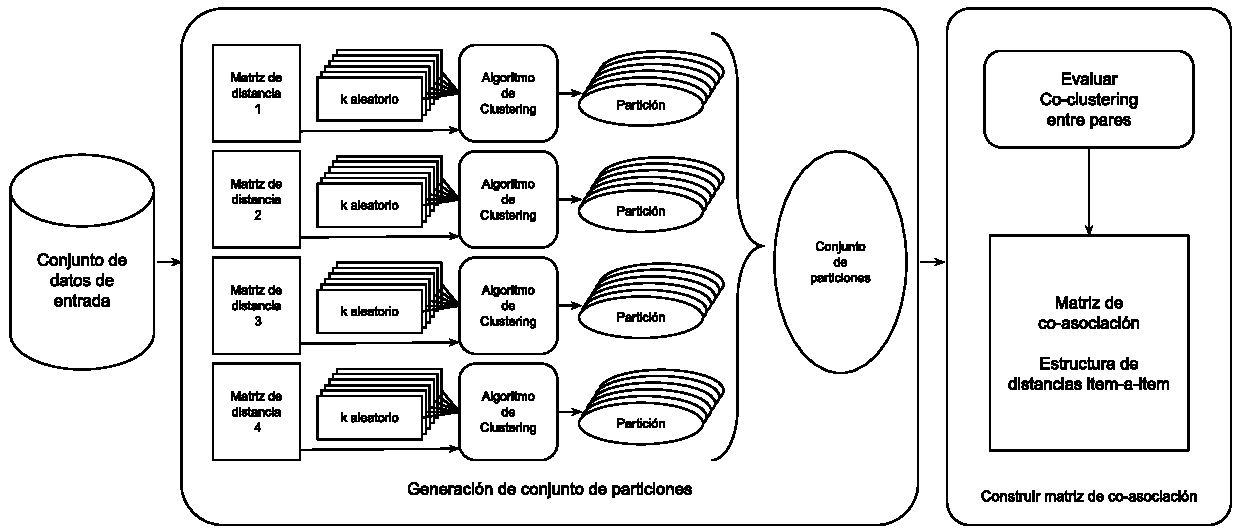
\includegraphics[width=0.9\linewidth]{8_problema_investigacion/imagenes/metodo_equal}
	\caption{Método EQuAL para la generación de matrices de co-asociación desde el conjunto de datos original.}
	\label{fig:metodoequal}
\end{figure}

 El desarrollo para este método está basado en dos pasos, como se muestra en la Figura \ref{fig:metodoequal}: \begin{enumerate*} [label=(\roman*)] \item la generación de conjunto de particiones y \item construir matriz de co-asociación. \end{enumerate*}

\subsubsection{Generación de conjunto de particiones}
El primer paso es la generación de un conjunto de particiones\(X = \{x_1, x_2,... , x_n\}\) . Cada una de las particiones será una matriz de similaridad \(x_i\). El procedimiento comenzará aplicando los distintos algoritmos de medidas de similaridad de texto del estado del arte al conjunto de datos de entrada. Por cada algoritmo, este procedimiento tendrá como resultado una matriz de similaridad. Cada una de las matrices de similaridad es el resultado de la combinación de todas las preguntas (individuales) de un muestreo original.

\bigskip Por cada matriz de similaridad, se aplicarán \(c\) corridas de algoritmos de clustering, cada uno con un número \(k\) de elementos seleccionados al azar, que es un parámetro de entrada del algoritmo de clustering, que representa el número de clusters que se generarán. Esta combinación de \(n\) matrices y \(c\) ejecuciones del proceso de clustering, resultará en \(n \times c\) salidas del algoritmo de clustering elegido, es decir, particiones \(P\) como resultado. Cada partición Pcontará con la asignación de cada pregunta individual con un cluster específico.

\bigskip Con el fin de resumir la estructura de cada una de las particiones generadas por los algoritmos de clustering, se combinan las particiones anteriormente obtenidas, dando lugar a un conjunto de particiones  \(\rm I\!P\). Específicamente, si en este método utilizamos 5 algoritmos de similaridad distintos aplicados a procedimientos de clustering, obtendremos, un conjunto de 5 particiones:
\[\rm I\!P = \{P^1, P^2, P^3, P^4, P^5\};\]
siendo 5 el número de particiones que conforman el conjunto que será la entrada del procedimiento de construcción de la matriz de co-asociación.

\subsubsection{Construcción de la matriz de co-asociación}
El segundo paso es construir una matriz de co-asociación a partir del conjunto de particiones \(\rm I\!P\). Para tal fin, se aplica un algoritmo de ensamble de clustering de acumulación de evidencias, que combinará cada una de estas particiones, dando como salida una matriz de co-asociación, que contiene en cada posición la proporción de veces que los elementos \(i,j\) caen juntos en el mismo grupo de la salida de clustering, a lo largo de las \(N=n \times c\) particiones.

\bigskip La matriz de co-asociación, que es una representación integrada de las relaciones subyacentes entre los datos originales, será la entrada para RS en sitios CQA. Además, tiene la característica de ser adimensional y comprende toda la variabilidad propia de los algoritmos de clustering, por lo cual, analiza la estructura de distancia item-item que es necesaria como entrada para un RS basado en contenido incorporando varios aspectos de las distancias entre elementos de texto, en lugar de usar solo una simple medida basada individualmente en aspectos de cada una de las medidas de distancia.

\bigskip El armado de matrices, la combinación de las mismas y la aplicación de estrategias estadísticas, implica un aumento significativo del volumen de datos y requiere una capacidad de cálculo intensiva. Una arquitectura Big Data que realice el procesamiento distribuido de los mismos es fundamental para este proceso. Además del volumen de datos con el cual se trabajará, se variarán distintos parámetros, tales como la medida de similaridad y valores de umbral involucrados en procesos de clustering, con el fin de obtener resultados confiables; lo cual redunda en múltiples ejecuciones de toda la solución. Debe destacarse que, en un primer momento, se implementarán experimentos basados en una infraestructura MapReduce aplicados con frameworks basados en Hadoop y cluster computing, desplegados en servidores elásticos en la nube, lo cual provee la ventaja de procesar grandes cantidades de datos en instancias dinámicamente escalables.

\subsection{Arquitectura de procesamiento de datos}

El procesamiento de datos se realizará con una infraestructura que permita el procesamiento distribuido en un cluster de computadoras, posibilitando que las operaciones de cómputo intensivo (ya sea calculo de distancia o ensambles de clustering) se realicen en distintos nodos al mismo tiempo. El conjunto de datos de entrada será convertido a una colección distribuida y dividida en \(P\) particiones de datos. Cada una de esas particiones será asignada a un nodo del cluster, que realizará el cálculo de distancia con un algoritmo determinado. La Figura \ref{fig:equaldistribuido} muestra los componentes y procesos involucrados en la arquitectura de procesamiento de datos propuesta: el conjunto de datos original es procesado de forma distribuida generando las matrices de similaridad correspondientes a cada una de las técnicas, luego un algoritmo de clustering PAM es aplicado a cada una de ellas, para finalmente ensamblar todas las particiones en forma distribuida para obtener la matriz de coasociación.

\bigskip Encontrar el número óptimo de particiones no es una tarea fácil, Apache Spark, por ejemplo, asigna automáticamente un número de particiones teniendo en cuenta la arquitectura del cluster y el tamaño de los archivos a procesar. Teniendo en cuenta un tamaño de archivo fija, y un cluster con 6 nodos de datos con 4 cores cada uno, Spark podría asignar \(6*4=24\) particiones de datos, las cuales se procesarán en paralelo. Esto es algo relevante cuando hablamos de paralelismo en software, las tareas realizadas en distintos cores del cluster utilizan un \textit{paralelismo basado en datos}, es decir, que la ejecución simultánea se basa en ejecutar la misma función en todos los nodos e hilos al mismo tiempo, con distintas particiones de datos. El paralelismo al cual estamos acostumbrados, es denominado \textit{paralelismo de tareas}, el cual consiste en la ejecución de distintas funciones (o una concatenación de funciones) en distintos hilos de ejecución, generalmente, con distintos conjuntos (enteros) de datos en cada uno. En este trabajo utilizaremos las dos estrategias, dependiendo cual sea más conveniente según la naturaleza de la tarea y los conjuntos de datos involucrados.

\begin{figure}[h!]
	\centering
	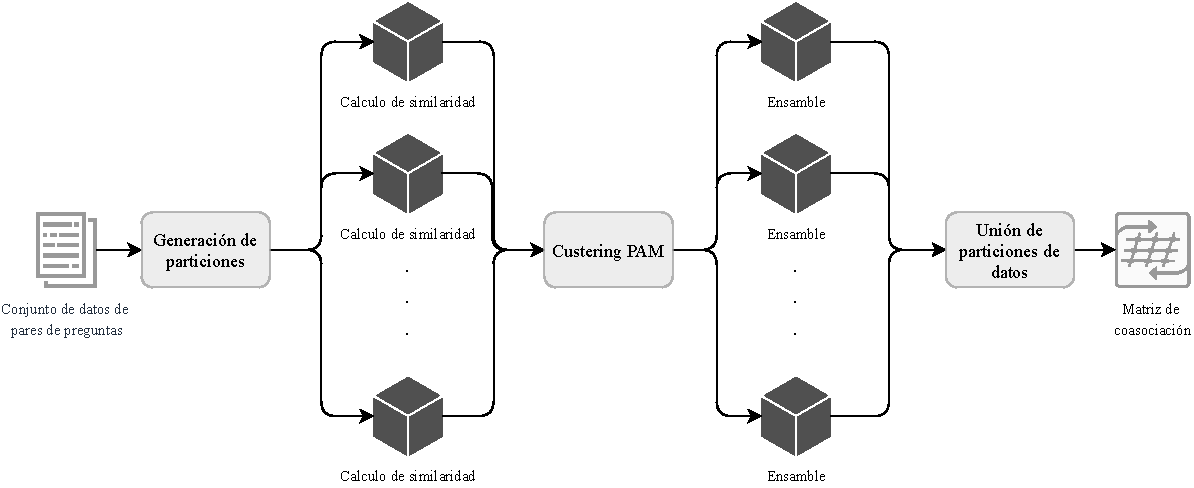
\includegraphics[width=1\linewidth]{8_problema_investigacion/imagenes/equal_distribuido}
	\caption{Infraestructura de la solución para generar una matriz de coasociación para un RS.}
	\label{fig:equaldistribuido}
\end{figure}

\bigskip Como se mencionó anteriormente, la generación de las matrices de distancia se realizarán de forma paralela, particionando el conjunto de datos de entrada y luego juntando los resultados para construir cada una de las matrices. Una vez que las matrices de similaridad son generadas en la memoria del nodo maestro se procederá a realizar el algoritmo de cluster en el mismo, paralelizando las distintas ejecuciones con el objetivo de optimizar los recursos de hardware y reducir el tiempo de ejecución. Las razones por la cual se eligió esta estrategia (en lugar de paralelizar la ejecuciones en todo el cluster de computadoras), son las siguientes:

\begin{itemize}
	\item Apache Spark no provee la funcionalidad de “replicar” un conjunto de datos y enviar tareas a un ejecutor en particular, para luego replicar el resultado. Es decir, si quisiéramos llevar a cabo el algoritmo de clustering en un nodo de datos en particular utilizando la matriz de similaridad completa y, al mismo tiempo, duplicar esta tarea tantas veces como ejecutores existan, podría optimizarse la utilización de recursos y aprovechar el paralelismo en cada uno de ellos. Por el momento, no existe una forma fácil y computacionalmente eficiente de realizar esta tarea, en una arquitectura basada en Hadoop.
	\item Evitar \textit{data-shuffling} excesivo entre entre nodos de datos. El data-shuffling es una operación que simplemente re-organiza y re-distribuye datos entre las particiones de datos apropiadas \citep{zhang2012optimizing}. Esto es un problema cuando se realiza de forma excesiva en un cluster de computadoras, provocando demasiada transferencia de datos entre cada uno de los nodos. Por ejemplo, antes de aplicar una función personalizada, en cuando se realiza shuffling puede ser necesario realizar un ordenamiento local en cada partición, re-particionar los datos en cada una de las computadoras para luego redistribuir las mismas dependiendo, por ejemplo, en una clave primaria. Dicho esto, queda en evidencia que este procedimiento conlleva un procesamiento de red y disco rígido (entrada/salida) que deriva en el incremento de tiempo de ejecución comparado con un ambiente que use una sola computadora y el intercambio de datos entre particiones se realice en la memoria local.
\end{itemize}

El algoritmo de clustering realizado en forma centralizada producirá como resultados archivos persistidos en el almacenamiento local que posibiliten aplicar un paralelismo basado en datos en el cuando el ensamble de clustering es aplicado. El formato de salida de cada una de las ejecuciones del algoritmo de clustering aplicado, posibilitarán que sea muy simple aplicar una función personalizada de ensamble de clustering distribuyendo los datos entre todas las particiones del cluster de computadoras y obteniendo una matriz de coasociación.

\subsubsection{Escalabilidad horizontal}
Es sabido que una computadora con una mejor configuración puede realizar más tareas que una con una configuración más débil, pero eso tiene una limitante. El costo de producir una computadora con buen rendimiento es alto, y no lo suficiente para justificar el costo. Por lo cual, la arquitectura elegida utiliza un cluster de computadoras para lograr un gran desempeño.

\bigskip Este tipo de sistemas escalan de una forma casi lineal con el número de servidores utilizados, y esto es posible debido al uso de particionamiento de datos \citep{pokorny2013nosql}. La distribución de datos horizontal posibilita dividir los cálculos computacionales en diferentes tareas concurrentes. Esto no es posible realizarlo fácilmente sin un algoritmo y una arquitectura que se adapte y sean pensados desde su concepción para este tipo de funcionalidad, tales como MapReduce y Hadoop.

\subsubsection{Escalabilidad y complejidad temporal}
En cuanto a la etapa de cálculo de similaridad para los distintos algoritmos tenidos en cuenta para el ensamble de clustering, siendo \(n\) el número de pares de preguntas de una muestra, y \(p = 2n\) el número de preguntas individuales. Al calcular la matriz triangular con entrada \(p\), tenemos:
\[\frac{p(p-1)}{2} = \frac{2n(2n-1)}{2} = 2n^2-n\]

Es decir, si el número de pares es \(n\), se realizarán \(2n^2-n\) cálculos por cada algoritmo de similaridad ejecutado. Además, si, por ejemplo, utilizamos \(\theta\) algoritmos de similaridad el número de cálculos de similaridad es aproximadamente \(\theta(2n2-n)\). Esto significa que al hacer cálculos de similaridad “todos contra todos” la complejidad temporal aumenta cuadráticamente, es decir \(O(n2)\)\footnote{La notación Big-O es el lenguaje y métrica que describe la eficiencia de un algoritmo. Simboliza una cota superior sobre el tiempo, basándose en una función en la cual la variable independiente puede cambiar dependiendo de la naturaleza del algoritmo (por ejemplo, tamaño de la estructura de datos o cantidad de iteraciones). \citep{cormen2009introduction}}\footnote{La notación Big-O tiende a eliminar constantes y términos no dominantes, ya que solo se centra en indicar cómo el algoritmo escala. }. Siendo estrictos, \(\theta(2n2-n)\). no sería apropiado, ya que cada uno de los diferentes algoritmos de similaridad tiene distinta complejidad interna y el tiempo varía entre cada uno de ellos, es por eso que la métrica de complejidad opta por eliminar constantes y multiplicadores a favor de la simplicidad.

\bigskip Al terminar el cálculo de similaridad, la arquitectura prevista procede a realizar un algoritmo de clustering con los resultados. Otra vez, siendo \(n\) el número de ítems (preguntas individuales), \(k\) el número de clusters elegido e \(i\) el número de iteraciones, para un tiempo \(t\) para calcular la distancia entre dos preguntas, tenemos una complejidad de \(O(n \cdot k \cdot i \cdot t)\), suponiendo que todas las iteraciones son realizadas y dejando de lado la etapa de optimización de medoides para el algoritmo PAM. Por otro lado, la arquitectura propone que el cálculo de distancia se ha realizado en una etapa anterior y las mismas son almacenadas en una estructura de datos en forma de \textit{tabla hash}\footnote{Una tabla hash es una estructura de datos que asocia claves con valores. La operación principal que soporta de manera eficiente es la búsqueda mediante una función hash.} en la cual es posible obtener la distancias de dos elementos haciendo una búsqueda indexada mediante una función hash precalculada, por lo cual, la complejidad temporal promedio en un escenario ideal será de \(O(1)\) (constante), y la complejidad final de la etapa de clustering de \(O(n \cdot k \cdot i)\), y para \(N\) ejecuciones, obtendremos \(O(N \cdot n \cdot k \cdot i)\).

\bigskip Por último, la etapa de ensamble de clustering utiliza la combinación de las \(n\) preguntas individuales en las \(N\) ejecuciones del algoritmo de clustering, obteniendo \(x = N \times n\) registros. Cada uno de esos registros son agrupados mediante una función \textit{group by}, una función que tiene una complejidad conocida de  \(O(x \cdot \log(x))\). El conjunto de datos generado es combinado con sí mismo para obtener las intersecciones, es decir \(O(x^2)\). Dado que el término \(x^2\) escala más rápido que el término \(x \cdot \log(x\)) es posible simplificar la complejidad temporal a solo \(O(x^2)\), o también \(O(N^2 \cdot n^2)\).

\bigskip De forma simplificada, la complejidad total que ofrece el método propuesto es de \(O(n^2 + Nnki + N^2n^2)\), lo cual es una función cuadrática que depende de la cantidad de preguntas individuales \(n\). Lo anterior, deja en evidencia la importancia de utilizar sistemas distribuidos y paralelismo basado en datos, ya que si bien la cantidad de cálculos total no cambia, seria posible hacer que el valor de \(n\) (y por lo tanto la cantidad de cálculos) que trabaja cada nodo de ejecución y cada ejecutor en cada uno de ellos sea más pequeño, según la cantidad de nodos o servidores de ejecución. En un contexto ideal y como modelo simplificado, por ejemplo, si se cuenta con un cluster de computadoras de \(8\) nodos y cada uno de ellos procesa \(n/8\) (\(n_{nuevo}=n / n\acute{u}mero\_de\_nodos\)) preguntas individuales, se realizarán \((n/8)^2=n^2/64\) cálculos de similaridad en cada uno de ellos, es decir, la cantidad de cálculos total, también se reducen de forma cuadrática. El ejemplo de la Figura \ref{fig:complejidad_temporal_figura}, es el modelo simplificado anteriormente mencionado, con fines didácticos que posee paralelismo de datos perfecto, cada uno de los nodos con la misma configuración y sin tener en cuenta tiempos de entrada/salida y re-particionamiento de datos. Se muestra la curva temporal de 4 clusters distintos de computadoras, con 1, 2, 4 y 8 nodos.

\begin{figure}[h!]
	\centering
	\begin{tikzpicture}
		\centering
		\begin{axis}[
			axis lines = left,
			xlabel = $n$,
			ylabel = {$t = O(n)$},
			]
			\addplot [domain=0:10, samples=100, color=red,] {x^2};
			\addlegendentry{1 nodo}

			\addplot [domain=0:10, samples=100, color=blue,]{x^2/4};
			\addlegendentry{2 nodos}

			\addplot [domain=0:10, samples=100, color=green,]{x^2/16};
			\addlegendentry{4 nodos}

			\addplot [domain=0:10, samples=100, color=purple,]{x^2/64};
			\addlegendentry{8 nodos}
		\end{axis}
	\end{tikzpicture}
	\caption{Aproximación de funciones de complejidad temporal según la cantidad de nodos del cluster de computadoras.}
	\label{fig:complejidad_temporal_figura}
\end{figure}

\bigskip La unidad básica de Apache Spark es llamada0 tarea, y la cantidad de tareas depende del número de particiones del conjunto de datos de entrada. Cada una de las tareas se encuentra en un hilo de ejecución de una JVM\footnote{Del inglés \textit{Java Virtual Machine}, es una máquina virtual que permite ejecutar programas en código intermedio Java.}, dedicado exclusivamente a un \textit{ejecutor}. Uno o más ejecutores son desplegados en los distintos \textit{nodos} del cluster de computadoras \citep{janardhanan2020optimum}. Es decir, que el paralelismo obtenido por la infraestructura Spark, depende de los tres niveles: tareas, ejecutores y nodos; así como también de la naturaleza del algoritmo que se ejecuta en la misma. Con el fin de dar un ejemplo aplicable al cálculo de similaridad, se configura un cluster de computadoras de 4 nodos, y 4 ejecutores en cada uno de ellos. Si cada uno de los ejecutores asigna 1-14 núcleos de CPU de forma dinámica, el número total de núcleos variará entre 4 y 56. Esto significa, que habrá de 4 a 56 tareas ejecutándose paralelamente en la infraestructura definida.

\subsection{Implementación en un sistema de recomendación de tiempo real}

Como punto de partida a esta sección, se aclara que este trabajo de tesis no cubre la implementación del RS propiamente dicho. No obstante, persigue como objetivo el desarrollo de un nuevo método para implementar la matriz de distancias asociada al RS, a partir de un gran volumen de datos de entrada, en particular en CQA, y utilizando una arquitectura Big Data. Para tal fin, se propondrá un ejemplo de RS a tiempo real, que dará contexto al trabajo en cuestión. El ejemplo será desarrollado teniendo en cuenta 3 casos de uso diferentes: \begin{enumerate*} [label=(\roman*)] \item un proceso batch ejecutado periódicamente que actualizará la base de datos, caso de uso central de este trabajo y en el cual se sustenta toda la arquitectura propuesta, y que también puede pensarse como una parte integrante de la implementación propuesta en este apartado; \item el punto de vista del usuario que consulta una pregunta en el sitio y \item el caso en que el usuario agrega una nueva pregunta al sitio.\end{enumerate*}

\subparagraph{El proceso completo del sistema de recomendación}
Un sistema de recomendación completo se puede analizar teniendo en cuenta 3 casos de uso, uno de los cuales es el planteado en esta Tesis.
\bigskip El primer caso de uso consiste en un proceso que se ejecuta fuera de línea, el mismo es el encargado de actualizar las relaciones de similaridad entre todas las preguntas existentes en el sitio, utilizando el método EQuAL para perseguir tal fin, y utilizando la arquitectura Big data planteada. Este es el caso analizado en esta Tesis. El segundo caso de uso consiste en la consulta de una pregunta en el sitio. Este caso se nutre del caso de uso anterior, y utiliza sus resultados para obtener una lista de preguntas similares a la consultada. Por último, si bien el procesamiento batch tiene en cuenta todas las preguntas existentes, no posee la capacidad de recomendar preguntas similares, en tiempo real, a una pregunta recién agregada al sistema. Por lo anterior, el tercer caso de uso se trata de una actualización, en la que un usuario agrega una nueva pregunta al sitio, y la resolución como implementación tecnológica para nutrir la base de datos original con nuevas preguntas y relaciones entre las mismas, en tiempo real.

\bigskip Se dará una propuesta de implementación de un RS completo, para dar contexto y tener una idea de funcionamiento en conjunto del mismo. En el mismo, se incluye como parte componente el método propuesto en esta Tesis y su arquitectura subyacente.

\subsubsection{Arquitectura general}
La arquitectura del RS embebido en un sitio de CQA colaborativo, consiste básicamente de un microservicio dedicado a recomendación, un proceso de \textit{streaming}\footnote{En computación, un \textit{stream} (en español, \textit{flujo}) es una secuencia de elementos de datos disponibles durante un periodo de tiempo.} que realizará la función de recomendación a tiempo real de forma distribuida utilizando el método EQuAL, una base de datos altamente escalable NoSQL, y un proceso batch que generará una actualización de la misma de forma periódica.

\begin{figure}
	\centering
	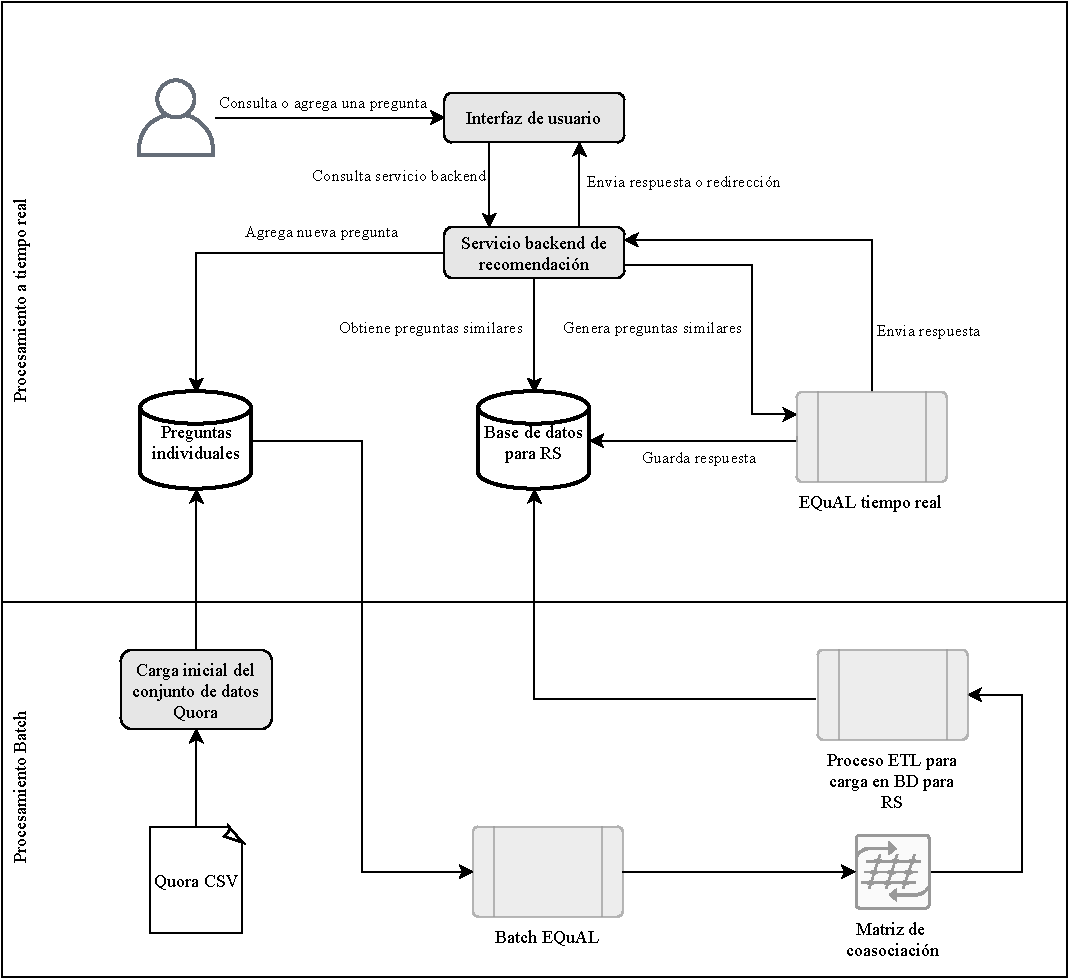
\includegraphics[width=0.9\linewidth]{8_problema_investigacion/imagenes/implementacion_rs}
	\caption{Arquitectura de un sistema de recomendación a tiempo real utilizando el método EQuAL.}
	\label{fig:implementacionrs}
\end{figure}

La Figura \ref{fig:implementacionrs} muestra cómo interactúa la totalidad de componentes relativos al RS, divididos fundamentalmente en procesamiento a tiempo real y batch; y además, muestra todas las interacciones posibles entre los componentes. Más adelante, se explicaran cada uno de los 3 casos de uso más importantes e identificables dentro de este sistema.

\subsubsection{Procesamiento batch}
La Figura \ref{fig:implementacionrsbatch} muestra el procesamiento batch para actualización y carga inicial de la base de datos que contendrá la matriz de coasociación en un formato adecuado para consulta, se ejecuta periódicamente pero con una carga inicial del conjunto de datos Quora en una base de datos. A continuación se detallaran cada uno de los casos.

\begin{figure}
	\centering
	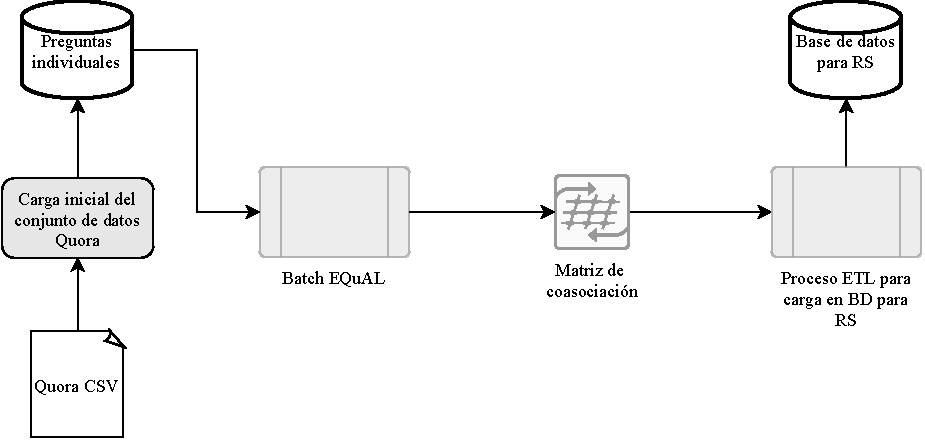
\includegraphics[width=0.9\linewidth]{8_problema_investigacion/imagenes/implementacion_rs_batch}
	\caption{Arquitectura de un sistema de recomendación a tiempo real utilizando el método EQuAL.}
	\label{fig:implementacionrsbatch}
\end{figure}

Como punto de partida y en solo una oportunidad, se carga una base de datos con el conjunto de datos Quora original. Esta base de datos podría ser relacional, o de otro tipo, pero debería tener dos características principales: rápida inserción de registros y debe permitir obtener todos los registros de una tabla mediante una sola consulta. La inserción rápida es importante en el caso del agregado de una nueva pregunta en tiempo real. La capacidad de seleccionar todos los registros de una tabla, tiene importancia para el proceso batch que utilizara el método EQuAL para la actualización periódica del RS.

\bigskip De forma periódica, proceso batch en el cual se basa este trabajo, obtendrá todas las preguntas de la base de datos de preguntas individuales para crear la matriz de coasociación. La periodicidad podrá variar dependiendo del número de clusters elegidos para el método de clustering y la arquitectura en la cual se ejecuta, mientras más rápido sea, más frecuente podría ser programado. Podría ejecutarse diariamente, en momentos de bajo tráfico en el sitio en cuestión.

\bigskip Se agrega un proceso ETL\footnote{Siglas para Extract, Transform and Load «extraer, transformar y cargar».} que tendrá como origen la matriz de coasociación y lo cargará en la base de datos que guardará la información de similaridad entre preguntas.  Las características que debe tener esta base de datos será descrita en el apartado siguiente, pero la clave principal debe ser el ID de una pregunta individual para poder ser consultada fácilmente. El proceso ETL podrá ser lanzado mediante un evento que indique que la nueva matriz de coasociación ha sido generada, o bien podría ser una extensión del proceso EQuAL. Un ejemplo de la entrada y salida de este procesamiento puede ser el que se muestra en la \textbf{Tabla \ref{tab:table-co-asociation}}. Luego del proceso ETL, los registros de la base de datos para el RS podrían tener la estructura que se muestra en la \textbf{Tabla \ref{tab:table-similar-questions}}.

\begin{table}[]
	\centering
	\begin{tabular}{|c|c|c|c|c|}
		\hline
		\textbf{question\_id\_1} & \textbf{question\_id\_2} & \textbf{question\_1} & \textbf{question\_2} & \textbf{similarity} \\ \hline
		1 & 2 & question\_desc\_1 & question\_desc\_2 & 0.34 \\ \hline
		1 & 3 & question\_desc\_1 & question\_desc\_3 & 0.67 \\ \hline
		1 & 4 & question\_desc\_1 & question\_desc\_4 & 0.92 \\ \hline
	\end{tabular}
	\caption{Matriz de coasociación salida del proceso EQuAL.}
	\label{tab:table-co-asociation}
\end{table}

\begin{table}[]
	\centering
	\begin{tabular}{|c|l|}
		\hline
		\textbf{question\_id} &
		\multicolumn{1}{c|}{\textbf{similar\_questions}} \\ \hline
		1 & \begin{lstlisting}[language=json]
[
	{
		"id": "question_id_4",
		"question": "question_desc_4",
		"similarity": "0.92"
	},
	{
		"id": "question_id_3",
		"question": "question_desc_3",
		"similarity": "0.67"
	},
	{
		"id": "question_id_2",
		"question": "question_desc_2",
		"similarity": "0.34"
	}
]
		\end{lstlisting} \\ \hline
	\end{tabular}
	\caption{Ejemplo de un registro de la base de datos de similaridad entre preguntas.}
	\label{tab:table-similar-questions}
\end{table}

Esto permitirá consultar la pregunta mediante su ID de manera muy eficiente y veloz. Por otro lado, la carga de la tabla también será muy eficiente, y que la cantidad de registros será igual a la cantidad de preguntas individuales, en lugar de la cantidad de registros de la matriz de coasociación. La columna “similar\_questions” será en formato JSON, la cual permite cargar datos con una estructura definida, y la posibilidad de serializar y deserializar los mismos de una forma estándar.

\subsubsection{Consulta de una pregunta existente}
Para este apartado, se supone que la base de datos posee toda la información necesaria y está disponible, una aplicación web que consulta un servicio backend dedicado al sistema de recomendación mediante una API REST\footnote{Representational State Transfer. Es una arquitectura y conjuntos de convenciones basada en servicios web para intercambios de información.}. Este último consultará la base de datos para devolver las preguntas similares a un ID de pregunta dado.

\begin{figure}
	\centering
	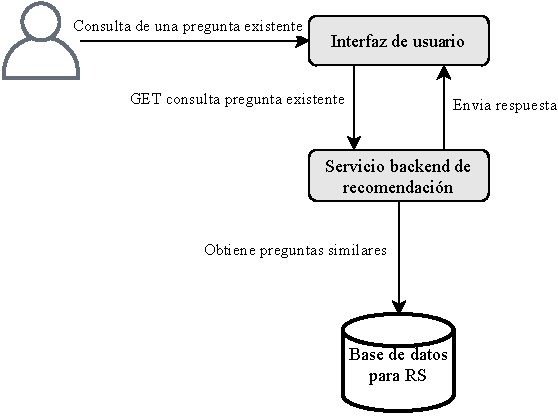
\includegraphics[width=0.6\linewidth]{8_problema_investigacion/imagenes/implementacion_rs_consulta}
	\caption{Flujo de consulta de una pregunta existente.}
	\label{fig:implementacionrsconsulta}
\end{figure}

\bigskip La Figura \ref{fig:implementacionrsconsulta} muestra el flujo de la consulta de una pregunta existente. En el momento que un usuario consulta una pregunta existente en el sitio, el servicio frontend enviará una solicitud GET al servicio backend, con el ID de la pregunta en cuestión. Este último buscará la pregunta en la base de datos utilizando el ID de pregunta y retornando todas las preguntas similares ordenadas por el valor de similaridad en forma decreciente. Esta operación debería ser ejecutada de manera rápida y eficiente, debido a un servicio backend dedicado y a una base de datos con las siguientes características:
\begin{enumerate}
	\item Una tabla con una clave primaria simple (PK), formada solo por el ID de pregunta. Esta estructura genera un índice por ID de pregunta, lo cual posibilita una búsqueda rápida.
	\item Utilizando bases de datos como Apache Cassandra,  la tabla podría estar particionada por la PK. Esto significa que se generan particiones de datos a lo largo de los diferentes nodos en el esquema de base de datos, basado en una función hash consistente y generada por el ID de pregunta. Esto es especial para búsquedas rápidas por PK.
	\item Escalabilidad.
	\item La información de preguntas similares para un ID dado, estará en formato JSON, haciendo que el servicio backend tenga un trabajo casi nulo para devolver la respuesta al frontend (una de las tareas puede ser que éste genere las URLs de las preguntas mediante los IDs).
	\item Las bases de datos como Cassandra posibilitan replicación de los registros en distintos nodos de un cluster, garantizando alta disponibilidad.
\end{enumerate}

\subsubsection{Agregar una nueva pregunta}
Agregar un nuevo item a un RS puede ser uno de los desafíos más grandes para los arquitectos de software. El propósito principal es el cálculo en tiempo real de los ítems recomendados para el ítem recién agregado al sistema, y que esto no signifique una sobrecarga del mismo. La arquitectura propuesta a continuación, que se detalla en la Figura \ref{fig:implementacionrsagregar}, intenta que las preguntas similares estén disponibles, para una pregunta nueva recién agregada, con el fin de que el usuario que realiza una pregunta en el sitio, pueda ser recomendado con otras y, también, para que cualquier otro usuario pueda tener esa información disponible tan pronto como sea posible.

\begin{figure}
	\centering
	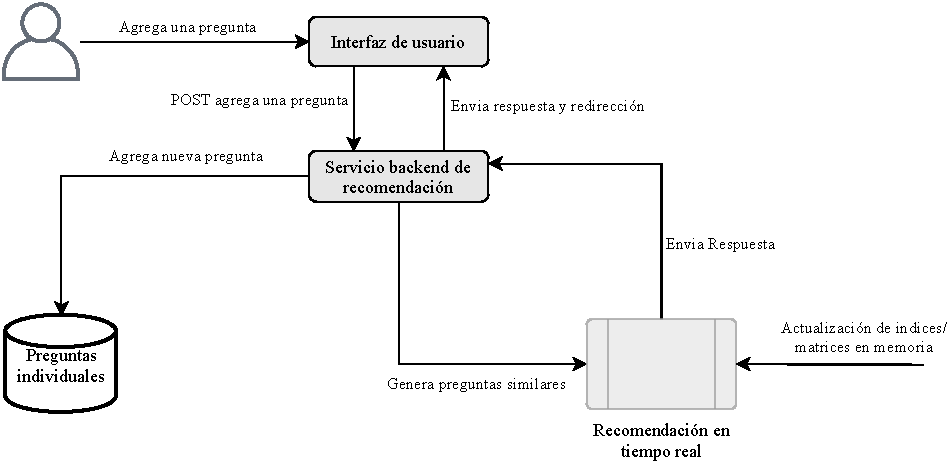
\includegraphics[width=0.9\linewidth]{8_problema_investigacion/imagenes/implementacion_rs_agregar}
	\caption{Flujo en el RS a tiempo real cuando se agrega una nueva pregunta al sistema.}
	\label{fig:implementacionrsagregar}
\end{figure}

\subsubsection{Condiciones institucionales para el desarrollo de la tesis. Infraestructura y equipamiento}
El presente trabajo se lleva a cabo en el marco del Proyecto PID UTN: Minería de Datos aplicado a problemáticas de Big Data de la Universidad Tecnológica Nacional, Facultad Regional Rosario\footnote{Código del PID: SIUTNRO0005006. Bajo la dirección del Ing. Eduardo Amar.}.

\bigskip El candidato cursó la Maestría en Ingeniería en Sistemas de Información en dicha Facultad y tendrá a disposición el equipamiento e instalaciones del Departamento en Ingeniería en Sistemas de Información. Con el objetivo de realizar el desarrollo tecnológico de este trabajo de tesis, el candidato utilizará equipos propios así como también los equipos de la universidad, en caso de que sea necesario. Los conjuntos de datos para la experimentación y validación de la solución propuesta están disponibles libremente en Internet, así como también el software y herramientas necesarias.





















	\chapter*{Capitulo 5}\label{ch:experimentos}
\addcontentsline{toc}{chapter}{Capitulo 5. Experimentos}

\section{Experimentos}
\subsection{Estado del arte}
El proyecto en el cual se realizaron los experimentos que este trabajo tiene como estado del arte, es un proyecto basado en código Python que se puede encontrar en el siguiente repositorio GitHub \url{https://github.com/Departamento-Sistemas-UTNFRRO/text_comparison}.

\bigskip Tiene como características principales la utilización de los 5 algoritmos de similaridad mencionados anteriormente (y evaluados a continuación) y la ejecución de cada uno de ellos en el marco de un patrón master-worker en un solo microprocesador. Este patrón es utilizado para el procesamiento paralelo, en el cual una tarea es enviada a cada uno de los “workers” para ser procesada. En este caso en particular, la cantidad de “workers” es fija y especificada como un parámetro en tiempo de ejecución.

\subsubsection{Análisis de rendimiento}
Se muestra al análisis de rendimiento para el cálculo de distancias con los el proyecto del estado del arte, con el fin de tener un punto comparativo para los experimentos que se realizarán con la nueva arquitectura. Las pruebas de los algoritmos de similaridad de rendimiento se realizaron con el siguiente equipo:

\begin{verbatim}
Modelo: MacBook Pro
Procesador: Intel Core i7
Velocidad del procesador: 2.6 GHz
Numero de nucleos: 6
Caché L2 (por núcleo): 256 KB
Caché L3: 12 MB
Tecnología Hyper-Threading: Habilitada
Memoria: 16 GB RAM
Almacenamiento: APPLE SSD AP0512M
\end{verbatim}

El cual también será utilizado para las pruebas de la nueva arquitectura. Se utilizará, como parámetro de rendimiento, el cálculo de similaridad para cada uno de los 404290 pares de preguntas. Luego de varias pruebas, se llega a una configuración de 8 hilos de ejecución y lotes de 10000 pares de preguntas, para obtener los tiempos más bajos posibles con cada uno de los algoritmos, los mismos fueron:

\subparagraph{Bag of Words}
\begin{verbatim}
[13:34:51] Starting script.
[13:34:51] Loading Quora questions file...
[13:34:52] ----- Run number 1 ------
[13:34:56] First 100000 distances calculated.
[13:34:58] First 200000 distances calculated.
[13:35:01] First 300000 distances calculated.
[13:35:03] First 400000 distances calculated.
[13:35:04] First 404290 distances calculated.
[13:35:04] Script finished. Total time: 0:00:12.895492
\end{verbatim}

\subparagraph{TF/IDF}
\begin{verbatim}
[13:31:05] Starting script.
[13:31:05] Loading Quora questions file...
[13:31:07] ----- Run number 1 ------
[13:31:07] Generating a sample of 0 questions.
[13:31:08] Training model...
[13:32:43] First 100000 distances calculated.
[13:33:20] First 200000 distances calculated.
[13:33:58] First 300000 distances calculated.
[13:34:38] First 400000 distances calculated.
[13:34:39] First 404290 distances calculated.
[13:34:39] Script finished. Total time: 0:03:33.665420
\end{verbatim}

\subparagraph{FastText}
\begin{verbatim}
[13:39:25] Starting script.
[13:39:25] Loading Quora questions file...
[13:39:26] ----- Run number 1 ------
[13:39:28] Training model...
Read 9M words
Number of words:  30823
Number of labels: 0
Progress: 100.0% words/sec/thread:  147553 lr:  0.000000 loss:  1.791601 ETA:   0h 0m
[13:40:29] First 100000 distances calculated.
[13:40:47] First 200000 distances calculated.
[13:41:06] First 300000 distances calculated.
[13:41:24] First 400000 distances calculated.
[13:41:25] First 404290 distances calculated.
[13:41:25] Script finished. Total time: 0:02:00.335008
\end{verbatim}

\subparagraph{Word2Vec}
\begin{verbatim}
[13:42:29] Starting script.
[13:42:29] Loading Quora questions file...
[13:42:30] ----- Run number 1 ------
[13:42:34] First 100000 distances calculated.
[13:42:36] First 200000 distances calculated.
[13:42:38] First 300000 distances calculated.
[13:42:39] First 400000 distances calculated.
[13:42:40] First 404290 distances calculated.
[13:42:40] Script finished. Total time: 0:00:10.719605
\end{verbatim}

\subparagraph{Semantic Distance}
\begin{verbatim}
[16:04:34] Starting script.
[16:04:34] Loading Quora questions file...
[16:04:35] ----- Run number 1 ------
[16:26:11] First 100000 distances calculated.
[16:47:20] First 200000 distances calculated.
[17:08:41] First 300000 distances calculated.
[17:30:08] First 400000 distances calculated.
[17:31:06] First 404290 distances calculated.
[17:31:06] Script finished. Total time: 1:26:32.941992
\end{verbatim}

\begin{table}[]
	\centering
	\begin{tabular}{|c|c|c|}
		\hline
		& \textbf{Tiempo total (segundos)} & \textbf{Velocidad aproximada (calc/seg)} \\ \hline
		\textbf{Bag of words} & 12.895492 & 31351.26601 \\ \hline
		\textbf{TF/IDF} & 213.66542 & 1892.163926 \\ \hline
		\textbf{FastText} & 120.335008  & 3359.703936 \\ \hline
		\textbf{Word2Vec}  & 10.719605 & 37715.00909 \\ \hline
		\textbf{Semantic Distance} & 5192.941992 & 77.85374853 \\ \hline
	\end{tabular}
	\caption{Análisis de rendimiento de los algoritmos de similaridad del estado del arte.}
	\label{tab:performance-estado-del-arte}
\end{table}

Los resultados en \textbf{Tabla \ref{tab:performance-estado-del-arte}}  muestran una clara ventaja en términos de rendimiento para el algoritmo de similaridad Word2Vec, inmediatamente seguido por Bag of Words. TF/IDF y FastText, muestran un rendimiento aceptable pero, en comparación, aproximadamente diez veces más lentos que los anteriormente mencionados. El rendimiento del algoritmo de similaridad Semantic Distance, es muy bajo y representa un gran problema al momento de analizar grandes conjuntos de datos, pero puede ser necesario utilizarlo debido a sus buenas medidas de desempeño y error y su análisis de similaridad desde una perspectiva distinta.

\subsubsection{Medidas de desempeño y error}
Utilizando cada para de preguntas del conjunto de datos original, se calculó la matriz de confusión para cada uno de los algoritmos de similaridad. Como se puede ver en la \textbf{Tabla \ref{tab:desempeno-estado-del-arte}}.

\begin{table}[]
	\small
	\centering
	\begin{tabular}{|c|c|c|c|c|c|c|}
		\hline
		\multicolumn{3}{|l|}{\multirow{2}{*}{}} &
		\multicolumn{2}{c|}{\textbf{Predicho}} &
		\multirow{2}{*}{\textbf{Precisión}} &
		\multirow{2}{*}{\textbf{Error}} \\ \cline{4-5}
		\multicolumn{3}{|l|}{} &
		\textbf{0} &
		\textbf{1} &
		&
		\\ \hline
		\multirow{2}{*}{\textbf{TF}} &
		\multirow{2}{*}{\textbf{Real}} &
		\textbf{0} &
		0.4355 &
		0.1953 &
		\multirow{2}{*}{0.6776} &
		\multirow{2}{*}{0.3224} \\ \cline{3-5}
		&
		&
		\textbf{1} &
		0.1271 &
		0.2421 &
		&
		\\ \hline
		\multirow{2}{*}{\textbf{TF/IDF}} &
		\multirow{2}{*}{\textbf{Real}} &
		\textbf{0} &
		0.4477 &
		0.1831 &
		\multirow{2}{*}{0.6685} &
		\multirow{2}{*}{0.3315} \\ \cline{3-5}
		&
		&
		\textbf{1} &
		0.1484 &
		0.2208 &
		&
		\\ \hline
		\multirow{2}{*}{\textbf{Word2Vec}} &
		\multirow{2}{*}{\textbf{Real}} &
		\textbf{0} &
		0.4343 &
		0.1965 &
		\multirow{2}{*}{0.6788} &
		\multirow{2}{*}{0.3212} \\ \cline{3-5}
		&
		&
		\textbf{1} &
		0.1247 &
		0.2445 &
		&
		\\ \hline
		\multirow{2}{*}{\textbf{FastText}} &
		\multirow{2}{*}{\textbf{Real}} &
		\textbf{0} &
		0.5033 &
		0.1275 &
		\multirow{2}{*}{0.6725} &
		\multirow{2}{*}{0.3275} \\ \cline{3-5}
		&
		&
		\textbf{1} &
		0.2 &
		0.1692 &
		&
		\\ \hline
		\multirow{2}{*}{\textbf{Semantic Distance}} &
		\multirow{2}{*}{\textbf{Real}} &
		\textbf{0} &
		0.4877 &
		0.1431 &
		\multirow{2}{*}{\textbf{0.6797}} &
		\multirow{2}{*}{\textbf{0.3203}} \\ \cline{3-5}
		&
		&
		\textbf{1} &
		0.1772 &
		0.192 &
		&
		\\ \hline
	\end{tabular}
	\caption{Matrices de confusión para los cinco algoritmos de medidas de similaridad.}
	\label{tab:desempeno-estado-del-arte}
\end{table}

\bigskip Los resultados porcentuales de las matrices de confusión se muestran en cada intersección de filas y columnas. Los resultados reales se muestran en las filas, siendo los dos posibles 0, cuando las preguntas son distintas y 1 cuando las preguntas son iguales. Los resultados predichos, se muestran en las columnas.
La precisión obtenida de las matrices de confusión, que se calcula como la suma de los resultados acertados entre los valores predichos y reales, en todos los casos exceden el \(66\%\), alcanzando un máximo de \(68\% \) para Word2Vec. Por otro lado, con respecto al error promedio, se llega a un valor máximo de \(33\%\) en el caso de TF/IDF.

\bigskip Observando las matrices de confusión, se presenta un desbalance en los dos valores tomados para calcular la precisión, siendo que los resultados obtenidos para la clase “0” considerablemente mejores que para la clase “1”. Por ejemplo, el desbalance más grande se encuentra en la matriz de confusión de FastText, el cual es \(0,504 – 0,170 = 0,334\). Este tipo de desbalance puede ser originado por la distribución del conjunto de datos de entrada (\(36,9\%\) pares de preguntas son clase 1 y el \(63,1\%\) restante es clase 0), el cual pretende ser corregido con un método de muestreo explicado más adelante.















\subsection{Preprocesamiento del conjunto de datos}

La calidad de un conjunto de datos del mundo real depende del número de errores que contenga. Los errores de entrada de datos, tanto simples como complejos, son muy frecuentes, más allá de las validaciones que se les hayan realizado a los mismos \citep{maletic2000data}. Además de los errores de datos, que es necesario eliminarlos, también es crucial preprocesar los mismos con el fin de estandarizar algunos factores y así obtener mejores resultados.

\bigskip Para el conjunto de datos de preguntas del sitio web Quora, se realizaron los siguientes trabajos de preprocesamiento:

\begin{enumerate}
	\item Convertir el texto en minúscula; esto habilita a que las comparaciones de texto entre preguntas con algoritmos que son sensibles al cambio entre letras mayúscula y minúscula, sean efectivas.
	\item Eliminar fórmulas; las cuales están encerradas entre etiquetas [math][/math] y [code][/code] ya que su análisis es muy complejo y contraproducente en términos de rendimiento.
	\item Reemplazar números por letras; posibilita poner en el mismo plano preguntas que contienen números y otras que no lo hacen. Además, al utilizar palabras del inglés es posible que las mismas se encuentren en taxonomías para comparaciones semánticas.
	\item Eliminar caracteres especiales, ya que los datos deben ser uniformes. Un signo de exclamación o de pregunta no cambiaría la semántica de la pregunta (desde la perspectiva del análisis de similaridad) y agregaría ruido al momento de procesarlas.
\end{enumerate}

Para resumir, cada una de las preguntas, será parámetro de una función que aplica las técnicas anteriormente mencionadas, tal como la que se muestra en el fragmento de codigo \ref{lst:funcion-limpieza}

\bigskip

\begin{python}[caption={Ejemplo de función de limpieza.}, captionpos=b,label={lst:funcion-limpieza}]
def clean_text(text):
	text = text.lower()
	text = remove_formulas(text)
	text = replace_numbers(text)
	text = remove_special_delimiters(text)

	return text
\end{python}

\bigskip Ejemplos de la salida de la función de limpieza, pueden ser:

\begin{verbatim}
i: How do I find the zeros of the polynomial function
[math]f(x)=\dfrac{1}{2}x^{3}-3x[/math]?
o: how do i find the zeros of the polynomial function
\end{verbatim}

\begin{verbatim}
i: Would you switch from Canon 6D to Leica D-LUX 109?
o: would you switch from canon six d to leica d-lux one zero nine
\end{verbatim}

En la primera, es posible ver cómo se elimina la fórmula polinómica, mientras que en la segunda, todos los números fueron transformados a letras, con espacios entre ellos. En ambas, se puede ver que el signo de interrogación se elimina y todas las letras están en minúscula.

\subsection{Muestreo del conjunto de datos}
\subsection{Generación de particiones}
\subsubsection{Cálculo de similaridades}
Se generan particiones desde los subconjuntos de muestreos generados desde el conjunto de datos original. Teniendo en cuenta que se va a utilizar un método de clustering para desarrollar el método de este trabajo, es necesario descomponer la estructura de los archivo de entrada, el cual contiene un identificador por par de preguntas, en preguntas individuales, con el fin de poder identificarlas unívocamente y poder utilizarlas como los objectos entrada del análisis de clustering. La estructura de los subconjuntos de muestreo se clarifican en la \textbf{Tabla \ref{tab:archivo-entrada}}.

\begin{table}[]
	\centering
	\begin{tabular}{|c|c|c|c|}
		\hline
		\textbf{sequence\_id} & \textbf{question\_pair\_id} & \textbf{question\_1} & \textbf{question\_2} \\ \hline
		0                     & 123004                      & question\_10         & question\_20         \\ \hline
		1                     & 98776                       & question\_11         & question\_21         \\ \hline
	\end{tabular}
	\caption{Ejemplo de la estructura de los subconjuntos de muestreo.}
	\label{tab:archivo-entrada}
\end{table}

Luego, el conjunto el subconjunto de preguntas preparado para el cálculo de distancia será generado de la siguiente forma:
\begin{enumerate}
	\item Se crea una matriz con la unión de las columnas \(question_1\) y \(question_2\), generando una fila por cada pregunta individual y un número secuencial que las identificará.
	\item Se realiza una combinación de cada una de las filas contra la matriz en sí misma (eliminando resultados repetidos), generando como resultado una estructura de matriz triangular como se muestra en la Tabla \ref{tab:matriz-triangular}.
\end{enumerate}

\begin{table}[]
	\centering
	\begin{tabular}{|c|c|c|c|}
		\hline
		\textbf{sequence\_id\_1} & \textbf{question\_id\_1} & \textbf{sequence\_id\_2} & \textbf{question\_id\_2} \\ \hline
		0 & question\_0 & 1 & question\_1 \\ \hline
		0 & question\_0 & 2 & question\_2 \\ \hline
		0 & question\_0 & 3 & question\_3 \\ \hline
		1 & question\_1 & 2 & question\_2 \\ \hline
	\end{tabular}
	\caption{Ejemplo de la estructura de matriz triangular en formato de tabla.}
	\label{tab:matriz-triangular}
\end{table}

\bigskip La estructura de matriz triangular sirve de entrada para el cálculo de similaridad por cada una de las técnicas previamente mencionadas. Por lo cual, es posible realizar un cálculo de similaridad entre las dos preguntas que pertenecen a una misma fila, y agregar esta información a la estructura de datos anterior, tal como se muestra en la Tabla \ref{tab:matriz-similaridad}.

\begin{table}[]
	\centering
	\begin{tabular}{|c|c|c|c|c|}
		\hline
		\textbf{sequence\_id\_1} & \textbf{question\_id\_1} & \textbf{sequence\_id\_2} & \textbf{question\_id\_2} & \textbf{similarity} \\ \hline
		0 & question\_0 & 1 & question\_1 & similarity\_01 \\ \hline
		0 & question\_0 & 2 & question\_2 & similarity\_02 \\ \hline
		0 & question\_0 & 3 & question\_3 & similarity\_03 \\ \hline
		1 & question\_1 & 2 & question\_2 & similarity\_12 \\ \hline
		1 & question\_1 & 3 & question\_3 & similarity\_13 \\ \hline
		2 & question\_2 & 3 & question\_3 & similarity\_23 \\ \hline
	\end{tabular}
	\caption{Ejemplo de la estructura de matriz de similaridad en formato de tabla.}
	\label{tab:matriz-similaridad}
\end{table}

\bigskip Si se piensa el subconjunto de datos anterior como en forma de matriz, en lugar de estructura de tabla, al calcular la distancia de cada una de las filas, se estaría formando una matriz triangular superior, en la cual cada uno de los elementos es la distancia entre un par de preguntas:

\[\begin{bmatrix}0 & similarity\_01 & similarity\_02 & similarity\_03 \\ 0 & 0 & similarity\_12 & similarity\_13  \\ 0 & 0  & 0 & similarity\_23  \\ 0 & 0 & 0 & 0 \end{bmatrix}\]

\bigskip La estructura de tabla, en lugar de una estructura matricial como la anterior, es utilizada por cuestiones de tecnología. Al utilizarse Python, Apache Spark y el sistema de archivos, es posible generar archivos delimitados por comas (archivos CSV) utilizando el soporte nativo que poseen las tecnologías anteriormente mencionadas. Adicionalmente, esto posibilita crear particiones de datos de manera sencilla y procesarlas de forma distribuida. Por ejemplo, si tuviésemos un archivo CSV con \(1.000.000\) (un millón) de filas y un cluster con \(8\) nodos ejecutores, cada uno procesaría \(125.000\) filas, es decir, \(1/8\) del conjunto de datos total.

\subsubsection{Clustering y etiquetado}
Una vez que las similaridades son calculadas en forma distribuida los resultados se almacenan y son colectados por el nodo maestro para realizar un etiquetado a partir de un análisis de clustering. Si bien, la implementación de un algoritmo de clustering completamente distribuido podría ser una mejora, sobre todo si se utiliza un algoritmo que requiere un gran costo computacional y es posible crear varias particiones de datos, se optó por un algoritmo relativamente simple que se ejecuta en un entorno multihilo en el nodo principal.

\bigskip El algoritmo elegido es Clustering de Partición Alrededor de Medoids (PAM) como forma de “etiquetar” cada una de las preguntas en un determinado cluster, por cada una de las ejecuciones. Se implementó de la forma que se describe a continuación.

\paragraph{Entrada y configuración inicial}
Como entrada es utilizada la matriz de similaridades que es resultado del paso anterior, y que servirán para obtener las distancias precalculadas entre cada uno de los elementos que participan en el proceso clustering. Además, en otro arreglo en memoria, el conjunto de preguntas individuales con un identificador secuencial, con el fin de facilitar el algoritmo, tal como se muestra en la \textbf{Tabla \ref{tab:preguntas-individuales}}.

\begin{table}[]
	\centering
	\begin{tabular}{|c|c|}
		\hline
		\textbf{sequence\_id} & \textbf{question} \\ \hline
		0                     & question\_0       \\ \hline
		1                     & question\_1       \\ \hline
		2                     & question\_2       \\ \hline
		3                     & question\_3       \\ \hline
	\end{tabular}
	\caption{Ejemplo de la estructura del conjunto de preguntas individuales de la muestra en curso.}
	\label{tab:preguntas-individuales}
\end{table}

\bigskip Por cada una de las corridas de clustering (parametro de configuracion) se proporcionará un \(k\) inicial, que representa al número de clusters (o medoides) que definirá el algoritmo, y en los cuales las preguntas serán distribuidas (proceso de etiquetado); y además, son identificadas con un identificador único universal (UUID\footnote{Identificador único universal \url{https://es.wikipedia.org/wiki/Identificador\_\%C3\%BAnico_universal}} por sus siglas en inglés) con el fin de poder recuperar cada uno de los resultados cuando se realice el ensamble de Clustering de cada una de estas ejecuciones.

\paragraph{Proceso de clustering}
Como se mencionó anteriormente, el algoritmo PAM tiene dos etapas, denominadas BUILD y SWAP. Por un motivos de rendimiento y simplicidad, los experimentos son realizados solo utilizando la etapa BUILD para construir cada uno de los clusters. El algoritmo realiza una cantidad de iteraciones máxima (parámetro configurable), y por cada una de ellas se realiza el proceso descrito a continuación.

\subparagraph{Generación de etiquetas}
La generación de etiquetas significa asignar un medoide a una pregunta en particular, con el objetivo del armado de clusters.
\begin{enumerate}
	\item Se busca su similaridad con cada uno de los medoides.
	\item Se asigna la pregunta al medoide (cluster) en la cual su similaridad es máxima.
	\item Se obtiene la suma de las similaridades totales por cada medoide, y se almacena en un arreglo que será utilizado en el siguiente paso.
	\item Se generan pares (ID pregunta, ID pregunta medoide) que representarán las etiquetas utilizadas por el algoritmo de ensamble.
\end{enumerate}

\subparagraph{Actualización de medoides}
Se busca actualizar los medoides con el fin de evaluar si, luego del cambio, se consiguen mejores resultados. Esto es, por cada uno de los clusters, se obtiene la similaridad de las preguntas todas contra todas, de la siguiente manera:

\begin{enumerate}
	\item Se toma una pregunta \textit{i} de la lista, y se compara la similaridad con todas las preguntas restantes del cluster.
	\item Se suman todas las similaridades calculadas.
	\item Si esta suma es mayor a la suma de las similaridades que obtuvo el medoide actual en el paso anterior, la pregunta \textit{i} pasa a ser el nuevo medoide.
	\item Se recalculan las etiquetas \((id\_pregunta, id\_pregunta\_medoide)\)
\end{enumerate}

La \textit{generación de etiquetas} y la \textit{actualización de medoides} se realiza de forma iterativa hasta que \begin{enumerate*} [label=(\roman*)] \item los medoides convergen o; \item se llega al límite máximo de iteraciones.\end{enumerate*} La convergencia de medoides significa que los medoides calculados por la iteración actual, son exactamente los mismos que la iteración anterior, lo que indica que el resultado es óptimo (dentro de los parámetros y las capacidades del algoritmo). Por otro lado, en caso de que no se haya conseguido la convergencia, el último conjunto de clusters generado el que se tomará como válido.

\paragraph{Estructura de los resultados}
Los resultados son almacenados en un archivo CSV que posee la estructura de la \textbf{Tabla \ref{tab:salida-clustering}}.
\begin{table}[]
	\centering
	\begin{tabular}{|c|c|c|}
		\hline
		\textbf{run\_id}                       & \textbf{question\_id} & \textbf{assigned\_medoid} \\ \hline
		63815467136575428551131593057064980770 & 336                   & 856                       \\ \hline
		63815467136575428551131593057064980770 & 342                   & 856                       \\ \hline
		63815467136575428551131593057064980770 & 26                    & 358                       \\ \hline
		63815467136575428551131593057064980770 & 1364                  & 437                       \\ \hline
	\end{tabular}
	\caption{Ejemplo de la estructura del resultado de la ejecución del algoritmo de clustering.}
	\label{tab:salida-clustering}
\end{table}
Cada uno de los archivos almacena un UUID único (identico en cada una de las filas, para facilitar el algoritmo de ensamble), todas las preguntas individuales del muestreo en cuestión, y el cluster a la cual pertenecen, el cual es representado por el ID de la pregunta que fue tomada como medoide para ese cluster. Se generan tantos archivos por la cantidad de ejecuciones configuradas para cada una de las técnicas de similaridad del estado del arte. Por ejemplo, si utilizamos Word2Vec, TF, TFIDF, FastText y Semántica (5 técnicas) y se configuraron 100 ejecuciones por cada una de ellas, se obtendrán 500 archivos de etiquetas; los cuales serán la única entrada del algoritmo de ensamble de clustering.






\subsection{Ensamble de clustering}
\subsection{Método de validación}\label{metodo-validacion}

\subsubsection{Generación de conjuntos estadísticamente significativos}

Para generar resultados estadísticamente significativos se ejecutó el proceso completo de modo iterativo, variando dos parámetros principales: \begin{enumerate*} [label=(\roman*)] \item el tamaño de la muestra y \item el número de clusters \(k\)\end{enumerate*}. Como experimentos para este trabajo se realizaron ejecuciones con conjuntos de datos aleatorios de 100, 500, 1000, 1500 y 2000 pares de preguntas (200, 1000, 2000, 3000 y 4000 preguntas individuales). Para cada tamaño de muestra, se realizaron 10 muestras aleatorias manteniendo un \(k\) fijo. Por ejemplo, para un número de clusters \(k = 5\) y para un tamaño de muestra 100, se realizaron 10 ejecuciones con un conjunto de datos de entrada aleatorio. Dando un total de \(5 \times 10 = 50\) matrices de co-asociación resultado, para un \(k\) fijo.

\paragraph{Elección de los tamaños de muestra}
EEn cuanto a la elección del tamaño de muestra en el apartado anterior, se tomó en cuenta que los conjuntos de datos sean lo suficientemente grandes como para generar resultados estadísticamente significativos, pero con un tamaño apropiado para la ejecución de los experimentos de forma local, en favor de la facilidad que para la depuración de los mismos. Cuando se aumenta el tamaño de la muestra en forma lineal, la cantidad de cómputos por cada uno de los algoritmos de similaridad aumentan de forma cuadrática. Como se mencionó anteriormente, Siendo \(n\) el número de pares de preguntas de una muestra, se realizarán \(2n^2-n\) cálculos. Además, si, por ejemplo, utilizamos 5 algoritmos de similaridad el número de cálculos de similaridad es de \(5(2n^2-n)\), con el agregado de que al algoritmos de clustering PAM y el ensamble de clustering también aumentan su complejidad de una forma considerable, dependiendo de nuestro número de clusters \(k\).

\paragraph{Elección del número de clusters}
La elección del número de clusters \(k\) en los experimentos realizados sigue una lógica que busca estandarizar a los mismos a lo largo de todos los tamaños de muestras, es decir, no variar el número de clusters entre ellas, con fines de comparación. Como regla general (\textit{rule of thumb} o \textit{regla del pulgar}) se considera como número ``óptimo'' de clusters un valor de alrededor de \(\sqrt{n/2}\) \citep{kodinariya2013review}, siendo \(n\) el tamaño de la muestra. Para el número de muestras elegido (200, 1000, 2000, 3000 y 4000 preguntas individuales), los valores siguiendo esta regla serían \(k = 10\), \(k = 22\), \(k = 31\), \(k = 38\), \(k =44\).

\bigskip Los valores generados por la regla del pulgar se encuentran en un rango \([10, 44]\), por lo cual, finalmente se optó por elegir los valores de \(k\) con una separación uniforme de los mismos, para facilitar su interpretación y visualización, respetando ese rango de cobertura. Los experimentos para este trabajo se realizaron con los valores \(k = 5, 10, 15, 20, 25, 30, 35, 40, 45, 50\).

\bigskip La validación de los valores de \(k\) elegidos para realizar los experimentos serán validados en conjunto mediante el rendimiento de la matriz de co-asociación. Partiendo de la base del \textit{método del codo} para la evaluación de la performance de un algoritmo de clustering, el cual evalúa el porcentaje de variabilidad (suma de cuadrados de distancias) explicada en función del número de clusters, mediante la idea de encontrar el número mínimo de clusters por el cual agregando un cluster adicional no modelaría mejor los datos. El porcentaje de variabilidad explicado por los clusters es graficado contra el número de clusters. Los primeros clusters agregaran una información considerable al modelo, pero en cierto punto la ganancia marginal caerá dramáticamente, dando un ángulo en el gráfico \citep{bholowalia2014ebk}. La Figura \ref{fig:codo} muestra un gráfico bidimensional en el cual se compara el número de clusters (en abscisas) y la suma de cuadrados de distancias (en ordenadas) como medida de variabilidad de los clusters. En este gráfico se puede ver como luego de \(k = 5\), la suma de cuadrados de distancias varía muy poco, ya que los valores esbozan una curva con valores aproximadamente constantes luego de este punto.

\begin{filecontents*}{codo.csv}
1,400
2,200
3,130
4,80
5,40
6,25
7,24
8,23
9,22
10,21
11,20
12,19
\end{filecontents*}

\begin{figure}
	\centering
	\scriptsize
	\resizebox{\textwidth}{!}{%
		\begin{tikzpicture}
			\begin{axis}[
				xlabel={Número de clusters (k)},
				ylabel={Suma de cuadrados de distancias},
				xmin=0, xmax=12,
				ymin=0, ymax=420,
				xtick={1,2,...,12},
				ytick={0,50,...,400},
				legend pos=north west,
				ymajorgrids=true,
				grid style=dashed,
				]

				\addplot table [mark=square,x index=0, y index=1, col sep=comma] {codo.csv};
				\label{codo}

				\draw [dashed] (50,0) -- (50,400);
			\end{axis}
		\end{tikzpicture}
	}
	\caption{Ejemplo de gráfico para método del codo. Valor óptimo \(k = 5\).}
	\label{fig:codo}
\end{figure}

\bigskip Con el fin de dar una aplicación más integral al método del codo, en lugar de calcularlo por cada una de las técnicas de clustering aplicadas, el mismo se aplicará utilizando la matriz de coasociación generada a partir del ensamble. Para cuantificar y evaluar el performance, se utilizarán matrices de confusión denotarán el error entre los resultados obtenidos y la clasificación proveniente del conjunto de datos original, por cada uno de los valores de k anteriormente mencionados.

\subsubsection{Estructura de las matrices de confusión}\label{estructurasconfusion}
Una matriz de confusión, es una matriz que muestra clasificaciones predichas y reales. Una matriz de confusión puede ser de tamaño \(L \times L\) donde \(L\) es el número de diferentes valores de etiqueta o clase \citep{provost1998glossary}. En este trabajo, las clases son: 0 (las preguntas comparadas no son iguales) y 1 (las preguntas son iguales). Por lo cual, la matriz de confusión que se deriva, se muestra en la Tabla \ref{tab:matriz-confusion}. Los valores “a” y “d” representan el porcentaje de veces que los valores predichos fueron iguales a los reales, es decir, los casos en que las preguntas fueron predichas, respectivamente, iguales o distintas y realmente lo eran. Por otro lado, “c” es la proporción de preguntas predichas distintas, que en realidad son iguales; y “d” la proporción de preguntas predichas iguales, pero son realmente distintas. El objetivo de un algoritmo con buen desempeño entonces, es maximizar “a” y “d” y, por lo tanto, minimizar “b” y “c”.

\bigskip
\begin{table}[h!]
	\footnotesize
	\centering
	\caption{Matriz de confusión para validación de resultados.}
	\begin{tabularx}{0.35\textwidth}{*{7}{>{\centering\arraybackslash}X}}
		\toprule
		\multicolumn{2}{l}{\multirow{2}{*}{}} & \multicolumn{2}{c}{\textbf{Predicho}}                             \\ \cmidrule(l){3-4}
		\multicolumn{2}{l}{}                  & \multicolumn{1}{c}{\textbf{0}} & \multicolumn{1}{c}{\textbf{1}} \\ \midrule
		\multicolumn{1}{c}{\multirow{2}{*}{\textbf{Real}}} & \multicolumn{1}{c}{\textbf{0}} & \multicolumn{1}{c}{a} & \multicolumn{1}{c}{b} \\ \cmidrule(l){2-4}
		\multicolumn{1}{c}{}  & \textbf{1}  & c                               & d                               \\ \bottomrule
	\end{tabularx}
	\label{tab:matriz-confusion}
\end{table}

Los indicadores de desempeño que se evaluarán en los experimentos realizados con fines comparativos, son los siguientes:
\begin{itemize}
	\item \textbf{Exactitud:} \((a+d)/(a+b+c+d)\)
	\item \textbf{Error:} \((b+c)/(a+b+c+d)\)
	\item \textbf{Precisión positivos:} \(d/(d + b)\)
	\item \textbf{Precisión negativos:} \(a/(a+c)\)
	\item \textbf{Sensitividad:} \(d/(c+d)\)
	\item \textbf{Especificidad:} \(a/(a+b)\)
\end{itemize}
donde \(a+b+c+d=1\).

\paragraph{Preparación de los datos}
Para evaluar el rendimiento del algoritmo de ensamble, se toma la matriz de coasociación generada como resultado del proceso total y la muestra de pares de preguntas que se utilizó como entrada para ese proceso. Por ejemplo, se considera la muestra de preguntas de la Tabla \ref{tab:muestra-validacion}, la cual muestra dos pares de preguntas (\(123004\) y \(98776\) - 4 preguntas en total) con su identificador de par y un indicador, en la columna \(equal\), que tiene dos valores posibles: 1 (preguntas iguales) y 0 (preguntas distintas). Por otro lado, en la Tabla \ref{tab:coasociacion-validacion}, se muestra la matriz de coasociación generada, por el método EQuAL, a partir de la Tabla \ref{tab:muestra-validacion}, teniendo en cuenta todas las combinaciones tomadas de a 2 de las 4 preguntas originales, para las cuales se agrega la similaridad entre pares, en la columna similarity. Por último, se filtran solo los pares de preguntas de la matriz de coasociación que se encuentran en la Tabla \ref{tab:muestra-validacion}, ya que son las únicas con la cual su similaridad puede compararse con fines de validación, es decir, el conjunto de datos mostrado en la Tabla \ref{tab:filtrado-validacion}. Lo que nos deja con un conjunto de pares de preguntas que es posible comparar en su totalidad con la muestra original.

\begin{table}[h!]
	\footnotesize
	\centering
	\caption{Muestras de pares de preguntas que se utilizó como entrada del método EQuAL.}
	\begin{tabularx}{0.8\textwidth}{*{7}{>{\centering\arraybackslash}c}}
		\toprule
		\textbf{sequence\_id} & \textbf{question\_pair\_id} & \textbf{question\_1} & \textbf{question\_2} & \textbf{equal} \\
		\midrule
		0                     & 123004                      & question\_10         & question\_20         & 1              \\
		1                     & 98776                       & question\_11         & question\_21         & 0              \\
		\bottomrule
	\end{tabularx}
	\label{tab:muestra-validacion}
\end{table}

\begin{table}[h!]
	\footnotesize
	\caption{Matriz de co-asociación generada a partir de la muestra de la Tabla \ref{tab:muestra-validacion}.}
	\begin{tabularx}{\textwidth}{*{7}{>{\centering\arraybackslash}X}}
		\toprule
		\textbf{question\_id\_1} & \textbf{question\_id\_2} & \textbf{question\_1} & \textbf{question\_2} & \textbf{similarity} \\
		\midrule
		question\_10 & question\_11 & contenido & contenido & 0.857 \\
		question\_10 & question\_20 & contenido & contenido & 0.210 \\
		question\_10 & question\_21 & contenido & contenido & 0.126 \\
		question\_11 & question\_20 & contenido & contenido & 0.006 \\
		question\_11 & question\_21 & contenido & contenido & 0.368 \\
		question\_20 & question\_21 & contenido & contenido & 0.146 \\
		\bottomrule
	\end{tabularx}
	\label{tab:coasociacion-validacion}
\end{table}

\begin{table}[h!]
	\footnotesize
	\caption{Filtrado de la Tabla \ref{tab:coasociacion-validacion} con los pares de preguntas que se encuentran en la Tabla \ref{tab:muestra-validacion}.}
	\begin{tabularx}{\textwidth}{*{7}{>{\centering\arraybackslash}X}}
		\toprule
		\textbf{question\_id\_1} & \textbf{question\_id\_2} & \textbf{question\_1} & \textbf{question\_2} & \textbf{similarity} \\
		\midrule
		question\_10             & question\_11             & contenido            & contenido            & 0.857               \\
		question\_11             & question\_21             & contenido            & contenido            & 0.368               \\
		\bottomrule
	\end{tabularx}
	\label{tab:filtrado-validacion}
\end{table}

Ya se realizaron los cálculos de similaridad, los algoritmos de clustering y la matriz de co-asociación. En la siguiente sección, se procederá a interpretar los resultados obtenidos.

\paragraph{Construcción y elección del umbral correcto}
La problemática que se intenta resolver teniendo en cuenta todas las similaridades obtenidas a partir del ensamble de clustering es ¿Cuando consideramos a esas preguntas iguales y cuando no? La respuesta es simple, cuando la similaridad \(S\) entre un par de preguntas (\(q_1,q_2)\) es igual o superior a cierto umbral \(t\) se considera que son iguales (1) y distintas si sucede lo contrario (0), clarificando:
\[f(x) = \left\{ \begin{array}{lcc} 1 & si & S(q_1, q_2)\geq t
	\\ 0 & si & S(q_1, q_2) < t
\end{array} \right.\]

La elección del mejor umbral, se realiza eligiendo valores en el intervalo \((0,1)\) y evaluando cual de ellos conlleva a un mejor desempeño, es decir, que los valores calculados a partir del umbral coincidan, en una mayor medida, con el valor real proveniente de la muestra de datos. Por ejemplo, tomando valores con intervalos \(0.05\) formando un arreglo como \([0.05, 0.1, 0.15, ..., 0.90, 0.95]\), por cada uno de ellos:
\begin{enumerate}
	\item Se iteran todos los pares de preguntas.
	\item Por cada uno de los valores de similaridad, se asigna \(1\) si son mayores o iguales al umbral, \(0\) si pasa lo contrario.
	\item Si los valores asignados en el paso anterior coinciden con el valor real, se asigna un valor \textit{true} (verdadero), si no coinciden, se asigna \textit{false} (falso).
	\item Se calcula la proporción de pares de preguntas asignadas con true, es decir, que el valor real coincide con el predicho, y se obtiene la \textit{exactitud} del método.
\end{enumerate}
El valor de umbral que arroje la mayor exactitud, será el utilizado para evaluar el desempeño del método, al construir la matriz de confusión.

\bigskip Volviendo al ejemplo anterior, un umbral elegido de \(0.65\) aplicado a la Tabla \ref{tab:filtrado-validacion}, arrojaría el resultado de la Tabla \ref{tab:umbral-validacion-1} (el único par de preguntas que presenta una similaridad mayor al umbral es \((question\_10, question\_11)\), por lo cual se le asigna el valor 1). La Tabla \ref{tab:umbral-validacion-1}, muestra un resultado idéntico al conjunto de entrada, es decir, a la Tabla \ref{tab:muestra-validacion}. Lo anterior significa que los pares predichos son iguales a los pares reales. En otro caso, si el umbral que tiene mejor rendimiento fuese \(0.9\), el resultado obtenido luego del cómputo hubiese sido el de la Tabla \ref{tab:umbral-validacion-2}, el cual expone una diferencia entre el valor real y el predicho del par de preguntas \((question\_10, question\_11)\). Lo anterior denota el mayor rendimiento del umbral \(0.65\) contra el umbral \(0.9\) y su importancia en la elección del valor correcto.

\bigskip

\begin{table}[h!]
	\footnotesize
	\caption{Asignación binaria de los resultados de similaridad obtenidos en la Tabla \ref{tab:filtrado-validacion}, teniendo en cuenta un umbral de \(0.65\).}
	\begin{tabularx}{\textwidth}{*{7}{>{\centering\arraybackslash}X}}
		\toprule
		\textbf{question\_id\_1} & \textbf{question\_id\_2} & \textbf{question\_1} & \textbf{question\_2} & \textbf{equal} \\
		\midrule
		question\_10             & question\_11             & contenido            & contenido            & 1              \\
		question\_11             & question\_21             & contenido            & contenido            & 0              \\
		\bottomrule
	\end{tabularx}
	\label{tab:umbral-validacion-1}
\end{table}


\begin{table}[h!]
	\footnotesize
	\caption{Asignación binaria de los resultados de similaridad obtenidos en la Tabla \ref{tab:filtrado-validacion}, teniendo en cuenta un umbral de \(0.9\).}
	\begin{tabularx}{\textwidth}{*{7}{>{\centering\arraybackslash}X}}
		\toprule
		\textbf{question\_id\_1} & \textbf{question\_id\_2} & \textbf{question\_1} & \textbf{question\_2} & \textbf{equal} \\
		\midrule
		question\_10             & question\_11             & contenido            & contenido            & 0              \\
		question\_11             & question\_21             & contenido            & contenido            & 0              \\
		\bottomrule
	\end{tabularx}
	\label{tab:umbral-validacion-2}
\end{table}

\bigskip En conclusión, el rendimiento del algoritmo se medirá comparando la variable de clase (1 o 0) del conjunto de datos de entrada, con la variable de clase construida desde la comparación de las similaridades resultados del método y un umbral apropiado. Cuanto más pares de preguntas coincidan, mejor será el rendimiento del algoritmo, el cual se podrá visualizar mediante matrices de confusión.

\paragraph{Construcción de las matrices de confusión}
Con el fin de poder ilustrar cómo se construyen las matrices de confusión a partir de la comparación de los conjuntos de datos, se utilizará el siguiente ejemplo. Supongamos que el conjunto de datos de entrada es el que se muestra en la Tabla \ref{tab:validacion-reales}, Y el resultado obtenido luego de la elección del mejor umbral, es la Tabla \ref{tab:validacion-predichos}. Por lo cual, comparando los valores de la columna “equal", obtendremos el resultado de la Tabla \ref{tab:validacion-comparacion}. Sumarizando los resultados, la matriz de confusión derivada se muestra en la Tabla \ref{tab:validacion-confusion-ejemplo}. La exactitud obtenida a partir de este conjunto de datos y la ejecución hipotética del método es \(0.75\) (y por lo tanto, el error es \(0.25\)).

\begin{table}[h!]
	\footnotesize
	\centering
	\caption{Ejemplo de conjunto de datos de entrada (reales) para validación.}
	\begin{tabularx}{0.8\textwidth}{*{7}{>{\centering\arraybackslash}c}}
		\toprule
		\textbf{sequence\_id} & \textbf{question\_pair\_id} & \textbf{question\_1} & \textbf{question\_2} & \textbf{equal} \\
		\midrule
		0 & 123004 & question\_10 & question\_20 & 1 \\
		1 & 98776  & question\_11 & question\_21 & 1 \\
		2 & 14422  & question\_12 & question\_22 & 1 \\
		3 & 12321  & question\_13 & question\_23 & 1 \\
		4 & 999    & question\_14 & question\_24 & 0 \\
		5 & 7448   & question\_15 & question\_25 & 0 \\
		6 & 69553  & question\_16 & question\_26 & 0 \\
		7 & 2447   & question\_17 & question\_27 & 1 \\
		\bottomrule
	\end{tabularx}
	\label{tab:validacion-reales}
\end{table}

\begin{table}[h!]
	\footnotesize
	\centering
	\caption{Ejemplo de conjunto de datos de predichos por el método EQuAL.}
	\begin{tabularx}{0.8\textwidth}{*{7}{>{\centering\arraybackslash}c}}
		\toprule
		\textbf{question\_id\_1} & \textbf{question\_id\_2} & \textbf{question\_1} & \textbf{question\_2} & \textbf{equal} \\
		\midrule
		question\_10 & question\_20 & contenido & contenido & 1 \\
		question\_11 & question\_21 & contenido & contenido & 1 \\
		question\_12 & question\_22 & contenido & contenido & 0 \\
		question\_13 & question\_23 & contenido & contenido & 1 \\
		question\_14 & question\_24 & contenido & contenido & 1 \\
		question\_15 & question\_25 & contenido & contenido & 0 \\
		question\_16 & question\_26 & contenido & contenido & 0 \\
		question\_17 & question\_27 & contenido & contenido & 1 \\
		\bottomrule
	\end{tabularx}
	\label{tab:validacion-predichos}
\end{table}

\begin{table}[h!]
	\footnotesize
	\centering
	\caption{Resultado de comparación de las tablas \ref{tab:validacion-reales} y \ref{tab:validacion-predichos} para validación y construcción de matrices de confusión.}
	\begin{tabularx}{0.6\textwidth}{*{7}{>{\centering\arraybackslash}c}}
		\toprule
		\textbf{sequence\_id} & \textbf{real} & \textbf{predicho} & \textbf{resultado} & \textbf{equal} \\
		\midrule
		0 & 1 & 1 & true  & 1 \\
		1 & 1 & 1 & true  & 1 \\
		2 & 1 & 0 & false & 0 \\
		3 & 1 & 1 & true  & 1 \\
		4 & 0 & 1 & false & 1 \\
		5 & 0 & 0 & true  & 0 \\
		6 & 0 & 0 & true  & 0 \\
		7 & 1 & 1 & true  & 1 \\
		\bottomrule
	\end{tabularx}
	\label{tab:validacion-comparacion}
\end{table}

\begin{table}[h!]
	\footnotesize
	\centering
	\caption{Matriz de confusión obtenida a partir de la comparación de las tablas \ref{tab:validacion-reales} y \ref{tab:validacion-predichos}.}
	\begin{tabularx}{0.35\textwidth}{*{7}{>{\centering\arraybackslash}X}}
		\toprule
		\multicolumn{2}{l}{\multirow{2}{*}{}} & \multicolumn{2}{c}{\textbf{Predicho}}                             \\ \cmidrule(l){3-4}
		\multicolumn{2}{l}{}                  & \multicolumn{1}{c}{\textbf{0}} & \multicolumn{1}{c}{\textbf{1}} \\ \midrule
		\multicolumn{1}{c}{\multirow{2}{*}{\textbf{Real}}} & \multicolumn{1}{c}{\textbf{0}} & \multicolumn{1}{c}{0.25} & \multicolumn{1}{c}{0.125} \\ \cmidrule(l){2-4}
		\multicolumn{1}{c}{}  & \textbf{1}  & 0.125                               & 0.5                               \\ \bottomrule
	\end{tabularx}
	\label{tab:validacion-confusion-ejemplo}
\end{table}

	\chapter*{Resultados}\label{ch:resultados}
\addcontentsline{toc}{chapter}{Capitulo 6. Resultados}

\section*{Resultados}
\addtocounter{section}{1}
\setcounter{subsection}{0}

\subsection{Análisis del método propuesto}

A continuación se muestran distintas ejecuciones del método EQuAL, de forma de generar resultados estadísticamente significativos, como se explicó en el apartado 5.6 (Método de validación). Se presentan tablas correspondientes a un tamaño de muestra en particular: 100, 500, 1000, 1500 y 2000 pares de preguntas; y en cada una de ellas, las filas corresponden a un número de clusters \(k\) distinto. Además, en todas las ejecuciones se realizaron 100 ejecuciones de clustering, es decir, teniendo en cuenta que se ensamblaron 5 algoritmos del estado del arte, cada una de las ejecuciones de un valor \(k\) en particular, se realizaron un total de \(500\) ejecuciones de clustering. Como método de evaluación del rendimiento de método EQuAL, se utilizan matrices de confusión. En la tabla, se muestran, por cada fila, una matriz de confusión promedio de cada una de las 10 ejecuciones para ese tamaño de muestra y número de clusters k. Como indicador de rendimiento final, se suman las columnas “\% 0/0” y “\% 1/1” para obtener la precisión, y el error es derivado de \(1 - precisi\acute{o}n\) o sumando “\% 0/1” y “\% 1/0”. Para finalizar, se resalta el mejor resultado correspondiente a un valor k para cada tamaño de muestra.

\begin{table}[]
	\centering
	\begin{tabular}{|c|c|c|c|c|c|c|}
		\hline
		\rowcolor[HTML]{CFE2F3}
		\textbf{Número de Clusters (k)} & \textbf{\% 0/0} & \textbf{\% 0/1} & \textbf{\% 1/0} & \textbf{\% 1/1} & \textbf{Precisión} & \textbf{Error} \\ \hline
		5  & 0.475 & 0.119 & 0.203 & 0.203 & 0.678 & 0.322 \\ \hline
		10 & 0.491 & 0.103 & 0.215 & 0.191 & 0.682 & 0.318 \\ \hline
		15 & 0.444 & 0.15  & 0.164 & 0.242 & 0.686 & 0.314 \\ \hline
		20 & 0.449 & 0.145 & 0.173 & 0.233 & 0.682 & 0.318 \\ \hline
		25 & 0.435 & 0.159 & 0.15  & 0.256 & 0.691 & 0.309 \\ \hline
		\rowcolor[HTML]{D9EAD3}
		30 & 0.435 & 0.159 & 0.145 & 0.261 & 0.696 & 0.304 \\ \hline
		35 & 0.444 & 0.15  & 0.157 & 0.249 & 0.693 & 0.307 \\ \hline
		40 & 0.408 & 0.186 & 0.123 & 0.283 & 0.691 & 0.309 \\ \hline
		45 & 0.459 & 0.135 & 0.176 & 0.23  & 0.689 & 0.311 \\ \hline
		50 & 0.463 & 0.131 & 0.177 & 0.229 & 0.692 & 0.308 \\ \hline
	\end{tabular}
	\caption{Matrices de confusión promedio del método EQuAL. 100 muestras de 100 pares de preguntas cada una. }
	\label{tab:analisis-100-100}
\end{table}

\begin{table}[]
	\centering
	\begin{tabular}{|c|c|c|c|c|c|c|}
		\hline
		\rowcolor[HTML]{CFE2F3}
		\textbf{Número de Clusters (k)} & \textbf{\% 0/0} & \textbf{\% 0/1} & \textbf{\% 1/0} & \textbf{\% 1/1} & \textbf{Precisión} & \textbf{Error} \\ \hline
		5  & 0.4562 & 0.1458 & 0.1908 & 0.2072 & 0.6634 & 0.3366 \\ \hline
		10 & 0.4468 & 0.1596 & 0.1658 & 0.2278 & 0.6746 & 0.3254 \\ \hline
		15 & 0.4356 & 0.1708 & 0.1542 & 0.2394 & 0.675  & 0.325  \\ \hline
		20 & 0.4316 & 0.1748 & 0.1444 & 0.2492 & 0.6808 & 0.3192 \\ \hline
		25 & 0.4306 & 0.1758 & 0.1468 & 0.2468 & 0.6774 & 0.3226 \\ \hline
		30 & 0.4322 & 0.1742 & 0.1476 & 0.246  & 0.6782 & 0.3218 \\ \hline
		35 & 0.4334 & 0.173  & 0.1458 & 0.2478 & 0.6812 & 0.3188 \\ \hline
		40 & 0.4272 & 0.1792 & 0.1378 & 0.2558 & 0.683  & 0.317  \\ \hline
		45 & 0.439  & 0.1674 & 0.1488 & 0.2448 & 0.6838 & 0.3162 \\ \hline
		\rowcolor[HTML]{D9EAD3}
		50 & 0.4378 & 0.1686 & 0.1454 & 0.2482 & 0.686  & 0.314  \\ \hline
	\end{tabular}
	\caption{Matrices de confusión promedio del método EQuAL. 100 muestras de 500 pares de preguntas cada una. }
	\label{tab:analisis-100-500}
\end{table}

\begin{table}[]
	\centering
	\begin{tabular}{|c|c|c|c|c|c|c|}
		\hline
		\rowcolor[HTML]{CFE2F3}
		\textbf{Número de Clusters (k)} & \textbf{\% 0/0} & \textbf{\% 0/1} & \textbf{\% 1/0} & \textbf{\% 1/1} & \textbf{Precisión} & \textbf{Error} \\ \hline
		5  & 0.4488 & 0.1561 & 0.1902 & 0.2049 & 0.6537 & 0.3463 \\ \hline
		10 & 0.4482 & 0.1559 & 0.1847 & 0.2112 & 0.6594 & 0.3406 \\ \hline
		15 & 0.4502 & 0.1539 & 0.188  & 0.2079 & 0.6581 & 0.3419 \\ \hline
		20 & 0.4655 & 0.1386 & 0.2007 & 0.1952 & 0.6607 & 0.3393 \\ \hline
		25 & 0.462  & 0.1421 & 0.1957 & 0.2002 & 0.6622 & 0.3378 \\ \hline
		30 & 0.461  & 0.1431 & 0.1933 & 0.2026 & 0.6636 & 0.3364 \\ \hline
		35 & 0.4608 & 0.1433 & 0.1933 & 0.2026 & 0.6634 & 0.3366 \\ \hline
		40 & 0.466  & 0.1381 & 0.2016 & 0.1943 & 0.6603 & 0.3397 \\ \hline
		45 & 0.4445 & 0.1596 & 0.1765 & 0.2194 & 0.6639 & 0.3361 \\ \hline
		\rowcolor[HTML]{D9EAD3}
		50 & 0.4521 & 0.152  & 0.1804 & 0.2155 & 0.6676 & 0.3324 \\ \hline
	\end{tabular}
	\caption{Matrices de confusión promedio del método EQuAL. 100 muestras de 1000 pares de preguntas cada una. }
	\label{tab:analisis-100-1000}
\end{table}

\begin{table}[]
	\centering
	\begin{tabular}{|c|c|c|c|c|c|c|}
		\hline
		\rowcolor[HTML]{CFE2F3}
		\textbf{Número de Clusters (k)} & \textbf{\% 0/0} & \textbf{\% 0/1} & \textbf{\% 1/0} & \textbf{\% 1/1} & \textbf{Precisión} & \textbf{Error} \\ \hline
		5  & 0.4297 & 0.1773 & 0.1713 & 0.2217 & 0.6514 & 0.3486 \\ \hline
		10 & 0.4709 & 0.136  & 0.2035 & 0.1896 & 0.6605 & 0.3395 \\ \hline
		15 & 0.4293 & 0.1777 & 0.1633 & 0.2297 & 0.659  & 0.341  \\ \hline
		20 & 0.4269 & 0.18   & 0.1624 & 0.2307 & 0.6576 & 0.3424 \\ \hline
		25 & 0.4383 & 0.1687 & 0.171  & 0.222  & 0.6603 & 0.3397 \\ \hline
		30 & 0.4509 & 0.156  & 0.1824 & 0.2107 & 0.6616 & 0.3384 \\ \hline
		35 & 0.4599 & 0.1471 & 0.1893 & 0.2037 & 0.6636 & 0.3364 \\ \hline
		40 & 0.4439 & 0.1631 & 0.1753 & 0.2177 & 0.6616 & 0.3384 \\ \hline
		45 & 0.4485 & 0.1585 & 0.1765 & 0.2165 & 0.665  & 0.335  \\ \hline
		\rowcolor[HTML]{D9EAD3}
		50 & 0.451  & 0.156  & 0.1733 & 0.2197 & 0.6707 & 0.3293 \\ \hline
	\end{tabular}
	\caption{Matrices de confusión promedio del método EQuAL. 100 muestras de 1500 pares de preguntas cada una. }
	\label{tab:analisis-100-1500}
\end{table}

\begin{table}[]
	\centering
	\begin{tabular}{|c|c|c|c|c|c|c|}
		\hline
		\rowcolor[HTML]{CFE2F3}
		\textbf{Número de Clusters (k)} & \textbf{\% 0/0} & \textbf{\% 0/1} & \textbf{\% 1/0} & \textbf{\% 1/1} & \textbf{Precisión} & \textbf{Error} \\ \hline
		5  & 0.4409 & 0.1668 & 0.1739 & 0.2184 & 0.6593 & 0.3407 \\ \hline
		10 & 0.4496 & 0.1581 & 0.1808 & 0.2115 & 0.6611 & 0.3389 \\ \hline
		15 & 0.446  & 0.1617 & 0.1737 & 0.2186 & 0.6646 & 0.3354 \\ \hline
		20 & 0.4476 & 0.1601 & 0.1774 & 0.2149 & 0.6625 & 0.3375 \\ \hline
		25 & 0.4637 & 0.144  & 0.1914 & 0.2009 & 0.6646 & 0.3354 \\ \hline
		30 & 0.431  & 0.1767 & 0.1586 & 0.2337 & 0.6647 & 0.3353 \\ \hline
		35 & 0.4451 & 0.1626 & 0.1689 & 0.2234 & 0.6685 & 0.3315 \\ \hline
		40 & 0.4569 & 0.1508 & 0.1788 & 0.2135 & 0.6704 & 0.3296 \\ \hline
		45 & 0.428  & 0.1797 & 0.152  & 0.2403 & 0.6683 & 0.3317 \\ \hline
		\rowcolor[HTML]{D9EAD3}
		50 & 0.449  & 0.1587 & 0.1719 & 0.2204 & 0.6694 & 0.3306 \\ \hline
	\end{tabular}
	\caption{Matrices de confusión promedio del método EQuAL. 100 muestras de 2000 pares de preguntas cada una. }
	\label{tab:analisis-100-2000}
\end{table}

\begin{table}[]
	\centering
	\footnotesize
	\begin{tabular}{|
			>{\columncolor[HTML]{FFE599}}c |c|c|c|c|c|c|c|}
		\hline
		\tiny\textbf{\begin{tabular}[c]{@{}c@{}}k / \\ Tam. de muestra\end{tabular}} &
		\cellcolor[HTML]{FFE599}\textbf{100} &
		\cellcolor[HTML]{FFE599}\textbf{500} &
		\cellcolor[HTML]{FFE599}\textbf{1000} &
		\cellcolor[HTML]{FFE599}\textbf{1500} &
		\cellcolor[HTML]{FFE599}\textbf{2000} &
		\cellcolor[HTML]{FFE599}\textbf{Media} &
		\cellcolor[HTML]{FFE599}\textbf{Varianza} \\ \hline
		\textbf{5}  & 0.322 & 0.3366 & 0.3463 & 0.3486 & 0.3407 & 0.33884                         & 0.000442972                                                \\ \hline
		\textbf{10} & 0.318 & 0.3254 & 0.3406 & 0.3395 & 0.3389 & 0.33248                         & \cellcolor[HTML]{D9EAD3}{\color[HTML]{333333} 0.000416228} \\ \hline
		\textbf{15} & 0.314 & 0.325  & 0.3419 & 0.341  & 0.3354 & 0.33146                         & 0.000562112                                                \\ \hline
		\textbf{20} & 0.318 & 0.3192 & 0.3393 & 0.3424 & 0.3375 & 0.33128                         & 0.000548948                                                \\ \hline
		\textbf{25} & 0.309 & 0.3226 & 0.3378 & 0.3397 & 0.3354 & 0.3289                          & 0.0006738                                                  \\ \hline
		\textbf{30} & 0.304 & 0.3218 & 0.3364 & 0.3384 & 0.3353 & 0.32718                         & 0.000843088                                                \\ \hline
		\textbf{35} & 0.307 & 0.3188 & 0.3366 & 0.3364 & 0.3315 & 0.32606                         & 0.000663592                                                \\ \hline
		\textbf{40} & 0.309 & 0.317  & 0.3397 & 0.3384 & 0.3296 & 0.32674                         & 0.000721672                                                \\ \hline
		\textbf{45} & 0.311 & 0.3162 & 0.3361 & 0.335  & 0.3317 & 0.326                           & 0.00053654                                                 \\ \hline
		\textbf{50} & 0.308 & 0.314  & 0.3324 & 0.3293 & 0.3306 & \cellcolor[HTML]{D9EAD3}0.32286 & 0.000491712                                                \\ \hline
		\textbf{Media} &
		\cellcolor[HTML]{D9EAD3}0.312 &
		0.32166 &
		0.33871 &
		0.33887 &
		0.33466 &
		\multicolumn{1}{l|}{\cellcolor[HTML]{EFEFEF}} &
		\multicolumn{1}{l|}{\cellcolor[HTML]{EFEFEF}} \\ \hline
		\textbf{Varianza} &
		0.0003 &
		0.000373684 &
		0.000129929 &
		0.000225861 &
		\cellcolor[HTML]{D9EAD3}0.000124864 &
		\multicolumn{1}{l|}{\cellcolor[HTML]{EFEFEF}} &
		\multicolumn{1}{l|}{\cellcolor[HTML]{EFEFEF}} \\ \hline
	\end{tabular}
	\caption{Error en tamaños de muestra vs. número de clusters k, con media y varianza.}
	\label{tab:analisis-error-vs-k}
\end{table}

\bigskip En forma de resumen comparativo, se van a analizar los errores cruzando cada uno de los tamaños de muestra con el número de clusters k utilizado. En la \textbf{Tabla \ref{tab:analisis-error-vs-k}}, como así también en las tablas anteriores que se utilizaron como fuentes de datos de esta última, resulta que la media total del error de todas las ejecuciones, para todos los valores de \(k\) y para todos los tamaños de muestra, es \(0.32918\). Además, con el fin de tener documentada la estabilidad del método, se calculó la varianza promedio por tamaño de muestra que resultó tener un valor \(0.0002308676\) y la varianza promedio por valor k con un valor de \(0.0005900664\). Las \textbf{Figuras \ref{fig:errores-k-tamanos-muestra} y \ref{fig:errores-tamanos-muestra-k}} muestran los resultados de la \textbf{Tabla \ref{tab:analisis-error-vs-k}} desde dos perspectivas distintas: los errores de los valores de \(k\) a lo largo de los distintos tamaños de muestra, y los errores de los tamaños de muestra a lo largo de los distintos valores de \(k\), con el fin de poder observar cómo se comporta el método EQuAL en cada perspectiva, teniendo en cuenta variabilidad y valor absoluto de los errores promedio.

\begin{figure}
	\def\svgwidth{\linewidth}
	\input{imagenes/figura2.pdf_tex}
	\caption{Errores de los valores de k en los distintos tamaños de muestra.}
	\label{fig:errores-k-tamanos-muestra}
\end{figure}

\begin{figure}
	\def\svgwidth{\linewidth}
	\input{imagenes/figura2.pdf_tex}
	\caption{Errores de los valores de k en los distintos tamaños de muestra.}
	\label{fig:errores-tamanos-muestra-k}
\end{figure}

\bigskip En la \textbf{Figura \ref{fig:errores-k-tamanos-muestra}} se puede visualizar que los valores de error no tienen una marcada proporcionalidad con el tamaño de muestra, por el contrario, se mantienen estables a lo largo de ella, pero arrojando valores más bajos en tamaños de muestra chica, lo que indicaría que la variabilidad agregada por el método de ensamble provoca buenos resultados. Si tomamos las medias por tamaño de muestra, el error promedio mínimo es \(0.312\) para el tamaño de muestra 100 y el máximo es \(0.33887\) para el tamaño de muestra 1500, lo cual es una diferencia de solo \(0.02687\) en unidades normalizadas, es decir, rango \([0, 1]\). Por otro lado, es posible ver fácilmente que los mejores resultados (errores más bajos) fueron arrojados cuando el número de cluster aumenta (esta correspondencia será confirmada en el análisis de la \textbf{Figura \ref{fig:errores-tamanos-muestra-k}}). Por ejemplo, la curva de \(k = 50\) posee el mejor error en casi todos los tamaños de muestra.

\bigskip La Figura \ref{fig:errores-tamanos-muestra-k}, se puede observar una clara tendencia decreciente a medida que se aumenta el número de clusters, para todos los tamaños de muestra. Esto también queda en evidencia cuando se calculan las medias en cada valor de \(k\), alcanzando una media mínima de error de \(0.32286\) ubicada cuando \(k = 50\) y una media máxima de \(0.33884\) cuando \(k = 5\).

\bigskip Haciendo un análisis más profundo, que se detalla más adelante, ambos gráficos sugieren que el método se comporta mejor con valores altos de \(k\), es decir, con más clusters en los cuales las preguntas pueden ser ubicadas.
\subsection{Análisis del método propuesto y algoritmos del estado del arte}

Con el fin de realizar una comparación de los resultados del método EQuAL con los algoritmos del estado del arte, se ejecutaron experimentos con la misma metodología: 10 diferentes ejecuciones con una muestra aleatoria para cada una de ellas. En las tablas \ref{tab:equal-eda-100}-\ref{tab:equal-eda-2000}, se muestran los resultados de estos algoritmos y el mejor resultado del método EQuAL para el correspondiente tamaño de muestra, este resultado es el que se va a comparar con los métodos del estado del arte. Para ellos, se generan 10 muestras aleatorias, y ellas servirán como conjunto de datos origen para cada uno de los métodos. Esto posibilita que el cálculo de similaridad y las medidas de desempeño de cada uno de los métodos, se generen con exactamente el mismo conjunto de datos, y los resultados solamente dependan del cálculo de distancia (y del algoritmo de clustering sujeto a aleatoriedad en lo medoides del método EQuAL). Se resalta con color verde el mejor resultado (error más pequeño) por cada una de ellas.

\begin{table}[h!]
	\footnotesize
	\begin{tabularx}{\textwidth}{*{8}{>{\centering\arraybackslash}X}}
		\toprule
		&
		\textbf{k} &
		\textbf{\% 0/0} &
		\textbf{\% 0/1} &
		\textbf{\% 1/0} &
		\textbf{\% 1/1} &
		\textbf{Exactitud} &
		\textbf{Error} \\
		\midrule
		\textbf{bow} &
		--- &
		0.429 &
		0.165 &
		0.131 &
		0.275 &
		\cellcolor[HTML]{D9EAD3}0.704 &
		\cellcolor[HTML]{D9EAD3}0.296 \\
		\textbf{ft}       & --- & 0.413 & 0.181 & 0.153 & 0.253 & 0.666 & 0.334 \\
		\textbf{w2v}      & --- & 0.396 & 0.198 & 0.119 & 0.287 & 0.683 & 0.317 \\
		\textbf{gtfidf}   & --- & 0.48  & 0.114 & 0.197 & 0.209 & 0.689 & 0.311 \\
		\textbf{sem}      & --- & 0.473 & 0.121 & 0.18  & 0.226 & 0.699 & 0.301 \\
		\textbf{ensamble} & 30  & 0.463 & 0.131 & 0.177 & 0.229 & 0.692 & 0.308 \\
		\bottomrule
	\end{tabularx}
	\caption{Ensamble vs. técnicas del estado del arte. Tamaño de muestra 100 pares de preguntas y 10 ejecuciones en cada una de las técnicas.}
	\label{tab:equal-eda-100}
\end{table}

\begin{table}[h!]
	\footnotesize
	\begin{tabularx}{\textwidth}{*{8}{>{\centering\arraybackslash}X}}
		\toprule
		&
		\textbf{k} &
		\textbf{\% 0/0} &
		\textbf{\% 0/1} &
		\textbf{\% 1/0} &
		\textbf{\% 1/1} &
		\textbf{Exactitud} &
		\textbf{Error} \\
		\midrule
		\textbf{bow} &
		--- &
		0.3948 &
		0.2072 &
		0.105 &
		0.293 &
		\cellcolor[HTML]{D9EAD3}0.6878 &
		\cellcolor[HTML]{D9EAD3}0.3122 \\
		\textbf{ft}       & --- & 0.4724 & 0.1296 & 0.1986 & 0.1994 & 0.6718 & 0.3282 \\
		\textbf{w2v}      & --- & 0.3758 & 0.2262 & 0.0984 & 0.2996 & 0.6754 & 0.3246 \\
		\textbf{gtfidf}   & --- & 0.4346 & 0.1674 & 0.1544 & 0.2436 & 0.6782 & 0.3218 \\
		\textbf{sem}      & --- & 0.4648 & 0.1372 & 0.1804 & 0.2176 & 0.6824 & 0.3176 \\
		\textbf{ensamble} & 50  & 0.4378 & 0.1686 & 0.1454 & 0.2482 & 0.686  & 0.314  \\
		\bottomrule
	\end{tabularx}
	\caption{Ensamble vs. técnicas del estado del arte. Tamaño de muestra 500 pares de preguntas y 10 ejecuciones en cada una de las técnicas.}
	\label{tab:equal-eda-500}
\end{table}

\begin{table}[h!]
	\footnotesize
	\begin{tabularx}{\textwidth}{*{8}{>{\centering\arraybackslash}X}}
		\toprule
		&
		\textbf{k} &
		\textbf{\% 0/0} &
		\textbf{\% 0/1} &
		\textbf{\% 1/0} &
		\textbf{\% 1/1} &
		\textbf{Exactitud} &
		\textbf{Error} \\
		\midrule
		\textbf{bow} &
		--- &
		0.386 &
		0.2189 &
		0.096 &
		0.2991 &
		\cellcolor[HTML]{D9EAD3}0.6851 &
		\cellcolor[HTML]{D9EAD3}0.3149 \\
		\textbf{ft}       & --- & 0.4322 & 0.1727 & 0.1548 & 0.2403 & 0.6725 & 0.3275 \\
		\textbf{w2v}      & --- & 0.4134 & 0.1915 & 0.1254 & 0.2697 & 0.6831 & 0.3169 \\
		\textbf{gtfidf}   & --- & 0.4161 & 0.1888 & 0.1364 & 0.2587 & 0.6748 & 0.3252 \\
		\textbf{sem}      & --- & 0.4639 & 0.141  & 0.1752 & 0.2199 & 0.6838 & 0.3162 \\
		\textbf{ensamble} & 50  & 0.4521 & 0.152  & 0.1804 & 0.2155 & 0.6676 & 0.3324 \\
		\bottomrule
	\end{tabularx}
	\caption{Ensamble vs. técnicas del estado del arte. Tamaño de muestra 1000 pares de preguntas y 10 ejecuciones en cada una de las técnicas.}
	\label{tab:equal-eda-1000}
\end{table}

\begin{table}[h!]
	\footnotesize
	\begin{tabularx}{\textwidth}{*{8}{>{\centering\arraybackslash}X}}
		\toprule
		&
		\textbf{k} &
		\textbf{\% 0/0} &
		\textbf{\% 0/1} &
		\textbf{\% 1/0} &
		\textbf{\% 1/1} &
		\textbf{Exactitud} &
		\textbf{Error} \\
		\midrule
		\textbf{bow} &
		--- &
		0.4070667 &
		0.198 &
		0.1222667 &
		0.2726667 &
		\cellcolor[HTML]{D9EAD3}0.6797333 &
		\cellcolor[HTML]{D9EAD3}0.3202667 \\
		\textbf{ft}       & --- & 0.4736666 & 0.1314       & 0.2006667 & 0.1942667 & 0.6679333 & 0.3320667 \\
		\textbf{w2v}      & --- & 0.4266       & 0.1784667 & 0.1446667 & 0.2502667 & 0.6768667 & 0.3231337 \\
		\textbf{gtfidf}   & --- & 0.4217333 & 0.1833333 & 0.1488667 & 0.2460667 & 0.6678       & 0.3322       \\
		\textbf{sem}      & --- & 0.463        & 0.1420667 & 0.1917333 & 0.2032       & 0.6662       & 0.3338       \\
		\textbf{ensamble} & 50  & 0.451        & 0.156        & 0.1733       & 0.2197       & 0.6707       & 0.3293       \\
		\bottomrule
	\end{tabularx}
	\caption{Ensamble vs. técnicas del estado del arte. Tamaño de muestra 1500 pares de preguntas y 10 ejecuciones en cada una de las técnicas.}
	\label{tab:equal-eda-1500}
\end{table}

\begin{table}[h!]
	\footnotesize
	\begin{tabularx}{\textwidth}{*{8}{>{\centering\arraybackslash}X}}
		\toprule
		&
		\textbf{k} &
		\textbf{\% 0/0} &
		\textbf{\% 0/1} &
		\textbf{\% 1/0} &
		\textbf{\% 1/1} &
		\textbf{Exactitud} &
		\textbf{Error} \\
		\midrule
		\textbf{bow} &
		--- &
		0.402 &
		0.20455 &
		0.1102 &
		0.28325 &
		\cellcolor[HTML]{D9EAD3}0.68525 &
		\cellcolor[HTML]{D9EAD3}0.31475 \\
		\textbf{ft}       & --- & 0.46865 & 0.1379  & 0.19655 & 0.1969 & 0.66555 & 0.33445 \\
		\textbf{w2v}      & --- & 0.40985 & 0.1967  & 0.12665 & 0.2668 & 0.67665 & 0.32335 \\
		\textbf{gtfidf}   & --- & 0.43255 & 0.174   & 0.15625 & 0.2372 & 0.66975 & 0.33025 \\
		\textbf{sem}      & --- & 0.4887  & 0.11785 & 0.20705 & 0.1864 & 0.6751  & 0.3249  \\
		\textbf{ensamble} & 50  & 0.449   & 0.1587  & 0.1719  & 0.2204 & 0.6694  & 0.3306  \\
		\bottomrule
	\end{tabularx}
	\caption{Ensamble vs. técnicas del estado del arte. Tamaño de muestra 2000 pares de preguntas y 10 ejecuciones en cada una de las técnicas.}
	\label{tab:equal-eda-2000}
\end{table}

\begin{table}[h!]
	\footnotesize
	\begin{tabularx}{\textwidth}{XXXXXXXX}
		\toprule
		& \textbf{100} & \textbf{500} & \textbf{1000} & \textbf{1500} & \textbf{2000} & \textbf{Media} & \textbf{Varianza} \\
		\midrule
		\textbf{bow}      & 0.296 & 0.3122 & 0.3149 & 0.3202667 & 0.31475 & \cellcolor[HTML]{D9EAD3}0.3116233 & 0.0003396                          \\
		\textbf{ft}       & 0.334 & 0.3282 & 0.3275 & 0.3320667 & 0.33445 & 0.3312433                         & \cellcolor[HTML]{D9EAD3}0.0000418 \\
		\textbf{w2v}      & 0.317 & 0.3246 & 0.3169 & 0.3231333 & 0.32335 & 0.3209967                         & 0.0000558                         \\
		\textbf{gtfidf}   & 0.311 & 0.3218 & 0.3252 & 0.3322       & 0.33025 & 0.32409                              & 0.0002815                              \\
		\textbf{sem}      & 0.301 & 0.3176 & 0.3162 & 0.3338       & 0.3249  & 0.3187                               & 0.0005872                                \\
		\textbf{ensamble} & 0.308 & 0.314  & 0.3324 & 0.3293       & 0.3306  & 0.32286                              & 0.0004917                              \\
		\bottomrule
	\end{tabularx}
	\caption{Error en los algoritmos del estado del arte vs. método EQuAL por tamaño de muestra, media y varianza.}
	\label{tab:error-arte-equal}
\end{table}

\bigskip En forma de resumen, en la Tabla \ref{tab:error-arte-equal}, se pueden ver todos los errores por cada uno de los métodos, más la media y la varianza de cada uno de ellos. Esta tabla muestra una media de error a través de las distintas muestras aleatorias para el método EQuAL y las ejecuciones de los algoritmos del estado del arte. El método EQuAL, en este caso, muestra muy buenos resultados para los tamaños de muestra más pequeños (100 y 500), pero manteniéndose en un rango aceptable en todos los tamaños de muestra. El método propuesto en el presente trabajo posee un indicador de medias de error total a lo largo de todas las muestras de \(0.32286\). Adicionalmente, analizando las varianzas de cada uno de los métodos, se observa que el método EQuAL se encuentra en el rango esperado (media \(0.000491712\)) y es muy similar a la varianza de los demás métodos. La varianza del método EQuAL se ve afectada porque los valores tomados para el análisis anterior son los correspondientes a las ejecuciones que poseen error más bajo (variando el número de clusters) para cada tamaño de muestra. Estos indicadores se pueden visualizar en la Figura \ref{fig:ensamble-vs-medidas}. Se extiende la explicación de la variabilidad del método más adelante.

\begin{filecontents*}{ensamblevsmedidas.csv}
100,0.296,0.334,0.317,0.311,0.301,0.308
500,0.3122,0.3282,0.3246,0.3218,0.3176,0.314
1000,0.3149,0.3275,0.3169,0.3252,0.3162,0.3324
1500,0.3202666667,0.3320666667,0.3231333333,0.3322,0.3338,0.3293
2000,0.31475,0.33445,0.32335,0.33025,0.3249,0.3306
\end{filecontents*}

\begin{figure}[h!]
	\centering
	\scriptsize
	\resizebox{\textwidth}{!}{%
		\begin{tikzpicture}
			\begin{axis}[
				xlabel={Tamaños de muestra},
				ylabel={Error},
				xmin=100, xmax=2000,
				ymin=0.28, ymax=0.35,
				xtick={100,500,1000,1500,2000},
				ytick={0.28,0.29,...,0.35},
				legend pos=north west,
				ymajorgrids=true,
				grid style=dashed,
				]

				\addplot+ [line width=2pt] table [mark=none,x index=0, y index=6, col sep=comma] {ensamblevsmedidas.csv};
				\label{ensamble}
				\addplot table [mark=square,x index=0, y index=1, col sep=comma] {ensamblevsmedidas.csv};
				\label{bow}
				\addplot table [mark=square,x index=0, y index=2, col sep=comma] {ensamblevsmedidas.csv};
				\label{ft}
				\addplot table [mark=square,x index=0, y index=3, col sep=comma] {ensamblevsmedidas.csv};
				\label{w2v}
				\addplot table [mark=square,x index=0, y index=4, col sep=comma] {ensamblevsmedidas.csv};
				\label{tfidf}
				\addplot table [mark=square,x index=0, y index=5, col sep=comma] {ensamblevsmedidas.csv};
				\label{sem}
			\end{axis}

			% Cuadro de leyendas.
			\node [draw,fill=white] at (rel axis cs: 0.82,0.2) {\scriptsize\shortstack[l]{
					\ref{bow} $bow$ \\
					\ref{ft} $ft$ \\
					\ref{w2v} $w2v$ \\
					\ref{tfidf} $tfidf$ \\
					\ref{sem} $sem$ \\
					\ref{ensamble} $ensamble$}};
		\end{tikzpicture}
	}
	\caption{Errores de los tamaños de muestra para el método EQuAL y los algoritmos del estado del arte.}
	\label{fig:ensamble-vs-medidas}
\end{figure}

\subsection{Otras observaciones de interés}

\subsubsection{Análisis de varianza del método propuesto}

Con el fin de analizar si el método EQuAL es apto para su aplicación en RSs y poner en perspectiva sus resultados en comparación con los algoritmos del estado del arte, se realiza un \textit{análisis de varianza} con la aplicación del \textit{método de Tukey}.

\bigskip El análisis de varianza prueba la significancia estadística de la diferencia de medias (o tendencia central) entre los diferentes métodos en análisis. El término\textit{ estadísticamente significativo} indica que rechazar la hipótesis nula no significa que el hallazgo sea importante, sino que la diferencia media es lo suficientemente grande como para que la muestra vuelva a aparecer si los experimentos son realizados nuevamente \citep{tabachnick2007experimental}. En el caso de estudio, considerando la esperanza de error como variable en análisis, la hipótesis nula sugiere que el método EQuAL es apto, eficiente y eficaz para ser utilizado en un sistema de recomendación, en comparación con métodos ampliamente utilizados y reconocidos por la comunidad. Para clarificar, la intención de este trabajo es aceptar la hipótesis nula o, aun mejor, rechazar la hipótesis nula con una medida de rendimiento que demuestre que el método EQuAL es significativamente mejor. En este apartado se usa el análisis de varianza como una herramienta para tal fin. Si los resultados son los esperados, podemos llegar a la conclusión que el método EQuAL puede ser utilizado como medio para generar matrices de similaridad aptas para un RS eficiente y eficaz, mediante pruebas estadísticamente significativas. Se realizó un análisis de varianza\footnote{El código completo del análisis de varianza se encuentra en este repositorio GitHub \url{https://github.com/fedetesone/anova_equal}.} con los datos\footnote{Conjunto de datos fuente para el análisis de varianzas: \url{https://github.com/fedetesone/anova_equal/blob/main/resultados.csv}.} utilizados para generar las tablas resumen del apartado “\ref{ss:analisismetodoestado} Análisis del método propuesto y algoritmos del estado del arte”.

\bigskip Los algoritmos del estado del arte y método EQuAL basado en el ensamble de los mismos, generaron conjuntos de datos que son utilizados como entrada para el análisis. Se denomina \(\mu_0\) a la esperanza de los errores del método EQuAL y se denominan  \(\mu_i, i = 1,..., 5\) a las esperanzas de los errores de los métodos, TF, TFIDF, FastText, Word2Vec y Semantic Distance, respectivamente. Se plantean las siguientes hipótesis:
\begin{itemize}
	\item \textbf{\(H_0\)}: \(\mu_0 - \mu_i = 0, i = 1,..., 5\)
	\item \textbf{\(H_1\)}: \(\mu_0 - \mu_i \neq  0, i = 1,..., 5\)
\end{itemize}
Por lo mencionado, se plantean estos test de hipótesis para cada variable en forma separada.

\bigskip El análisis de medias de error a continuación se realizará comparando el método EQuAL contra los métodos del estado del arte (uno a uno), para un tamaño de muestra determinado. Para tal fin, se utiliza el método de Tukey para crear intervalos de confianza para todas las diferencias de medias, en parejas. Por lo anterior, es necesario el énfasis especial es el método EQuAL realizando comparaciones específicas mediante pares, contra cada una de las técnicas del estado del arte \citep{abdi2010tukey}. Filtrando las comparaciones uno a uno en las cuales se encuentra el método EQuAL, es posible saber cómo se comporta. Si las medias de error no tienen diferencias significativas en términos estadísticos, significa que el método EQuAL es, al menos, apto para la generación de medidas de similaridad a partir del conjunto de datos en estudio, y su aplicación en RS.

\bigskip A continuación, se muestran los métodos Tukey aplicados en R para cada uno de los tamaños de muestra tenidos en cuenta en los experimentos, utilizando un nivel de confianza de \(95\% (\alpha=0.05)\).

\paragraph{Tamaño de muestra de 100 pares de preguntas}
\begin{rc}
                 diff        lwr       upr     p adj
ensemble-bow     0.008 -0.0589175 0.0749175 0.9992360
ft-ensemble      0.030 -0.0369175 0.0969175 0.7702455
gtfidf-ensemble  0.007 -0.0599175 0.0739175 0.9996012
sem-ensemble    -0.003 -0.0699175 0.0639175 0.9999940
w2v-ensemble     0.013 -0.0539175 0.0799175 0.9923331
\end{rc}

\begin{figure}[!]
	\centering
	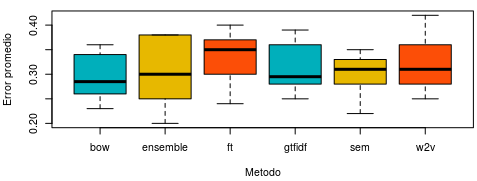
\includegraphics[width=0.7\linewidth]{10_resultados/imagenes/anova_100}
	\caption{Gráfico de caja y bigote para las medias de error de los métodos en estudio para tamaño de muestra de 100 pares de preguntas.}
	\label{fig:anova100}
\end{figure}

\bigskip El método EQuAL posee una media de error que no posee diferencias significativas a todos los métodos. En todos los casos, los intervalos de confianza incluyen al valor 0 y \(p-adj > \alpha\). La Figura \ref{fig:anova100} muestra un gráfico de caja y bigote para las medias de error en estudio y tamaño de muestra 100. En la misma, se puede visualizar que el método EQuAL posee el menor valor de error para una ejecución individual en particular, representado por el bigote inferior.

\bigskip
\paragraph{Tamaño de muestra de 500 pares de preguntas}
\begin{rc}
                  diff          lwr         upr     p adj
ensemble-bow     0.0018 -0.016671384 0.020271384 0.9997181
ft-ensemble      0.0142 -0.004271384 0.032671384 0.2237050
gtfidf-ensemble  0.0078 -0.010671384 0.026271384 0.8113536
sem-ensemble     0.0036 -0.014871384 0.022071384 0.9922183
w2v-ensemble     0.0106 -0.007871384 0.029071384 0.5407045
\end{rc}

\begin{figure}
	\centering
	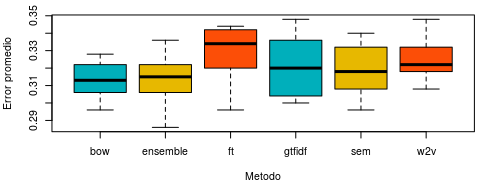
\includegraphics[width=0.7\linewidth]{10_resultados/imagenes/anova_500}
	\caption{Gráfico de caja y bigote para las medias de error de los métodos en estudio para tamaño de muestra de 500 pares de preguntas.}
	\label{fig:anova500}
\end{figure}

\bigskip El método EQuAL posee una media de error que no posee diferencias significativas a todos los métodos. En todos los casos, los intervalos de confianza incluyen al valor 0 y \(p-adj > \alpha\). La Figura \ref{fig:anova500} muestra un gráfico de caja y bigote para las medias de error en estudio y tamaño de muestra 500. En la misma, se puede visualizar que el método EQuAL posee el menor valor de error para una ejecución individual en particular, representado por el bigote inferior.

\bigskip
\paragraph{Tamaño de muestra de 1000 pares de preguntas}
\begin{rc}
                  diff          lwr         upr     p adj
ensemble-bow     0.0175 -0.004161633 0.039161633 0.1791584
ft-ensemble     -0.0049 -0.026561633 0.016761633 0.9846755
gtfidf-ensemble -0.0072 -0.028861633 0.014461633 0.9217004
sem-ensemble    -0.0162 -0.037861633 0.005461633 0.2504112
w2v-ensemble    -0.0155 -0.037161633 0.006161633 0.2956972
\end{rc}

\begin{figure}
	\centering
	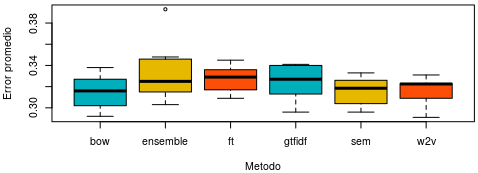
\includegraphics[width=0.7\linewidth]{10_resultados/imagenes/anova_1000}
	\caption{Gráfico de caja y bigote para las medias de error de los métodos en estudio para tamaño de muestra de 1000 pares de preguntas.}
	\label{fig:anova1000}
\end{figure}

\bigskip El método EQuAL posee una media de error que no posee diferencias significativas a todos los métodos. En todos los casos, los intervalos de confianza incluyen al valor 0 y \(p-adj > \alpha\). La Figura \ref{fig:anova1000} muestra un gráfico de caja y bigote para las medias de error en estudio y tamaño de muestra 1000.

\bigskip
\paragraph{Tamaño de muestra de 1500 pares de preguntas}
\begin{rc}
                        diff           lwr         upr     p adj
ensemble-bow     0.0090666667 -7.427521e-03 0.025560854 0.5832109
ft-ensemble      0.0027333333 -1.376085e-02 0.019227521 0.9962642
gtfidf-ensemble  0.0028666667 -1.362752e-02 0.019360854 0.9953275
sem-ensemble     0.0044666667 -1.202752e-02 0.020960854 0.9656207
w2v-ensemble    -0.0062000000 -2.269419e-02 0.010294187 0.8729702
\end{rc}

\begin{figure}
	\centering
	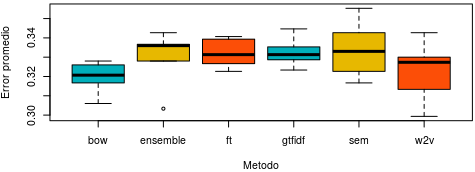
\includegraphics[width=0.7\linewidth]{10_resultados/imagenes/anova_1500}
	\caption{Gráfico de caja y bigote para las medias de error de los métodos en estudio para tamaño de muestra de 1500 pares de preguntas.}
	\label{fig:anova1500}
\end{figure}

\bigskip El método EQuAL posee una media de error que no posee diferencias significativas a todos los métodos. En todos los casos, los intervalos de confianza incluyen al valor 0 y \(p-adj > \alpha\). La Figura \ref{fig:anova1500} muestra un gráfico de caja y bigote para las medias de error en estudio y tamaño de muestra 1500.

\bigskip
\paragraph{Tamaño de muestra de 2000 pares de preguntas}
\begin{rc}
                  diff       lwr       upr      p adj
ensemble-bow     0.01585  0.001648 0.0300516 0.020523
ft-ensemble      0.00385 -0.010351 0.0180516 0.965462
gtfidf-ensemble -0.00035 -0.014551 0.0138516 0.999999
sem-ensemble    -0.00570 -0.019901 0.0085016 0.839375
w2v-ensemble    -0.00725 -0.021451 0.0069516 0.657185
\end{rc}

\begin{figure}
	\centering
	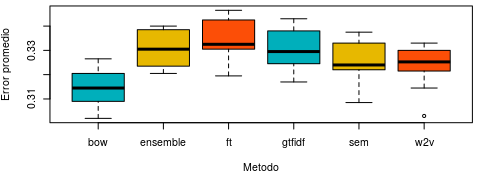
\includegraphics[width=0.7\linewidth]{10_resultados/imagenes/anova_2000}
	\caption{Gráfico de caja y bigote para las medias de error de los métodos en estudio para tamaño de muestra de 2000 pares de preguntas.}
	\label{fig:anova2000}
\end{figure}

\bigskip En este caso, el intervalos de confianza contra el método bow no incluye al cero, ya que este método tuvo muy buenos indicadores en este tamaño de muestra. No obstante, el método EQuAL tiene una diferencia significativa solo con el método bow, no habiendo diferencias significativas con los métodos restantes, ya que en esos casos, los intervalos de confianza incluyen al valor \(0\) y \(p-adj > \alpha\). La Figura \ref{fig:anova2000} muestra un gráfico de caja y bigote para las medias de error en estudio y tamaño de muestra 2000.

\bigskip
\paragraph{Resumen de resultados del análisis de varianza}
En general, el método EQuAL tiene un buen comportamiento en cuanto a medias de error a lo largo de todos los tamaños de muestra. Esto significa que las esperanzas de error no tienen diferencias significativas con los métodos del estado del arte (los cuales son utilizados por la comunidad en el cálculo de similaridad y análisis de texto) y son, incluso, superadoras en algunos casos. Teniendo en cuenta este indicador, se puede concluir que el método EQuAL es apto para su implementación en RSs.

\subsubsection{Desempeño con tamaños de muestra pequeños}
En el análisis de varianza de las medias de error realizado anteriormente, se puede observar que el método EQuAL se comporta muy bien en los tamaños de muestra de 100 y 500 pares de preguntas: el método propuesto fue estadísticamente igual o superior a los métodos del estado del arte. Sin embargo, para tamaños de muestra más grandes, fue superado en algunas oportunidades.

\bigskip Esto demuestra que el agregado de variabilidad de datos puede ser influyente en el cálculo de similaridad. Los métodos del estado del arte cada una de las preguntas de cada para entre sí, mientras que el método EQuAL realiza una comparación “todas contra todas” con el objetivo de realizar un método de clustering a continuación. Para clarificar, se puede concluir que los gráficos y estadísticas obtenidos muestran que métodos basados en ensamble de clustering, y en particular el método EQuAL,  proponen una medida de similaridad adimensional que puede mejorar ciertas medidas de rendimiento en comparativa con otros algoritmos. Citando a \cite{fred2005combining} esta mejora se hace aún más evidente en tamaños de muestras chicos o conjuntos de datos complejos.

\subsubsection{Dependencia de un método de ensamble con sus algoritmos subyacentes}
Si bien es una medida adimensional y propone mejorar las medidas de rendimiento en ciertos aspectos, los métodos de ensamble de clustering son dependientes de sus algoritmos subyacentes y, por lo tanto, las medidas de desempeño son similares en cuanto a, por ejemplo, el valor de error obtenido. Los análisis de varianza realizados ponen en evidencia la dependencia del método equal con los algoritmos ensamblados. La media de error es la misma (estadísticamente hablando) en la mayoría de los casos, lo cual indica que los valores arrojados por el método de ensamble son directamente proporcionales a las medias subyacentes, dando la posibilidad de mejorar los indicadores de rendimiento cuando se utilicen algoritmos de similaridad de texto que tengan mejor comportamiento.

\subsubsection{Influencia del conjunto de datos Quora}
En las secciones anteriores se demostró que el método EQuAL es apto para la utilización en un sistema de recomendación. No obstante, no posee ventajas claras sobre los métodos del estado del arte en algunas medidas de rendimiento en particular.

\bigskip El conjunto de datos Quora y la naturaleza del mismo, no permite realizar un diagrama de dispersión que posibilite ver la forma de los clusters generados. Dicho esto, y sabiendo que la técnica de Ensamble de Clustering es particularmente efectiva en la detección de clusters con formas no convencionales, no es posible identificar fácilmente cuál es la forma de los clusters en cuestión, y verificar si el método EQuAL se adapta perfectamente al conjunto de datos.

\bigskip Por otro lado, el conjunto de datos compara preguntas una a una, que generalmente tienen una o más palabras en común. Esto provoca que los métodos como TF o TFIDF que cuantifican la cantidad de palabras en común, se comporten relativamente bien o arrojen, al menos, un  resultado distinto de cero que supera a los métodos “más inteligentes”. Lo contrario ocurriría, si la comparación de texto fuese entre frases cortas que utilicen sinónimos o palabras completamente distintas, donde los algoritmos basados en taxonomías y técnicas de ML tendrían clara ventaja.

\bigskip El método EQuAL, no es únicamente efectivo para algoritmos subyacentes basados en análisis de texto, sino que también es posible utilizarlo para cualquier conjunto de datos y técnica que generen matrices de distancia como salida. Tal es así, que podría funcionar de manera excepcional con conjuntos de datos que puedan ser graficados y tengan clusters identificables visualmente, con formas que sean convenientes para métodos basados en Ensamble de Clustering.

\subsection{Análisis de desempeño}

El objetivo del análisis de desempeño es evaluar si el mismo es afectado por el paralelismo que otorga Apache Spark. El cluster de prueba consiste en un cluster local, por lo cual el paralelismo será realizado modificando la cantidad de núcleos CPU que se le provee al cluster Hadoop local. Esta configuración puede ser extrapolada fácilmente a un cluster de computadoras con más de un nodo, y con varios ejecutores por nodo.

\bigskip Las pruebas son realizadas ejecutando los experimentos de forma local y variando la configuración del contexto Spark. Ya que en este trabajo, la etapa de clustering no se realizó utilizando Apache Spark, no es detallada en esta sección. Se analizan entonces, la etapa de cálculo de similaridad, el ensamble de clustering y luego la ejecución total de los experimentos, con tamaños de muestra 100, 500 y 1000 pares de preguntas. Cada una de las ejecuciones, se realizan utilizando dos técnicas de similaridad (TF y TFIDF), para luego ensamblarlas. Además, con cada una de ellas, se realizó un algoritmo de clustering con \(k = 5\) y \(20\) ejecuciones del mismo. Las pruebas de rendimiento se realizaron con el siguiente equipo:

\begin{verbatim}
Modelo: MacBook Pro
Procesador: Intel Core i7
Velocidad del procesador: 2.6 GHz
Numero de nucleos: 6
Caché L2 (por núcleo): 256 KB
Caché L3: 12 MB
Tecnología Hyper-Threading: Habilitada
Memoria: 16 GB RAM
Almacenamiento: APPLE SSD AP0512M
\end{verbatim}

\bigskip La cantidad de núcleos de CPU asignados al contexto Spark variará de 1 a 12. La \textbf{Tabla \ref{tab:calc-matrices-sim}} 0 muestra los el tiempo total para la etapa de cálculo de matrices de similaridad, y una estimación de cálculos/segundo siendo la cantidad de cálculos total de \(2n^2-n\) por cada una de las matrices de similaridad generadas (dos en total en las pruebas de desempeño). La \textbf{Tabla \ref{tab:calc-ensamble}} muestra los tiempos para la etapa de ensamble de clustering, y una estimación de cálculos/segundo siendo la cantidad de cálculos total de \(N^2n^2\) siendo \(N\) la cantidad de ejecuciones del algoritmo de clustering en total. Para finalizar, la \textbf{Tabla \ref{tab:calc-total}}  muestra los tiempos totales de cada una de las ejecuciones. El tiempo total está compuesto un tiempo de preprocesamiento, cálculos de similaridades, algoritmos de clustering y ensamble de clustering\footnote{Detalles de los tiempos de ejecución en la tabla X.X.X.}. La cantidad estimada de calculos total, es la sumatoria de los dos explicados anteriormente más una cantidad estimada para las ejecuciones del algoritmo de clustering \(Nnki\), donde \(N=40\) ejecuciones, \(k=5\) clusters para \(i=300\) iteraciones.

\begin{table}[]
	\centering
	\begin{tabular}{|c|c|c|c|c|}
		\hline
		\multicolumn{5}{|c|}{\cellcolor[HTML]{DAE8FC}\textbf{Cálculo de matrices de similaridad}}  \\ \hline
		\cellcolor[HTML]{DAE8FC} &
		\cellcolor[HTML]{DAE8FC} &
		\cellcolor[HTML]{DAE8FC} &
		\cellcolor[HTML]{DAE8FC} &
		\cellcolor[HTML]{DAE8FC} \\
		\multirow{-2}{*}{\cellcolor[HTML]{DAE8FC}\textbf{Núcleo CPU}} &
		\multirow{-2}{*}{\cellcolor[HTML]{DAE8FC}\textbf{Tamaño de muestra}} &
		\multirow{-2}{*}{\cellcolor[HTML]{DAE8FC}\textbf{Cálculos}} &
		\multirow{-2}{*}{\cellcolor[HTML]{DAE8FC}\textbf{Tiempo}} &
		\multirow{-2}{*}{\cellcolor[HTML]{DAE8FC}\textbf{Calc/seg}} \\ \hline
		1  & 100   & 39996   & 62.990                           & 634.957                          \\ \hline
		2  & 100   & 39996   & 46.081                           & 867.955                          \\ \hline
		4  & 100   & 39996   & 33.074                           & 1209.303                         \\ \hline
		8  & 100   & 39996   & 31.276                           & 1278.827                         \\ \hline
		12 & 100   & 39996   & 32.336                           & 1236.882                         \\ \hline
		1  & 500   & 999996  & 763.889                          & 1309.086                         \\ \hline
		2  & 500   & 999996  & 576.669                          & 1734.091                         \\ \hline
		4  & 500   & 999996  & 402.376                          & 2485.226                         \\ \hline
		8  & 500   & 999996  & 324.826                          & 3078.561                         \\ \hline
		12 & 500   & 999996  & 328.300                          & 3045.980                         \\ \hline
		1  & 1,000 & 3999996 & 2950.810                         & 1355.559                         \\ \hline
		2  & 1,000 & 3999996 & 2073.179                         & 1929.402                         \\ \hline
		4  & 1,000 & 3999996 & \multicolumn{1}{r|}{1423.895968} & \multicolumn{1}{r|}{2809.191184} \\ \hline
		8  & 1,000 & 3999996 & \multicolumn{1}{r|}{1176.5926}   & \multicolumn{1}{r|}{3399.644023} \\ \hline
		12 & 1,000 & 3999996 & \multicolumn{1}{r|}{1253.433926} & \multicolumn{1}{r|}{3191.230042} \\ \hline
	\end{tabular}
	\caption{Cálculos aproximados y tiempo para la etapa de cálculo de matrices de similaridad para los distintos tamaños de muestra.}
	\label{tab:calc-matrices-sim}
\end{table}

\begin{table}[]
	\centering
	\begin{tabular}{|c|c|c|c|c|}
		\hline
		\multicolumn{5}{|c|}{\cellcolor[HTML]{DAE8FC}\textbf{Ensamble de Clustering}} \\ \hline
		\cellcolor[HTML]{DAE8FC} &
		\cellcolor[HTML]{DAE8FC} &
		\cellcolor[HTML]{DAE8FC} &
		\cellcolor[HTML]{DAE8FC} &
		\cellcolor[HTML]{DAE8FC} \\
		\multirow{-2}{*}{\cellcolor[HTML]{DAE8FC}\textbf{Núcleo CPU}} &
		\multirow{-2}{*}{\cellcolor[HTML]{DAE8FC}\textbf{Tamaño de muestra}} &
		\multirow{-2}{*}{\cellcolor[HTML]{DAE8FC}\textbf{Cálculos}} &
		\multirow{-2}{*}{\cellcolor[HTML]{DAE8FC}\textbf{Tiempo}} &
		\multirow{-2}{*}{\cellcolor[HTML]{DAE8FC}\textbf{Calc/seg}} \\ \hline
		1        & 100         & 16000000        & 15.978         & 1001359.283       \\ \hline
		2        & 100         & 16000000        & 10.388         & 1540193.812       \\ \hline
		4        & 100         & 16000000        & 6.872          & 2328158.952       \\ \hline
		8        & 100         & 16000000        & 6.309          & 2536184.216       \\ \hline
		12       & 100         & 16000000        & 5.698          & 2808037.305       \\ \hline
		1        & 500         & 400000000       & 40.430         & 9893694.968       \\ \hline
		2        & 500         & 400000000       & 25.684         & 15573735.642      \\ \hline
		4        & 500         & 400000000       & 21.511         & 18594808.023      \\ \hline
		8        & 500         & 400000000       & 18.017         & 22201723.864      \\ \hline
		12       & 500         & 400000000       & 15.737         & 25417188.196      \\ \hline
		1        & 1,000       & 1600000000      & 95.886         & 16686498.744      \\ \hline
		2        & 1,000       & 1600000000      & 58.053         & 27560883.672      \\ \hline
		4        & 1,000       & 1600000000      & 47.732525      & 33520120.71       \\ \hline
		8        & 1,000       & 1600000000      & 43.265526      & 36980944.14       \\ \hline
		12       & 1,000       & 1600000000      & 43.699182      & 36613957.67       \\ \hline
	\end{tabular}
	\caption{Cálculos aproximados y tiempo para la etapa de ensamble de clustering para los distintos tamaños de muestra.}
	\label{tab:calc-ensamble}
\end{table}

\begin{table}[]
	\centering
	\begin{tabular}{|c|c|c|c|c|}
		\hline
		\multicolumn{5}{|c|}{\cellcolor[HTML]{DAE8FC}\textbf{Total}} \\ \hline
		\cellcolor[HTML]{DAE8FC} &
		\cellcolor[HTML]{DAE8FC} &
		\cellcolor[HTML]{DAE8FC} &
		\cellcolor[HTML]{DAE8FC} &
		\cellcolor[HTML]{DAE8FC} \\
		\multirow{-2}{*}{\cellcolor[HTML]{DAE8FC}\textbf{Núcleo CPU}} &
		\multirow{-2}{*}{\cellcolor[HTML]{DAE8FC}\textbf{Tamaño de muestra}} &
		\multirow{-2}{*}{\cellcolor[HTML]{DAE8FC}\textbf{Cálculos}} &
		\multirow{-2}{*}{\cellcolor[HTML]{DAE8FC}\textbf{Tiempo}} &
		\multirow{-2}{*}{\cellcolor[HTML]{DAE8FC}\textbf{Calc/seg}} \\ \hline
		1    & 100     & 40039996     & 88.554        & 452154.152   \\ \hline
		2    & 100     & 40039996     & 64.830        & 617610.886   \\ \hline
		4    & 100     & 40039996     & 47.607        & 841058.532   \\ \hline
		8    & 100     & 40039996     & 45.024        & 889313.092   \\ \hline
		12   & 100     & 40039996     & 44.428        & 901233.021   \\ \hline
		1    & 500     & 520999996    & 828.022       & 629210.531   \\ \hline
		2    & 500     & 520999996    & 624.102       & 834799.734   \\ \hline
		4    & 500     & 520999996    & 446.984       & 1165589.860  \\ \hline
		8    & 500     & 520999996    & 363.617       & 1432826.642  \\ \hline
		12   & 500     & 520999996    & 362.982       & 1435333.416  \\ \hline
		1    & 1,000   & 1843999996   & 3106.846      & 593527.943   \\ \hline
		2    & 1,000   & 1843999996   & 2199.752      & 838276.366   \\ \hline
		4    & 1,000   & 1843999996   & 1530.309932   & 1204984.662  \\ \hline
		8    & 1,000   & 1843999996   & 1282.804328   & 1437475.658  \\ \hline
		12   & 1,000   & 1843999996   & 1370.473092   & 1345520.76   \\ \hline
	\end{tabular}
	\caption{Cálculos aproximados y tiempos totales para los distintos tamaños de muestra.}
	\label{tab:calc-total}
\end{table}

Graficando las tablas \ref{tab:calc-matrices-sim} y \ref{tab:calc-ensamble} para cada uno de los tamaños de muestra de forma sumarizada, se puede ver claramente como el desempeño aumenta hasta cierto nivel de paralelismo. En un cluster Spark, existe una cota superior al número de nodos/ejecutores/CPU en el cual más allá del mismo, el aumento del desempeño es marginal. Este límite depende de la naturaleza de la aplicación y difiere notablemente si la misma hace uso intensivo de CPU o uso intensivo de operaciones de entrada-salida.

\begin{filecontents*}{performance100.csv}
1,62.9900532,15.978281,88.5538612
2,46.080726,10.388303,64.830457
4,33.073601,6.872383,47.60667
8,31.275526,6.30869,45.023509
12,32.336151,5.69793,44.428017
\end{filecontents*}

\begin{figure}
	\centering
	\scriptsize
	\resizebox{\textwidth}{!}{%
		\begin{tikzpicture}
			\begin{axis}[
				xlabel={Número de núcleos de CPU},
				ylabel={Tiempo (Seg.)},
				xmin=0, xmax=13,
				ymin=0, ymax=100,
				xtick={1,2,4,8,12},
				ytick={0,10,...,100},
				legend pos=north west,
				ymajorgrids=true,
				grid style=dashed,
				]

				\addplot table [mark=square,x index=0, y index=1, col sep=comma] {performance100.csv};
				\label{similaridad100}
				\addplot table [mark=square,x index=0, y index=2, col sep=comma] {performance100.csv};
				\label{ensamble100}
				\addplot table [mark=square,x index=0, y index=3, col sep=comma] {performance100.csv};
				\label{total100}
			\end{axis}

			% Cuadro de leyendas.
			\node [draw,fill=white] at (rel axis cs: 0.66,0.85) {\scriptsize\shortstack[l]{
					\ref{similaridad100} Cálculo de Similaridad \\
					\ref{ensamble100} Ensamble de Clustering \\
					\ref{total100} Total}};
		\end{tikzpicture}
	}
	\caption{Tiempos en segundos para ejecuciones de tamaño de muestra de 100 pares de preguntas y distintos núcleos de CPU.}
	\label{fig:performance100}
\end{figure}

\begin{filecontents*}{performance500.csv}
1,763.888817,15.161685,828.022
2,576.668802,15.091077,624.102
4,402.376359,16.416085,446.984
8,324.825807,14.482088,363.617
12,328.300206,12.980533,362.982
\end{filecontents*}

\begin{figure}
	\centering
	\scriptsize
	\resizebox{\textwidth}{!}{%
		\begin{tikzpicture}
			\begin{axis}[
				xlabel={Número de núcleos de CPU},
				ylabel={Tiempo (Seg.)},
				xmin=0, xmax=13,
				ymin=0, ymax=1000,
				xtick={1,2,4,8,12},
				ytick={0,100,...,1000},
				legend pos=north west,
				ymajorgrids=true,
				grid style=dashed,
				]

				\addplot table [mark=square,x index=0, y index=1, col sep=comma] {performance500.csv};
				\label{similaridad500}
				\addplot table [mark=square,x index=0, y index=2, col sep=comma] {performance500.csv};
				\label{ensamble500}
				\addplot table [mark=square,x index=0, y index=3, col sep=comma] {performance500.csv};
				\label{total500}
			\end{axis}

			% Cuadro de leyendas.
			\node [draw,fill=white] at (rel axis cs: 0.66,0.85) {\scriptsize\shortstack[l]{
					\ref{similaridad500} Cálculo de Similaridad \\
					\ref{ensamble500} Ensamble de Clustering \\
					\ref{total500} Total}};
		\end{tikzpicture}
	}
	\caption{Tiempos en segundos para ejecuciones de tamaño de muestra de 500 pares de preguntas y distintos núcleos de CPU.}
	\label{fig:performance500}
\end{figure}

\begin{filecontents*}{performance1000.csv}
1,2950.810,50.678,3106.846134
2,2073.179,61.050,2199.751862
4,1423.896,51.581,1530.309932
8,1176.593,56.610,1282.804328
12,1253.434,66.790,1370.473092
\end{filecontents*}

\begin{figure}
	\centering
	\scriptsize
	\resizebox{\textwidth}{!}{%
		\begin{tikzpicture}
			\begin{axis}[
				xlabel={Número de núcleos de CPU},
				ylabel={Tiempo (Seg.)},
				xmin=0, xmax=13,
				ymin=0, ymax=3500,
				xtick={1,2,4,8,12},
				ytick={0,500,...,3500},
				legend pos=north west,
				ymajorgrids=true,
				grid style=dashed,
				]

				\addplot table [mark=square,x index=0, y index=1, col sep=comma] {performance1000.csv};
				\label{similaridad1000}
				\addplot table [mark=square,x index=0, y index=2, col sep=comma] {performance1000.csv};
				\label{ensamble1000}
				\addplot table [mark=square,x index=0, y index=3, col sep=comma] {performance1000.csv};
				\label{total1000}
			\end{axis}

			% Cuadro de leyendas.
			\node [draw,fill=white] at (rel axis cs: 0.66,0.85) {\scriptsize\shortstack[l]{
					\ref{similaridad1000} Cálculo de Similaridad \\
					\ref{ensamble1000} Ensamble de Clustering \\
					\ref{total1000} Total}};
		\end{tikzpicture}
	}
	\caption{Tiempos en segundos para ejecuciones de tamaño de muestra de 1000 pares de preguntas y distintos núcleos de CPU.}
	\label{fig:performance1000}
\end{figure}

\bigskip El tiempo total de ejecución del método EQuAL decrece exponencialmente configurando un correcto nivel de paralelismo. Por lo cual, la arquitectura propuesta provee un método sencillo para escalar horizontalmente y poder procesar grandes cantidades de datos de forma eficiente. La configuración óptima del cluster de computadoras que soportará la arquitectura depende del tamaño del conjunto de datos de entrada.

	\chapter*{Conclusiones}\label{ch:conclusiones}
\addcontentsline{toc}{chapter}{Capitulo 7. Conclusiones}

\section*{Conclusiones}
\addtocounter{section}{1}
\setcounter{subsection}{0}

\subsection{Contribuciones realizadas}
A lo largo de este trabajo de Tesis se realizaron diversos aportes relativos a la propuesta de un nuevo método de similaridad de texto basado en ensamble de clustering, una propuesta de arquitectura de software para el procesamiento de datos y su futura aplicación en sistemas de recomendación de tiempo real. El objetivo final del mismo es la aplicación de estos aportes en un sistema de recomendación de un sitio de Community Question Answering (CQA) para agregar la capacidad de recomendar preguntas similares a una pregunta dada, y así minimizar el tiempo en que un usuario puede encontrar la respuesta que necesita.

\bigskip Como primer aporte, se diseñó un método que utiliza una medida de similaridad de texto confiable y efectiva entre preguntas de un sitio de CQA. El conjunto de datos utilizado proviene de un sitio web llamado Quora. Para el mismo, se utilizó una técnica de ensamble de clustering, utilizando como base 5 técnicas de similaridad verificadas y utilizadas ampliamente por la comunidad, generando una salida con información de similaridad entre pares de preguntas. El método, llamado EQuAL, fue basado en dos etapas principales: una generación de particiones y la generación de una matriz de coasociación que contiene la información de similaridad entre las preguntas. La primera etapa realiza un muestreo del conjunto de datos original y aplica cada uno de los métodos del estado del arte (Term Frequency, Term Frequency/Inverse Document Frequency, Word2Vec, FastText y Semantic Distance) y genera una matriz de similaridad por cada uno de ellos; para luego asignar cada una de las preguntas en un cluster, utilizando una técnica de clustering PAM (Partición Alrededor de Medoids). Adicionalmente, la segunda etapa obtiene todas las etiquetas generadas por el paso anterior para generar una matriz de coasociación mediante un algoritmo de ensamble de clustering. La matriz de coasociación contiene todas las relaciones entre preguntas individuales en forma de similaridad de forma estándar y adimensional (en un rango \([0,1]\)). La experimentación del método se implementó mediante código basado en Python y Apache Spark. Como resultado de los experimentos, se observa que el método se comporta comparativamente similar a los del estado del arte. El método EQuAL muestra muy buenos resultados para todos los tamaños de muestra en los que se realizaron experimentos de validación,  manteniendo buenos indicadores como una media de error de \(0.32286\) y una varianza media de \(0.00049\). Se encontró, también, que existe una independencia del tamaño de muestra, lo que indica que la variabilidad agregada por el método de ensamble provoca buenos resultados. Lo anterior significa que los indicadores de rendimiento obtenidos son significativamente comparables con los métodos del estado del arte, e inclusive superador en algunos casos.

\bigskip Por otro lado, y como medio posibilitador del primer aporte, se propuso un segundo aporte: una arquitectura de software de procesamiento distribuido basado en Big Data. La misma está basada en una arquitectura Hadoop que funciona sobre un cluster de computadoras y permite la ejecución de cálculos en forma distribuida. Se demostró, mediante los experimentos realizados para este trabajo de tesis, que la misma posibilita buena flexibilidad a la hora de escalar horizontalmente y de configurar una infraestructura adecuada. Esto significa que el paralelismo otorgado por la arquitectura propuesta habilita un desempeño que permitirá escalar la cantidad de datos de una forma sencilla y eficiente.

\bigskip Si bien el método fue probado mediante un desarrollo que se ejecuta de forma batch, el mismo puede ser utilizado en tiempo real para generar información de similaridad de forma eficiente para un ítem de recomendación nuevo,  proporcionando una base teórica y práctica que puede ser implementada de forma eficiente en varios aspectos de un sistema de recomendación en tiempo real basado en similaridad de texto.

\subsection{Futuras investigaciones}
A partir de las contribuciones realizadas, es posible derivar nuevas investigaciones. Considerando la generación de una medida de similaridad de texto, no solo para preguntas en sitios de CQA, sino para cualquier tipo de fragmentos de texto que se desee comparar y, teniendo la posibilidad de extrapolarlo a cualquier sitio Web, sistema o almacén de datos en general, es posible reconocer algunas líneas potenciales de investigación tales como:
\begin{itemize}
	\item Elaborar una arquitectura Big Data adaptable que mejore y optimice el funcionamiento de algunos aspectos. Por ejemplo, expandir su adaptabilidad para poder utilizarla para la aplicación de otros procesos de Clustering o algoritmos de Deep Learning.
	\item Utilizar los resultados obtenidos en otros tipos de sitios donde se puedan aplicar RS basados en texto, tales como sitios de e-commerce, portales académicos o redes sociales.
	\item Utilizar el método de ensamble de clustering y la arquitectura desarrollada para sistemas de recomendación que contengan ítems más complejos que texto, pero que puedan ser representados de forma vectorial o que sea posible el cálculo de distancia/similaridad entre ellos. Por ejemplo, construir una representación vectorial de restaurantes a recomendar, basándose en el nombre del mismo, su localización geográfica, tipo de cocina, menú disponible, entre otras características.
	\item Experimentar con el método propuesto basado en ensamble de clustering y similaridad entre ítems, desde el punto de vista de una arquitectura streaming que sea adaptable a sistemas de recomendación en tiempo real. Este cambio de enfoque, sumado al propuesto en este trabajo, habilita la posibilidad de implementar un sistema de recomendación operativo en su totalidad.
	\item Continuar el desarrollo para crear un framework adaptable a distintas técnicas de distancias de texto para que sea sencillo agregar/quitar cada una de ellas, y así facilitar la investigación en la combinación de las mismas mediante ensamble de clustering.
	\item Datos disponibles para policy makers e instituciones de ciencia, tecnología, innovación y desarrollo con el objetivo de construir insumos para el diseño, implementación, ejecución y evaluación de políticas públicas. De esta manera, se colaborará en la mejora y optimización de todos los aspectos referidos a los procesos de búsqueda (encontrar información relevante, país donde fue publicada, naturaleza -sea institucional o personal-, fuentes -bibliotecas virtuales, repositorios digitales, bases científicas, revistas científicas open source-), y sus resultados (construir datos en tiempo real, identificar referentes en los temas, establecer contactos y poder construir prácticas colaborativas). El conjunto de estas acciones, y su análisis, ofrece un panorama para diseñar y construir acciones de manera estratégica, adecuándose a fines y objetivos específicos y coyunturales.
\end{itemize}


	\bibliographystyle{flexbib}
	\bibliography{12_bibliografia/bibliografia}
\end{document}
